% Options for packages loaded elsewhere
\PassOptionsToPackage{unicode}{hyperref}
\PassOptionsToPackage{hyphens}{url}
\PassOptionsToPackage{dvipsnames,svgnames,x11names}{xcolor}
\documentclass[
  11pt,
]{report}
\usepackage{xcolor}
\usepackage[margin=1in]{geometry}
\usepackage{amsmath,amssymb}
\setcounter{secnumdepth}{5}
\usepackage{iftex}
\ifPDFTeX
  \usepackage[T1]{fontenc}
  \usepackage[utf8]{inputenc}
  \usepackage{textcomp} % provide euro and other symbols
\else % if luatex or xetex
  \usepackage{unicode-math} % this also loads fontspec
  \defaultfontfeatures{Scale=MatchLowercase}
  \defaultfontfeatures[\rmfamily]{Ligatures=TeX,Scale=1}
\fi
\usepackage{lmodern}
\ifPDFTeX\else
  % xetex/luatex font selection
\fi
% Use upquote if available, for straight quotes in verbatim environments
\IfFileExists{upquote.sty}{\usepackage{upquote}}{}
\IfFileExists{microtype.sty}{% use microtype if available
  \usepackage[]{microtype}
  \UseMicrotypeSet[protrusion]{basicmath} % disable protrusion for tt fonts
}{}
\makeatletter
\@ifundefined{KOMAClassName}{% if non-KOMA class
  \IfFileExists{parskip.sty}{%
    \usepackage{parskip}
  }{% else
    \setlength{\parindent}{0pt}
    \setlength{\parskip}{6pt plus 2pt minus 1pt}}
}{% if KOMA class
  \KOMAoptions{parskip=half}}
\makeatother
\setlength{\emergencystretch}{3em} % prevent overfull lines
\providecommand{\tightlist}{%
  \setlength{\itemsep}{0pt}\setlength{\parskip}{0pt}}
\usepackage{microtype}
\usepackage{fancyhdr}
\usepackage{longtable,booktabs}
\usepackage{tikz}
\usetikzlibrary{arrows.meta,positioning,calc}
\definecolor{NimbusBlue}{HTML}{233F58}
\definecolor{NimbusLight}{HTML}{EDF3F7}
\AtBeginDocument{\hypersetup{linkcolor=NimbusBlue,filecolor=NimbusBlue,urlcolor=NimbusBlue,citecolor=NimbusBlue}}
\setlength{\emergencystretch}{3em}
\setlength{\parskip}{0.45em}
\setlength{\parindent}{0pt}
\pagestyle{fancy}
\fancyhf{}
\fancyhead[L]{\small\sffamily Nimbus}
\fancyhead[R]{\small\sffamily Technical documentation}
\fancyfoot[C]{\small\thepage}
\renewcommand{\headrulewidth}{0.3pt}
\AtBeginDocument{\setlength{\headheight}{15pt}}
\providecommand{\tightlist}{\setlength{\itemsep}{0pt}\setlength{\parskip}{0pt}}

\usepackage{bookmark}
\IfFileExists{xurl.sty}{\usepackage{xurl}}{} % add URL line breaks if available
\urlstyle{same}
% fallback for those not using the hyperref driver hyperxmp:
\makeatletter
\@ifundefined{xmpquote}{\newcommand{\xmpquote}[1]{#1}}{}
\makeatother
\hypersetup{
  pdftitle={Nimbus: Mathematics{,} theory and physical assumptions},
  pdfauthor={Nimbus project documentation},
  colorlinks=true,
  linkcolor={Maroon},
  filecolor={Maroon},
  citecolor={Blue},
  urlcolor={Blue},
  pdfcreator={LaTeX via Tectonic}}

\title{Nimbus: Mathematics, theory and physical assumptions}
\author{Nimbus project documentation}
\date{18 October 2026}

\begin{document}
\hypersetup{pageanchor=false}
\maketitle
\hypersetup{pageanchor=true}
\pagenumbering{roman}

{
\small
\setlength{\parskip}{0pt}
\setcounter{tocdepth}{1}
\tableofcontents
}
\clearpage
\pagenumbering{arabic}
\pagestyle{fancy}
\chapter{Model, variables and
assumptions}\label{model-variables-and-assumptions}

Nimbus represents an atmosphere with resolved motion, bulk water species
and parameterized unresolved processes. Its solver has been independently
developed from the beginning; it is not a port or fork of CM1. Shared
scientific references and supported CM1 data conventions do not imply an
identical discretization or implementation. This guide explains the
mathematical choices in the implementation, why they matter, and where
their limits are. It is a guide to the current source and permanent
tests, not a claim that every available scheme combination is ready or
that a simulation has been independently scientifically reviewed.

The executable's \texttt{-\/-scheme-catalog=json} output describes the
admitted scopes and remaining blockers. The underlying authority is
\href{../src/core/runtime/readiness.cpp}{the readiness registry},
together with the strict configuration and runtime guards. A paper
supplies a physical or numerical model; Nimbus's storage conventions,
coupling order and supported configurations are additional
implementation choices. Those distinctions are essential when comparing
results with a paper or another atmospheric model.

The companion chapters develop the reasoning in more detail:
\hyperref[grid-theory]{grid, resolved dynamics and the coupled timestep}
derives the inventory and staggered-grid relationships and follows a
complete source/pressure sequence; \hyperref[microphysics-theory]{bulk
microphysics and thermal coupling} explains each scheme family's process
and spectral assumptions, then separates ordinary thermal sources from
the guarded source/EOS work.

\section{What the state variables
mean}\label{what-the-state-variables-mean}

The stored density \texttt{rho} is dry-air density, denoted by
\(\rho_d\). Each water variable is mass of that species divided by
dry-air mass:

\[\begin{aligned}
q_x &= \frac{m_x}{m_d}, \\
q_t &= q_v+q_c+q_r+q_i+q_s+q_g+q_h, \\
\rho_m &= \rho_d(1+q_t).
\end{aligned}\]

The subscripts denote vapor, cloud liquid, rain, cloud ice, snow,
graupel and hail. Thus \texttt{qv\ =\ 0.01} means 0.01 kg of vapor per
kg of dry air. It is not the vapor mass fraction of the complete moist
mixture. Confusing these definitions changes water inventories, pressure
relationships and source units. A scalar cell of physical volume \(V\)
contains dry mass \(\rho_d V\) and water mass \(\rho_d Vq_t\).

Nimbus stores potential temperature \(\theta\) and diagnoses temperature
through

\[T=\theta(p/p_{\rm ref})^{R_d/c_{pd}}.\]

The production algebraic pressure projection is the \textbf{dry
rho--theta EOS}:

\[\begin{aligned}
p &= p_{\rm ref}
\left(\frac{\rho_dR_d\theta}{p_{\rm ref}}\right)^{\gamma_d}, \\
\gamma_d &= \frac{c_{pd}}{c_{pd}-R_d}.
\end{aligned}\]

It is evaluated in double precision from the stored float density and
potential temperature, then stored as float. This formula does not
insert a moist gas constant or solve a new moist-mixture equilibrium.
Moisture influences other parts of the model through phase sources,
buoyancy/loading and diagnostic inventories. Replacing this EOS with a
moist EOS would change the scientific model and its coupling contracts,
not merely improve numerical precision. See
\href{../include/dynamics/eos_pressure.hpp}{the EOS implementation},
\href{../src/core/orchestration/dynamics/eos_apply.cpp}{its production
application} and \href{../tests/core/test_eos_pressure.cpp}{the EOS
tests}.

The shared constants include \(R_d=287\), \(R_v=461.5\),
\(c_{pd}=1004\), \(c_{pv}=1850\), \(c_l=4186\) and \(c_i=2106\), in J
kg\textsuperscript{-1} K\textsuperscript{-1}; \(T_r=273.15\) K; \(L_v=2.5\times10^6\) and
\(L_f=3.34\times10^5\) J kg\textsuperscript{-1}. These caloric constants are
approximations rather than functions of temperature. Individual retained
parameterizations may have their own pinned empirical constants.
Changing those constants requires checking the process reference as well
as the shared energy accounting.
\href{../include/core/infra/physical_constants.hpp}{The constants
header} is the authoritative definition.

\section{Resolved motion and the meaning of the
grid}\label{resolved-motion-and-the-meaning-of-the-grid}

The dynamics are compressible and nonhydrostatic. Sound waves are
retained, and vertical acceleration is not replaced by hydrostatic
balance. A reference column is still useful: subtracting its pressure
and density contributions lets the numerical vertical force resolve
departures from the resting atmosphere without repeatedly balancing two
large terms.

For orientation, the flat Cartesian vertical tendencies contain the
following pressure, density, vapor-buoyancy and condensate-loading
terms, evaluated at the appropriate staggered locations:

\[\begin{aligned}
a_w={}&-\frac{1}{\rho_d}\partial_z(p-p_0)
-g\frac{\rho_d-\rho_{d0}}{\rho_d} \\
&+0.608g(q_v-q_{v0})-g(q_c+q_r+q_i+q_s+q_g+q_h).
\end{aligned}\]

This is a description of the implemented approximation, not a derivation
of a fully coupled moist Euler system. The vapor term is a
virtual-temperature approximation; loading represents the weight of
condensate. An additional potential-temperature buoyancy term must not
be added on top of the existing perturbation-density force. Likewise,
the mixture mass used in energy diagnostics does not authorize silently
substituting mixture density in a pressure-gradient kernel that is
defined using dry density. The
\href{../src/dynamics/schemes/klemp_wilhelmson_split/cartesian_common.hpp}{Cartesian
common helpers} and
\href{../src/dynamics/schemes/klemp_wilhelmson_split/cartesian_cgrid_3d.cpp}{C-grid
dynamics} make these choices explicit. Advection, diffusion, rotation
and physical source terms complete the tendency; their discrete forms
depend on the selected path.

On the C-grid, scalar quantities occupy cell centers and each velocity
component occupies the face normal to that component. A face velocity
therefore does not describe the same control volume as a cell-center
scalar. Momentum transport, pressure work and kinetic energy must
respect those different locations. Averaging face winds to the center
and squaring that average loses kinetic energy associated with
differences between adjacent faces. Nimbus's native face inventories use
adjacent half-cell masses instead.

The collocated A-grid is a separate discretization. It has its own
operators, boundary treatment and admitted configurations; it is not
obtained by merely changing the interpretation of C-grid array indices.
Storage also includes closure or halo locations. Only the
\href{../include/core/infra/physical_cell_domain.hpp}{physical cell
domain} belongs in a prognostic mass or energy sum. A finite number in a
halo cell does not make that cell physical atmospheric volume.

For dry mass and transported scalar \(\phi\), the conservative target is

\[\begin{aligned}
\partial_t\rho_d+\nabla\!\cdot(\rho_d\boldsymbol u)&=0, \\
\partial_t(\rho_d\phi)+\nabla\!\cdot(\rho_d\boldsymbol u\phi)
&=\rho_d S_\phi.
\end{aligned}\]

In finite-volume form, a scalar-cell update subtracts the signed sum of
face fluxes from its inventory. The critical discrete requirement is
that scalar transport use the density change and mass flux actually used
by continuity. Otherwise a spatially uniform mixing ratio can change
merely because its denominator and numerator were transported
inconsistently. Nimbus retains the beginning density and interval mass
flux for this recovery. Private particle fields declare whether they are
stored per dry mass or per volume and are converted to the conserved
representation before transport. See
\href{../include/numerics/advection/cartesian_mass_flux.hpp}{the
mass-flux interface},
\href{../src/numerics/advection/advection_cartesian.cpp}{Cartesian
transport} and
\href{../include/microphysics/prognostic_transport.hpp}{private-field
transport}.

TVD reconstruction limits face states to suppress new oscillations.
WENO5 combines candidate reconstructions according to local smoothness.
Higher formal order does not remove the need for positivity, boundary
and donor constraints, and it does not guarantee that a coarse grid
resolves a storm feature. The permanent
\href{../tests/numerics/test_advection_cartesian.cpp}{advection tests}
exercise the discrete operators rather than relying on visually
plausible cloud output.

\section{Terrain, frames and boundary
conditions}\label{terrain-frames-and-boundary-conditions}

Terrain-following coordinates change the physical volumes, gradients and
face areas. They cannot be implemented consistently by changing only the
plotted height of a Cartesian field. The mapped transport uses physical
metrics and Jacobian-weighted inventories. Neighboring scalar centers,
scalar layers and velocity dual volumes have distinct distances on a
stretched or mapped grid.

An impermeable sloping ground has zero normal flow, not necessarily zero
physical vertical velocity. For stationary terrain \(z=h(x,y)\), the
boundary condition implies \(w=u\,h_x+v\,h_y\). Moving coordinates
require the corresponding relative normal flux. This distinction also
matters to kinetic energy: the diagnosed ground-face velocity has an
owned half-cell contribution in energy basis v2.
\href{../include/terrain/conservative_transport.hpp}{Terrain transport},
\href{../tests/dynamics/test_mapped_reconstruction.cpp}{mapped
reconstruction tests} and
\href{../tests/dynamics/test_native_moving_energy.cpp}{moving-energy
tests} cover parts of this contract. Broader moving/nested combinations
still require their own admission and coupling evidence.

Boundary conditions are part of the physical problem. Periodicity
identifies opposite faces; a closed boundary prevents normal transport;
open and radiative boundaries approximate exchange with an unmodeled
exterior. A Rayleigh or sponge layer relaxes state toward a selected
reference and can do work on that state. It is not a transparent
continuation of the interior equations. Surface fluxes, open-boundary
transport, sedimentation fallout and imposed relaxation must be included
when interpreting domain budgets. An open, radiatively heated model
should not be expected to conserve its internal domain energy without
those exchanges. \href{../src/boundary_conditions/}{Boundary
implementations} and
\href{../tests/dynamics/test_cartesian_boundary_conditions.cpp}{boundary
tests} specify the numerical realization.

Nested grids introduce another interface: parent and child must exchange
inventories and fluxes, not just interpolate convenient field values.
Changing a window's position also changes which physical atmosphere its
arrays represent. Conservation, feedback, held sources and restart state
therefore belong to the same movement transaction. See
\hyperref[grid-deep-dive]{the detailed grid chapter}.

\section{Time integration and operator
coupling}\label{time-integration-and-operator-coupling}

Atmospheric flow contains faster sound waves and slower advective and
physical processes. The separation of acoustic modes is the central idea
of
\href{https://journals.ametsoc.org/abstract/journals/atsc/35/6/1520-0469_1978_035_1070_tsotdc_2_0_co_2.xml}{Klemp
and Wilhelmson (1978)}. Nimbus implements its own callback-based split
sequence: slow tendencies are prepared, and pressure/density and
momentum updates advance through acoustic substeps with boundary closure
between the relevant stages. The configured acoustic-substep count is a
minimum. The implementation increases it when the current sound-speed
and physical-spacing bound requires more steps.

The broad idea is \(y_t=F_{\rm slow}(y)+F_{\rm acoustic}(y)\), but that
notation does not describe all finite-step errors. The order of
pressure, velocity, boundaries, slow-stage reconstruction and physical
sources affects the result. For that reason the
\href{../src/numerics/time_stepping/schemes/split_explicit/split_explicit.cpp}{split
integrator} and
\href{../src/core/orchestration/dynamics/dynamics.cpp}{dynamics
orchestration} must be read together.

Separate admitted profiles use SSPRK3 or classical RK4. SSPRK3 takes
forward Euler evaluations and convex combinations of stages; classical
RK4 combines four tendencies with weights \(1/6,1/3,1/3,1/6\). Those
order statements assume the right-hand side and intermediate state are
treated consistently. Cadence-held physics, positivity constraints and
discontinuous process switches can affect the order of the coupled model
even when the standalone integrator passes an order test. Nimbus stages
the coupled primary/private state and restores it after a failed stage;
a partly accepted RK step is not a valid solution.
\href{../tests/numerics/test_time_stepping.cpp}{Time-stepping tests} and
\href{../tests/numerics/test_runtime_timestep.cpp}{runtime timestep
tests} exercise the integration and stability policies.

The runtime considers advective, acoustic and applicable
explicit-diffusion limits using physical grid spacings. A typical
advective restriction depends on
\(\Delta t(|u|/\Delta x+|v|/\Delta y+|w|/\Delta z)\); the actual policy
includes the selected operator and mapped geometry. Vertical implicit
diffusion uses a backward-Euler tridiagonal solve for a density-weighted
flux-divergence equation. Its stability does not justify an arbitrarily
large timestep for accuracy or for the other coupled processes.
Radiation and boundary-layer refresh cadences are additional time
scales: the runtime integrates their held source over the appropriate
interval.

\section{Energy: an inventory is not automatically an
invariant}\label{energy-an-inventory-is-not-automatically-an-invariant}

Nimbus retains a legacy energy proxy for compatibility and a versioned
moist-mixture inventory. The latter is the relevant basis for current
energy attribution. Per kg of dry air, its thermodynamic part is

\[\begin{aligned}
u={}&c_{vd}(T-T_r) \\
&+(c_{vv}q_v+c_lq_l+c_iq_f)(T-T_r) \\
&+(L_v-R_vT_r)q_v-L_fq_f,
\end{aligned}\]

where \(q_l=q_c+q_r\), \(q_f=q_i+q_s+q_g+q_h\), \(c_{vd}=c_{pd}-R_d\)
and \(c_{vv}=c_{pv}-R_v\). The liquid reference is at freezing; frozen
material has the negative fusion reference, and the vapor reference
converts the chosen latent enthalpy to internal energy. Condensed-phase
pressure-volume work is neglected. A local helper may omit the constant
dry reference when dry mass is fixed; that leaves its source increment
unchanged, but reference offsets must still be treated consistently when
mass crosses a domain boundary.

The complete diagnostic adds resolved kinetic and gravitational energy
using mixture mass, and subgrid TKE using dry mass. Basis v2 preserves
these choices and includes the diagnosed mapped ground-face kinetic
contribution. The
\href{../include/diagnostics/energy_budget.hpp}{inventory contract} and
\href{../src/diagnostics/budgets/energy_budget.cpp}{implementation} are
more precise than a single plotted ``total energy'' curve.

Computing this inventory does not make every dynamics/physics operator
conserve it. In particular, pressure is still projected with the dry
EOS. Applying that projection can change diagnosed temperature and
energy. The model reports the change instead of assuming it vanishes. A
finite velocity increment also has a quadratic kinetic contribution:

\[\Delta K=m\boldsymbol u\cdot\Delta\boldsymbol u
+\tfrac12m|\Delta\boldsymbol u|^2\]

when the associated mass is fixed. Requested linear work, the
finite-step correction, and float-storage effects are distinct
quantities. If mass changes, its contribution must also be included. The
\href{../tests/diagnostics/test_energy_budget.cpp}{energy-budget tests}
check these distinctions, including physical domains and mapped
geometry.

A closed accounting residual means that attributed changes reproduce the
committed state change. It is not by itself proof that the physical
energy transfer is correct. Physical validation additionally requires
the chosen source law, boundary work, transport, phase references and
thermodynamic coupling to agree. The incomplete source/EOS work
described below preserves this distinction explicitly.

\section{Bulk clouds and
precipitation}\label{bulk-clouds-and-precipitation}

Bulk microphysics follows category masses and selected moments of
particle-size distributions instead of individual droplets and crystals.
Kessler is a warm-rain family; Lin, Thompson and Milbrandt contain
different mixed-phase categories and closure assumptions. Selecting one
changes the physical model, not just numerical cost. Fall-speed laws,
conversion efficiencies, freezing, activation and collection are
scheme-specific. Nimbus's Thompson implementation also requires pinned
activation, collection and cold-process tables; loading a different
table is a scientific input change.

For the internal gamma-distribution moment calculations, write a
spectrum per kg dry air as \(n(D)=N_0D^\alpha e^{-\lambda D}\). Its
moments satisfy

\[\begin{aligned}
M_k &= N_0\frac{\Gamma(\alpha+k+1)}{\lambda^{\alpha+k+1}}, \\
N &= M_0,\qquad q=cM_d,\qquad Z=M_6
\end{aligned}\]

for a particle mass law \(m(D)=cD^d\). The assumed spectrum makes a
finite set of prognostic variables sufficient to evaluate many
integrals. It also means that not every positive q/N/Z triplet
represents a realizable spectrum. The third moment is a diameter-sixth
moment in this convention; it must not be confused with every plotted
radar product or with a per-volume concentration. Storage-unit adapters
and the radar forward operator supply those conversions.

\href{https://www2.mmm.ucar.edu/wrf/users/physics/phys_refs/MICRO_PHYS/Milbrandt_Yau_part2.pdf}{Milbrandt
and Yau (2005, Part II)} propose the additional moment closure and
distinguish collection, initiation and category-conversion
contributions. Nimbus's retained internal source closure uses, for
appropriate processes,

\[\frac{\dot Z}{Z}=\frac{6}{d}\frac{\dot q}{q}
+\left(1-\frac{6}{d}\right)\frac{\dot N}{N}.\]

This is a process-rate relation under its spectral assumption, not
permission to apply an arbitrarily large finite increment. Original
donor bounds and endpoint realizability are checked separately. Snow's
retained mass law is non-cubic, so replacing every exponent by three
would change the calculation. The
\href{../src/microphysics/schemes/milbrandt/triple_moment.cpp}{moment
inversion},
\href{../src/microphysics/schemes/milbrandt/triple_sedimentation.cpp}{sedimentation}
and
\href{../tests/physics/test_milbrandt_triple_moment_candidate.cpp}{independent
moment tests} provide the concrete conventions.

Sedimentation transports particles vertically relative to the air. Its
mass, number and higher moments can have different weighted fall speeds.
The conservative inventory uses dry density and actual layer thickness,
with surface loss booked as fallout. Source/sedimentation subcycling
controls bounded intervals; it does not make a terminal-velocity
approximation a resolved particle-dynamics calculation. Phase changes
redistribute water and change heat through the selected closure. A
scalar nonnegativity clamp alone cannot establish water, heat and
particle-moment consistency.

\subsection{Guarded triple-moment surface
work}\label{guarded-triple-moment-surface-work}

Public Milbrandt triple-moment admission remains \textbf{Engineering
incomplete}. The internal source/EOS and wet-hail helpers are bounded
research implementations, not public replacements for ordinary
double-moment behavior. Their assumptions must remain visible when the
historical experiments are archived.

The wet-surface helper chooses a zero-storage interface at 0°C, with no
prognostic hail-core temperature or retained liquid film. Incoming
collected liquid/solid and converted original hail begin at the cell
temperature; surface outputs subsequently return to the represented cell
temperature. With signed vapor C, conduction H, collected liquid L,
collected frozen mass F, freezing R and original-hail melting M, it uses

\[H+L_vC+c_l(T-T_r)L+c_i(T-T_r)F+L_fR
=[L_f-c_i(T-T_r)]M.\]

It requires positive remaining liquid, keeps original donors separate
from newly created material and rejects unowned transitions. Explicit
vapor mass and this material-temperature path extend the
\href{https://www.atmos.albany.edu/facstaff/rfovell/ATM562/lin-etal-1983.pdf}{Lin
et al.~(1983)} wet-growth approximation, whose equation-43 discussion
neglects vapor mass. They must not be presented as a literal
transcription of that paper.

An opt-in internal composition shares original vapor with zero-riming
snow deposition, then solves cloud saturation at the subsequent EOS
energy endpoint. Its surface rates use the entry state; new equilibrium
cloud cannot fund those captured collection rates. The cell energy
mapping preserves the no-source EOS reference and reports projection and
storage work. Its material-enthalpy comparison subtracts the gas
pressure-volume change \(\Delta[(R_d+R_vq_v)T]\) for the held dry-mass
cell. This is a declared model-currency conversion, not a completed
global mechanical/thermal transport closure.

The current full joint fixtures cover wet freezing and both signs of
surface and cloud exchange. Saturating shared-vapor limits are tested at
helper level; accepted full cap-active intervals, new joint
melting/time-convergence, remaining vapor/collection families and the
live field/source→EOS transaction remain unfinished. See
\href{../src/microphysics/schemes/milbrandt/triple_source_eos_energy.hpp}{the
source/EOS owner},
\href{../src/microphysics/schemes/milbrandt/triple_hail_shared_vapor.hpp}{shared-vapor
owner} and
\href{../tests/physics/test_milbrandt_triple_hail_shared_vapor.cpp}{permanent
joint tests}.

\section{Unresolved mixing, surface exchange and
radiation}\label{unresolved-mixing-surface-exchange-and-radiation}

Resolving a grid cell does not resolve all turbulent motion inside it.
The LES distinction between resolved large eddies and parameterized
smaller motions is central to
\href{https://journals.ametsoc.org/view/journals/atsc/41/13/1520-0469_1984_041_2052_alesmf_2_0_co_2.xml}{Moeng
(1984)}. Nimbus's standard Smagorinsky branch forms an eddy viscosity
proportional to \((C_s\Delta)^2|S|\), where S is the resolved strain
tensor. Its dynamic and stability-dependent variants add their own
assumptions. A grid-derived filter width represents the unresolved
scale; a configured physical filter width changes that model even when
the grid is unchanged.

The prognostic TKE closure uses an equation of the form
\(e_t=P_s+P_b-\epsilon+\text{transport}\). Its retained viscosity is
\(0.1\ell\sqrt e\); stable stratification can limit \(\ell\) relative to
the grid filter width. Production, dissipation and scalar diffusivities
are a coupled closure, not independent tuning knobs. Tensor locations,
dry-density weights and boundary work matter to the discrete energy
exchange. The \href{../src/turbulence/schemes/tke/tke.cpp}{TKE
implementation} and \href{../tests/physics/test_turbulence_sgs.cpp}{SGS
tests} define Nimbus's choices.

Boundary-layer schemes represent vertical column mixing and surface
exchange at a different level of approximation. Slab, YSU and MYNN are
distinct models. YSU includes nonlocal transport and entrainment; MYNN
uses TKE-dependent stability relations. These schemes publish realized
column sources over their refresh interval. Combining PBL and
resolved-grid SGS mixing requires an explicit compatible profile so that
unresolved transport is not simply counted twice. Surface-flux and
column assumptions belong to the chosen closure, not to the geometric
boundary-condition dispatcher.
\href{../src/boundary_layer/column_evaluation.cpp}{Column evaluation}
and \href{../tests/physics/test_boundary_layer.cpp}{boundary-layer
tests} are the relevant source and checks.

Radiation changes atmospheric energy through flux divergence. For a
column with upward-positive net radiative flux, the local heating
relation has the form \(\dot T=-(\rho_dc_p)^{-1}\partial_zF_{\rm net}\),
followed by the runtime's temperature-to-potential-temperature
conversion. The simple-grey models make broadband idealizations; the
absorbing water/cloud-path option assumes pure absorption and does not
model cloud scattering. Native RRTMG uses explicit AER coefficient data,
reduced spectral quadrature and separate longwave/shortwave transfer.
Nimbus represents resolved condensate as fully cloudy within the
relevant cell; that is not a subgrid cloud-fraction or overlap model.

Solar geometry, optical data, surface temperature/albedo and update
cadence are scientific inputs. A terrain shadow or horizontally
transporting shortwave operator introduces additional geometric and
angular assumptions beyond an independent vertical column. Its
availability cannot be inferred from the existence of the column solver.
Consult \href{../src/radiation/runtime.cpp}{radiation runtime},
\href{../src/radiation/schemes/rrtmg/rrtmg_cloud_optics.cpp}{RRTMG
optics} and \href{../tests/physics/test_radiation.cpp}{radiation tests}
with the actual catalog scope.

\section{Precision, reproducibility and scientific
interpretation}\label{precision-reproducibility-and-scientific-interpretation}

The main fields are stored as float, while many source integrals, EOS
calculations, inventories and reductions use double precision. A double
calculation followed by float storage can still change a budget. Those
storage changes are observable contributions, not automatically physical
sources. The deterministic budget path reduces fixed work partitions in
a fixed order; ordinary unordered parallel reductions need not be
bitwise identical when the worker count changes. Hardware/backend parity
and deterministic reduction are separate contracts.

Tests of a formula, conservation identity, rejected input, restart and
native backend establish different things. A checked reference column
does not prove storm-scale accuracy. An exact restart does not prove an
untested process combination. A finite residual does not excuse an
unexplained source, and a zero residual does not prove a correct
physical transfer. Changes should be judged against the declared units,
assumptions, boundary work and independent reference appropriate to the
affected operator.

The maintained status vocabulary is \textbf{Engineering incomplete},
\textbf{Ready}, \textbf{Campaign validated}, \textbf{Externally
reviewed} and \textbf{Fully qualified}. Readiness requires complete
engineering, bounded tests, public selection and ordinary admission for
the stated scope. Long campaigns and independent scientific review are
additional requirements for full qualification. \href{../AGENTS.md}{The
repository contract} defines these distinctions. Numerical results
should identify the configuration, coefficient inputs, precision and
exact supported profile rather than relying on the name of a
parameterization.

\chapter{Initial conditions, soundings and prescribed environments}\label{initialization-theory}

An initial condition specifies the experiment from which the equations evolve.
It includes atmospheric thermodynamics, wind, geometry and any deliberate
trigger. Those choices determine the initial inventories and available energy;
they are not neutral preparation for a later physics calculation. Nimbus
separates a sounding source, a hodograph source and a trigger so that choosing
microphysics does not secretly choose an unrelated environment or disturbance.

\section{Three independent questions precede the first timestep}

The sounding source supplies a column of pressure, temperature/theta, moisture
and possibly wind. A file reader interprets a supplied profile; a parametric
source constructs an idealized one. The hodograph policy decides whether to
retain available file winds or build a separate environmental wind. Finally,
the trigger applies no disturbance, a warm bubble or a vortex seed. These are
separate mathematical decisions even when a preset chooses all three.

\begin{figure}[htbp]
\centering
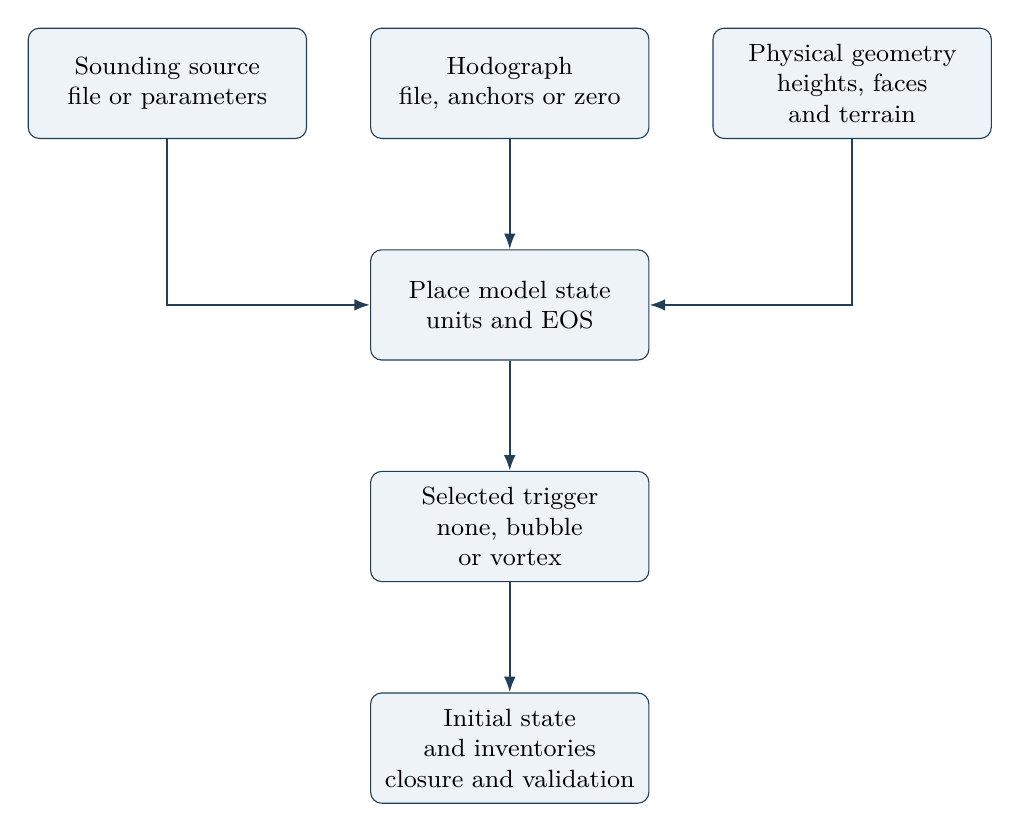
\begin{tikzpicture}[
 box/.style={draw=NimbusBlue,fill=NimbusLight,rounded corners,align=center,
             text width=3.3cm,minimum height=14mm,font=\small},
 flow/.style={-{Latex[length=2mm]},draw=NimbusBlue,thick},
 node distance=14mm and 8mm]
 \node[box] (column) {Sounding source\\file or parameters};
 \node[box,right=of column] (wind) {Hodograph\\file, anchors or zero};
 \node[box,right=of wind] (geometry) {Physical geometry\\heights, faces and terrain};
 \node[box,below=of wind] (placed) {Place model state\\units and EOS};
 \node[box,below=of placed] (trigger) {Selected trigger\\none, bubble\\or vortex};
 \node[box,below=of trigger] (initial) {Initial state\\and inventories\\closure and validation};
 \draw[flow] (column.south)|-(placed.west);
 \draw[flow] (wind)--(placed);
 \draw[flow] (geometry.south)|-(placed.east);
 \draw[flow] (placed)--(trigger);
 \draw[flow] (trigger)--(initial);
\end{tikzpicture}
\caption{Logical responsibilities in constructing an experiment. Environmental
thermodynamics, wind and geometry are separate inputs. A prescribed trigger
can change the initial water and energy inventories; it is not automatically
a conservative microphysical transfer. Exact execution and admission belong
to the initialization and configuration owners.}
\end{figure}


The \href{../include/init/sounding/sounding_source.hpp}{sounding contract},
\href{../include/init/hodograph/hodograph_source.hpp}{hodograph contract} and
\href{../include/init/trigger/trigger_source.hpp}{trigger contract} provide the
interfaces. \href{../src/init/scheme_profile.cpp}{Profile selection} and the
configuration compiler connect them to the ordinary runtime. A helper's
existence does not imply that every option it accepts is available through an
admitted public profile.

An initial environment also needs physical coordinate locations. A terrain
column may begin above the datum of an observed sounding, and its scalar and
velocity levels need not coincide. The initialized pressure, density and theta
must be interpreted through the production dry rho--theta relation. Moist
parcel diagnostics may use virtual temperature while the dynamical EOS uses a
dry pressure law; these are distinct approximations whose roles must be stated.

\section{Reading a sounding is a unit and representation conversion}

The public reader catalog offers \texttt{auto}, \texttt{cm1} and
\texttt{sharpy}. Automatic selection examines content and file signatures.
The reader family includes text and supported netCDF/HDF5 profile forms; a
filename extension alone does not identify a valid physical sounding.
The \href{../src/soundings}{sounding module} validates the supplied variables,
finite values, ordering, units, dimensions and model coverage before a profile
is used.

The mathematical input is a set of values at stated heights or pressure levels,
not a picture of a skew-T diagram. For example, a value written in grams of
vapor per kilogram of dry air must be divided by 1000 to become the solver's
kg/kg dry-air mixing ratio. A temperature in degrees Celsius must be converted
to kelvin before evaluating an exponential saturation formula. Confusing a
moist-air specific humidity $q_s=m_v/(m_d+m_v)$ with a dry-air mixing ratio
$r_v=m_v/m_d$ gives the wrong quantity even though both are dimensionless:
\[
 r_v=\frac{q_s}{1-q_s},\qquad q_s=\frac{r_v}{1+r_v}.
\]
A reader must know which definition the source supplies rather than infer it
from a small decimal value.

Strict-v1 file initialization retains automatic format routing, linear
interpolation, no extrapolation and no silent procedural fallback. The
lower-level fallback source remains compatibility code: its existence does
not authorize replacing a missing observation with an invented atmosphere
under the ordinary strict path. Sounding coverage of the required model heights
is therefore a real input requirement.

For a scalar quantity $a$ between valid source levels $z_j$ and $z_{j+1}$,
linear interpolation uses
\[
 a(z)=(1-\lambda)a_j+\lambda a_{j+1},\qquad
 \lambda=\frac{z-z_j}{z_{j+1}-z_j}.
\]
This preserves the endpoint values and is bounded between them for
$0\le\lambda\le1$. It is not a conservative remapping of a three-dimensional
mass inventory. That is acceptable only because it is being used to define a
new initial profile, with its resulting inventories diagnosed afterward.
Interpolating Cartesian wind components directly also avoids interpolating
across the discontinuity between directions near $0$ and $360$ degrees.

\section{Hydrostatic preparation and the model EOS must be distinguished}

For an idealized resting column, hydrostatic balance is
$dp/dz=-\rho g$. Combining an ideal-gas relation with a chosen temperature
profile gives an integral pressure relation, schematically
\[
 \log\frac{p(z_2)}{p(z_1)}
 =-\int_{z_1}^{z_2}\frac{g}{R_dT_v(z)}\,dz
\]
when the chosen preparation uses virtual temperature $T_v$. The dry version
uses $T$ instead. This equation states the assumptions used to build a profile;
it does not replace the solver's declared dry-density pressure law or prove
that a sampled profile is a discrete resting state.

Nimbus's parametric source constructs pressure along its idealized column and
diagnoses thermodynamic quantities from that construction. File input has its
own conversion and validation. Placement onto model fields, reference-state
construction and later EOS projection must remain consistent with their
respective definitions. A continuous hydrostatic relation and the discrete
pressure-gradient/gravity pairing are separate checks, as developed in the grid
chapter. A small initialization adjustment wave can reflect a mismatch between
them rather than an instability of the supplied atmosphere.

\section{CAPE targeting is a bounded inverse problem}

The \texttt{parametric\_cape} source builds an idealized mixed layer, a
free-tropospheric temperature lapse and a stable upper cap. Its moisture profile
uses the configured near-surface amount, a vertical decay and a relative-humidity
limit. The control variable used to fit CAPE is the free-tropospheric lapse rate,
not an arbitrary independent adjustment of every level.

A surface-parcel buoyancy diagnostic has the conceptual form
\[
 B(z)=g\frac{T_{v,p}(z)-T_{v,e}(z)}{T_{v,e}(z)},\qquad
 \mathrm{CAPE}=\int_{\rm LFC}^{\rm EL}\max(B,0)\,dz.
\]
The parcel and environment must use the same pressure and humidity conventions.
Nimbus's diagnostic estimates the lifting-condensation level, lifts the parcel
dry below it and with a retained moist lapse approximation above it, and
integrates resolved positive buoyancy. It also reports inhibition and the
associated characteristic heights. These quantities depend on the diagnostic
algorithm and vertical resolution, not just the name of the sounding.

The source bisects a lapse-rate interval from 0.0055 to
$0.0098\,\mathrm{K\,m^{-1}}$, seeking agreement within
$50\,\mathrm{J\,kg^{-1}}$, with at most 60 iterations. These are the current
implementation's search bounds and stopping rule. The final profile is still
returned after the iteration limit; the source alone is not a proof that every
requested target is realizable within that family. Requested and realized
CAPE must be distinguished and the applicable diagnostics/admission checked.
See \href{../src/init/sounding/sources/parametric_cape.cpp}{the CAPE source}
and \href{../src/init/sounding/diagnostics.cpp}{parcel diagnostics}.

The \texttt{parametric\_targets} branch translates a requested diagnostic set
into parameters for that same family. Surface moisture may be inferred from an
LCL target; a mixed-layer cap provides an inhibition control; requested LFC/EL
values influence the mixed-layer and upper-profile construction. Those controls
are coupled. CAPE, CIN, LCL, LFC and EL cannot generally be prescribed as five
independent exact numbers by this limited profile family. The
\href{../src/init/sounding/sources/parametric_targets.cpp}{target translator}
contains heuristics and explicit input bounds; the resulting diagnostics remain
the report of what was actually constructed.

\href{https://journals.ametsoc.org/abstract/journals/mwre/110/6/1520-0493_1982_110_0504_tdonsc_2_0_co_2.xml}{Weisman
and Klemp (1982)} supplies important context for studying buoyancy and shear in
idealized convective environments. A preset inspired by that literature is not
a claim that Nimbus reproduces the paper's entire environmental construction,
numerical model or storm evolution.

\section{Wind profiles and hodograph precedence}

A hodograph is the path traced by $(u(z),v(z))$ with height. Its differences
control vertical shear; its curvature affects storm-relative flow and rotation
diagnostics. Translating every wind vector by a constant changes storm-relative
interpretation unless the storm-motion reference is translated consistently.
It does not change the environmental vector shear between two levels.

Nimbus's \texttt{auto} hodograph policy uses sounding winds when they are
available. Otherwise it constructs the configured parametric profile.
\texttt{wk\_param} explicitly selects the parameterized wind, and
\texttt{zero} supplies a calm column. A file containing valid winds and an
explicit separate hodograph are therefore different experiments from the
automatic file-wind path.

The retained \texttt{wk\_param} implementation is piecewise linear in each
Cartesian component through anchors at the surface, 1 km and 6 km. Above 6 km
it holds the final wind constant. Between anchors $a,b$ it uses
\[
 (u,v)(z)=(1-\lambda)(u,v)_a+\lambda(u,v)_b,
 \qquad\lambda=\frac{z-z_a}{z_b-z_a}.
\]
The selector name is not a promise of an arbitrary smooth quarter-circle or a
complete reproduction of a published hodograph. The
\href{../src/init/hodograph/sources/wk_param.cpp}{implemented interpolation}
and \href{../src/init/hodograph/factory.cpp}{wind precedence} are explicit.
Sampling the environmental wind at the chosen scalar/face positions belongs to
initialization; it must not silently change the staggering contract used by
later transport.

\section{The warm bubble changes both heat and, conditionally, water}

The current Cartesian bubble helper uses distance $r$ from its specified
physical center and a compactly applied Gaussian factor
\[
 f(r)=\begin{cases}
       \exp(-9r^2/R^2),&r\le R,\\
       0,&r>R,
      \end{cases}
 \qquad\Delta\theta=\Delta\theta_{\max}f(r).
\]
Thus $R/3$ is the Gaussian width in this convention, and the field is cut off
at $R$ rather than extending to infinity. The helper retains a minimum radius
of 100 m and uses physical terrain height where active metrics are present.
Public validation and exact-profile admission additionally govern which settings
can reach that helper.

When pressure and vapor fields have matching shape and the applied theta
increment is positive, the helper scales vapor to retain its local saturation
ratio at the held pressure:
\[
 q_v^{\rm new}=q_v^{\rm old}
       \frac{q_{vs}(T^{\rm new},p)}{q_{vs}(T^{\rm old},p)}.
\]
The ratio is applied only when the old saturation amount exceeds the retained
small-value threshold. The helper uses its local liquid-water saturation fit
and an Exner exponent of 0.2857 for this conversion. Those are its actual
approximations; one should not assume that it calls the selected microphysics
scheme's saturation routine or performs a closed moist adjustment.

Optional cloud seeding separately adds a configured cloud-water amount times
$f(r)$. It is not subtracted from vapor as a condensation transaction. The warm
bubble therefore changes the initial thermal state and can add vapor and cloud
water. These are prescribed initial-condition changes. Their resulting mass and
energy belong in the initial inventory, rather than being mislabeled as a
conservative source during the first timestep. They also do not guarantee that
every chosen environment will produce sustained convection.

See \href{../src/core/orchestration/dynamics/initial_conditions_cartesian.cpp}{the
Cartesian initializer}. A trigger named \texttt{none} makes no such disturbance;
choosing it does not remove environmental instability or subsequent stochastic
forcing selected elsewhere.

\section{The Rankine seed has a defined profile and an implementation gap}

The \texttt{vortex\_seed} helper adds an azimuthal velocity around a horizontal
center. With radius $r_m$ of maximum wind and signed peak speed $V_m$,
\[
 v_\vartheta(r)=\begin{cases}
 V_m r/r_m,&0<r\le r_m,\\
 V_m r_m/r,&r>r_m,
 \end{cases}
 \qquad
 \Delta u=-v_\vartheta\frac{y-y_c}{r},\quad
 \Delta v=v_\vartheta\frac{x-x_c}{r}.
\]
The axis receives no singular increment. The source adds this wind to the
existing environmental field and applies a hard upper-height cutoff at
\texttt{z\_top\_m}. It does not construct an accompanying balanced pressure
perturbation. Sampling a continuous rotational formula also does not, by itself,
prove zero discrete divergence or exact balance on the selected staggered grid.

The public configuration currently parses and serializes
\texttt{center\_z\_m}, but this helper does not use it to place the vortex
vertically. Its applied placement uses the horizontal center and the upper
cutoff described above. This is a known initialization implementation gap;
the parameter must not be interpreted as an implemented vertical translation.
Exact admitted profiles still have their own restrictions, so this description
is not blanket admission of every vortex configuration. The concrete owner is
\href{../src/init/trigger/sources/vortex_seed.cpp}{the vortex-seed implementation}.

\section{Terrain shapes are also initial scientific inputs}

The terrain catalog provides \texttt{none}, \texttt{bell} and \texttt{schar}.
The flat choice does not imply uniformly spaced vertical levels; the geometry
owner can still provide stretched physical coordinates. A two-dimensional bell
ridge uses
\[
 h(x)=\frac{h_0}{1+(x/a)^2},
\]
while the axisymmetric bell uses
$h(x,y)=h_0a^3/(a^2+x^2+y^2)^{3/2}$. The Sch\"ar profile is
\[
 h(x)=H\exp[-(x/a)^2]\cos^2(\pi x/\ell).
\]
Height and width parameters have physical length units, and the source supplies
the corresponding slopes. These shapes define geometric input, not a physical
land-surface evolution model.

The mapping must turn that topography and the vertical grid into positive
physical layer volumes and compatible face metrics. A wind tangent to a slope,
an environmental profile sampled at the actual height, a surface flux per true
area and a radiation shadow are all consequences of the same terrain geometry.
They must not each reconstruct a different terrain from nominal spacing.
See \href{../src/terrain/base/topography.cpp}{the shape functions} and the
\hyperref[grid-deep-dive]{detailed grid chapter}.

\section{What should be recorded about an initialized experiment}

Retain the source profile or parameter values, wind-selection precedence,
physical grid and terrain, trigger settings, stochastic seed/member identity,
requested diagnostics and realized diagnostics. Record the initial dry mass,
water and energy basis after all prescribed interventions and closures. The
same file profile interpreted on a different grid, with a different trigger or
a different moisture convention is a different experiment even when its name
is unchanged.

The initial-condition and sounding tests under
\href{../tests/init}{tests/init} exercise parsing, thermodynamic conversion,
coverage, selection and trigger independence. The first evolution step then
checks a different contract: it must advance that accepted state through the
selected numerical and physical owners. Restart is different again; it restores
a continuation state and should not rerun an initial bubble or invent a new
sounding in place of saved scheme-private history.


\chapter{Grid, resolved dynamics and the coupled
timestep}\label{grid-theory}

This chapter develops the grid and time-integration arguments behind the
\href{MATHEMATICS.pdf}{mathematics overview}. It describes the Cartesian
atmosphere implemented in Nimbus. Equations written for a uniform,
stationary grid are introduced as explanatory cases; the mapped
operators must additionally use their physical metrics. The
implementation supports several discrete paths, and an equation in this
chapter does not imply that every configuration or backend combination
is admitted.

\section{Start with an inventory, not an array
value}\label{start-with-an-inventory-not-an-array-value}

A water mixing ratio is an amount of water divided by dry-air mass. It
is not itself the conserved water amount in a cell. If cell \(c\) has
physical volume \(V_c\), its dry mass and the inventory of a scalar
\(\phi\) are

\[\begin{aligned}
M_c &= \rho_{d,c} V_c, \\
Q_c &= M_c\phi_c.
\end{aligned}\]

For water, \(\phi\) is a species mixing ratio. For a particle number
stored per kg dry air, \(Q_c\) is the particle count. A number stored
per cubic metre would instead have inventory \(V_c N_c\). These
distinctions explain why the private microphysics transport interface
declares units: applying an identical array update to different units
would solve different conservation equations.

Integrate dry-mass continuity over the cell and apply the divergence
theorem. Let \(F_f\) denote outward dry-mass flow through face \(f\), in
kg s\(^{-1}\), averaged over the interval. A stationary finite-volume
update is

\[\begin{aligned}
M_c^{n+1} &= M_c^n-\Delta t\sum_{f\in\partial c}F_f, \\
Q_c^{n+1} &= M_c^n\phi_c^n
             -\Delta t\sum_{f\in\partial c}F_f\phi_f
             +\Delta Q_{c,\mathrm{source}}, \\
\phi_c^{n+1} &= Q_c^{n+1}/M_c^{n+1}.
\end{aligned}\]

An internal face has one flow and opposite signs in its two neighboring
cells. Its contribution therefore cancels from the domain sum. At a
physical boundary it remains an exchange with the exterior. This
cancellation, and the use of the same flow in both equations, are the
useful conservation properties.

For example, set every \(\phi\) to a constant \(\phi_0\) and omit
sources. Consistent reconstruction returns \(\phi_f=\phi_0\), so the
second equation becomes \(Q_c^{n+1}=\phi_0 M_c^{n+1}\). A uniform mixing
ratio stays uniform even while density changes. If scalar transport
recomputes a different mass flow, that identity no longer holds. Nimbus
therefore retains beginning density and the continuity interval flux
used to recover transported scalars. The relevant contracts are
\href{../include/numerics/advection/cartesian_mass_flux.hpp}{mass flux},
\href{../src/numerics/advection/advection_cartesian.cpp}{Cartesian
advection} and
\href{../include/microphysics/prognostic_transport.hpp}{private scalar
units}.

Array bounds are not physical integration bounds. Arrays include storage
used for closure and halos, and boundary values can be finite and quite
plausible. Including them in a mass sum would nevertheless count extra
atmosphere. The
\href{../include/core/infra/physical_cell_domain.hpp}{physical cell
domain} defines the half-open scalar ranges that belong to the
atmosphere. Operators must then identify the faces bounding those cells,
rather than infer the physical domain from a loop over every allocated
element.

\begin{figure}[htbp]
\centering
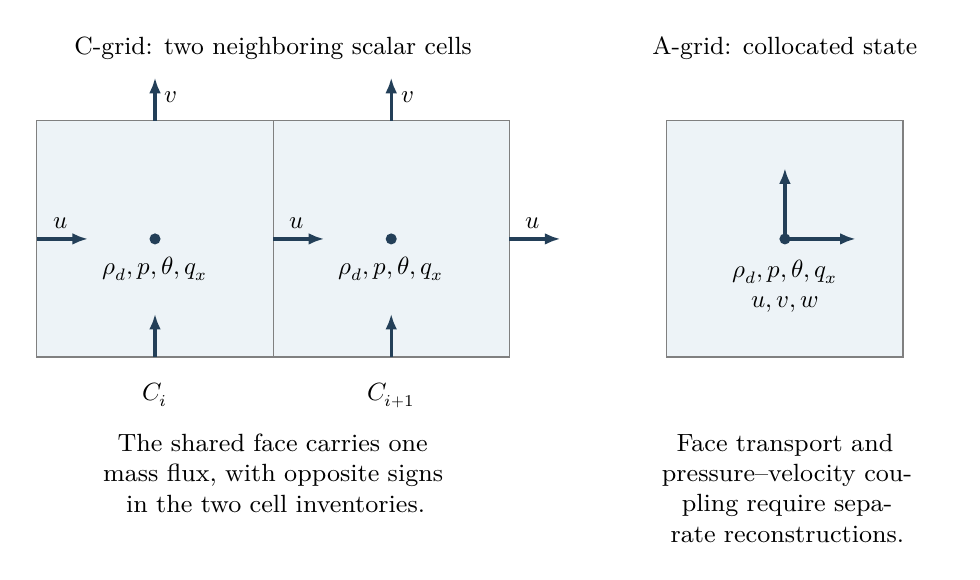
\begin{tikzpicture}[x=1cm,y=1cm,font=\small,
  velocity/.style={-{Latex[length=2mm]},very thick,draw=NimbusBlue}]
  \draw[fill=NimbusLight,draw=gray] (0,0) rectangle (6,3);
  \draw[draw=gray] (3,0)--(3,3);
  \node[above] at (3,3.65) {C-grid: two neighboring scalar cells};
  \foreach \x in {1.5,4.5} {
    \fill[NimbusBlue] (\x,1.5) circle (2pt);
    \node[below=3pt] at (\x,1.5) {$\rho_d,p,\theta,q_x$};
    \draw[velocity] (\x,0)--(\x,.55);
    \draw[velocity] (\x,3)--(\x,3.55);
    \node[right] at (\x,3.3) {$v$};
  }
  \foreach \x in {0,3,6} {
    \draw[velocity] (\x,1.5)--(\x+.65,1.5);
    \node[above] at (\x+.3,1.5) {$u$};
  }
  \node[below] at (1.5,-.2) {$C_i$};
  \node[below] at (4.5,-.2) {$C_{i+1}$};
  \node[anchor=north,align=center,text width=6cm] at (3,-.85)
    {The shared face carries one mass flux, with opposite signs in the two cell inventories.};
  \draw[fill=NimbusLight,draw=gray] (8,0) rectangle (11,3);
  \node[above] at (9.5,3.65) {A-grid: collocated state};
  \fill[NimbusBlue] (9.5,1.5) circle (2pt);
  \draw[velocity] (9.5,1.5)--(10.4,1.5);
  \draw[velocity] (9.5,1.5)--(9.5,2.4);
  \node[below=4pt,align=center] at (9.5,1.5) {$\rho_d,p,\theta,q_x$\\$u,v,w$};
  \node[anchor=north,align=center,text width=4cm] at (9.5,-.85)
    {Face transport and pressure--velocity coupling require separate reconstructions.};
\end{tikzpicture}
\caption{Horizontal plan views of the two layouts. On the C-grid, $w$ is stored
on the horizontal faces above and below each scalar volume and is omitted from
this plan view. The labels describe physical locations, not a universal array
index convention. Halo and closure locations are not additional atmospheric cells.}
\end{figure}


\section{Why the locations of pressure and velocity
matter}\label{why-the-locations-of-pressure-and-velocity-matter}

On the Cartesian C-grid, \(p\), \(\rho_d\), \(\theta\) and water
quantities are scalar cell values. Velocity components lie on their
respective normal faces. In the array convention, \(u(i,j,k)\) is the
east face of scalar cell \((i,j,k)\), \(v(i,j,k)\) is its north face,
and \(w(i,j,k)\) is its upper face. The lower ground face has a
separately owned boundary value. An index alone therefore does not
identify one common physical point for every field.

For two adjacent uniform-grid cells, the x-face dry-mass flow is
constructed from a density average and the already face-located wind:

\[F_{i+1/2}=A_{i+1/2}
\frac{\rho_{d,i}+\rho_{d,i+1}}{2}\,u_{i+1/2}.\]

Here \(A\) is physical face area. The mass-flux helper returns the
product before area integration. The pressure difference
\((p_{i+1}-p_i)/\Delta x\) is located at this same face, so the pressure
acceleration and normal velocity naturally share a location. Density
interpolation and the perturbation-pressure choice remain part of the
momentum operator; placement alone does not prove an energy identity.

The A-grid stores velocity at scalar locations. Its uncorrected face
product uses both interpolated density and interpolated velocity:

\[F^{\mathrm{raw}}_{i+1/2}
=A_{i+1/2}\frac{\rho_{d,i}+\rho_{d,i+1}}{2}
                    \frac{u_i+u_{i+1}}{2}.\]

That interpolation introduces a familiar pressure problem. Consider the
alternating pattern \(p_i=p_*+a(-1)^i\). Its centered cell gradient is
zero:

\[\frac{p_{i+1}-p_{i-1}}{2\Delta x}=0,
\qquad
\frac{p_{i+1}-p_i}{\Delta x}\ne 0\quad(a\ne0).\]

Thus a collocated cell-gradient operator can fail to see an oscillatory
pressure field that should drive face motion. Nimbus's
\texttt{CollocatedPressureCoupling} corrects the face velocity using the
direct pressure jump minus the interpolated cell pressure acceleration.
Continuity and retained scalar transport receive the same correction.
This coupling is deliberately inactive on the C-grid, whose face
velocity is already paired with an adjacent-cell pressure jump. The two
grids consequently have distinct numerical operators, not merely
different names for the same arrays.

Face placement also changes kinetic-energy accounting. Let \(M\) be a
scalar cell's moist-mixture mass and consider only its two x faces.
Assigning each face half the cell mass gives

\[\begin{aligned}
K_{x,\mathrm{faces}} &= \frac{M}{4}(u_L^2+u_R^2), \\
K_{x,\mathrm{center}} &= \frac{M}{2}
                         \left(\frac{u_L+u_R}{2}\right)^2, \\
K_{x,\mathrm{faces}}-K_{x,\mathrm{center}}
                    &= \frac{M}{8}(u_R-u_L)^2.
\end{aligned}\]

Averaging first and then squaring loses the positive contribution from
within-cell face variation. Summing the analogous x, y and z terms is
the scalar-cell representation of Nimbus's C-grid kinetic inventory. An
interior face gathers half-cell mass from each side; a physical boundary
contributes only its owned side. This is why an A-grid kinetic-energy
formula cannot be substituted into a C-grid diagnostic.

The mixture mass in this diagnostic is \(M=\rho_dV(1+q_t)\). It does not
change the density convention of the dynamical pressure acceleration.
The latter uses its declared dry-density approximation. The
\href{../src/dynamics/cartesian_cgrid_momentum_flux.cpp}{momentum-flux
owner} and
\href{../src/diagnostics/budgets/energy_budget.cpp}{energy-budget
implementation} must be assessed together when asking whether a
particular discrete force and transport preserve a chosen energy
inventory.

\section{What reconstruction adds to the flux
equation}\label{what-reconstruction-adds-to-the-flux-equation}

The finite-volume equations require a face scalar \(\phi_f\). A cell
average does not uniquely determine that value. First-order upwinding
uses the donor cell value; it is robust under an appropriate timestep
restriction but spreads sharp features. Higher-order reconstruction
estimates subcell variation. TVD limiting reduces a reconstructed slope
when neighboring data indicate an extremum or discontinuity. WENO5
combines candidate reconstructions with weights that respond to their
local smoothness, reducing the influence of a stencil that crosses a
sharp feature.

These are assumptions about what can be inferred between stored samples.
They do not add resolved information below the grid spacing. Their
formal order applies in sufficiently smooth regions, with compatible
boundaries and time integration. Limiters, positivity enforcement and
process thresholds can reduce local order. A narrow precipitation shaft
can therefore be sensitive to resolution even when its integrated mass
is well conserved.

Momentum has its own control volumes and transport paths. The
conservative C-grid momentum owner builds dual-volume fluxes from
dry-density transport. Other retained slow-tendency paths use
derivative-based advection. It would be incorrect to describe every
selectable path as one identical finite-volume discretization of the
complete moist Euler equations. The current configuration and
\href{../tests/numerics/test_advection_cartesian.cpp}{advection tests}
identify the actual operator being exercised.

\section{Pressure, gravity and the fast acoustic
response}\label{pressure-gravity-and-the-fast-acoustic-response}

Potential temperature provides a convenient adiabatic thermal variable.
With the retained constant dry-air parameters, Nimbus uses

\[\begin{aligned}
T &= \theta\left(\frac{p}{p_{\mathrm{ref}}}\right)^{\kappa_d},
&\kappa_d &= R_d/c_{pd}, \\
p &= p_{\mathrm{ref}}
       \left(\frac{\rho_dR_d\theta}{p_{\mathrm{ref}}}\right)^{\gamma_d},
&\gamma_d &= \frac{c_{pd}}{c_{pd}-R_d}.
\end{aligned}\]

These relations imply \(p=\rho_dR_dT\). Moisture is not inserted into
this pressure relation as an additional gas constant. That is a
deliberate retained model convention. Phase heating, vapor buoyancy,
condensate loading and the moist diagnostic energy are separate parts of
the implementation.

To see why this system supports fast waves, linearize about a uniform
resting dry state, holding \(\theta\) fixed during the acoustic
perturbation. Then \(p'=c_s^2\rho_d'\) with
\(c_s^2=\gamma_dp_0/\rho_{d0}\). Linear continuity and momentum give

\[\begin{aligned}
\partial_t\rho_d' + \rho_{d0}\nabla\!\cdot\boldsymbol u' &= 0, \\
\partial_t\boldsymbol u' &= -\rho_{d0}^{-1}\nabla p', \\
\partial_{tt}\rho_d' &= c_s^2\nabla^2\rho_d'.
\end{aligned}\]

The final equation is the acoustic wave equation for this simplified
limit. It explains why an advectively acceptable large step may still be
unstable for pressure waves. Nimbus's acoustic policy increases the
configured minimum number of substeps using current sound speed and
minimum physical spacing. The retained estimate uses a target acoustic
Courant number of 0.5 and an additional substep beyond the ceiling
estimate. This is an implementation stability policy, not proof of
accuracy for an arbitrary physical timestep.

In a stratified atmosphere, pressure and gravity are each large. A
reference column satisfies the intended background balance, and
perturbation operators resolve the departure from it. For the flat
C-grid vertical force, the retained terms have the form

\[\begin{aligned}
a_w ={}&-\frac{1}{\rho_d}\partial_z(p-p_0)
        -g\frac{\rho_d-\rho_{d0}}{\rho_d} \\
       &+0.608g(q_v-q_{v0})
        -g(q_c+q_r+q_i+q_s+q_g+q_h),
\end{aligned}\]

with quantities interpolated to their velocity location. The
perturbation pressure force belongs to the fast update; the other
displayed contributions belong to the slow preparation. The vapor term
approximates virtual-temperature buoyancy, while condensate contributes
loading. Adding a separate thermal buoyancy formula on top of the
existing perturbation-density term would change the model and can
double-count the thermal effect. See the
\href{../src/dynamics/schemes/klemp_wilhelmson_split/cartesian_cgrid_3d.cpp}{C-grid
tendency implementation} and
\href{../src/dynamics/schemes/klemp_wilhelmson_split/cartesian_common.hpp}{shared
Cartesian force helpers}.

\section{Terrain and moving coordinates change the
geometry}\label{terrain-and-moving-coordinates-change-the-geometry}

Let a terrain-following mapping be \(z=z(x,y,\zeta)\). Even though
arrays remain rectangular in index space, physical cells need not have
equal volumes or orthogonal faces. The coordinate Jacobian changes the
amount of atmosphere represented by a coordinate-space volume. Physical
gradients require metric terms, and the normal velocity through a mapped
face is generally a combination of Cartesian velocity components.

For a stationary lower boundary \(z=h(x,y)\), impermeability says that
the wind is tangent to the surface. Taking the material derivative of
\(z-h(x,y)=0\) gives

\[w=u\,\partial_xh+v\,\partial_yh.\]

Thus zero normal flow can coexist with nonzero physical vertical
velocity. Energy basis v2 includes the diagnosed ground-face kinetic
contribution, rather than treating this face as implicitly motionless.
On stretched layers, scalar center distances, layer thicknesses and
velocity dual-volume widths must also be distinguished. A single nominal
\(\Delta z\) is not an adequate substitute.

A moving control volume changes the transport velocity. Reynolds
transport gives the relevant normal flux as

\[F_f=\rho_{d,f}
     (\boldsymbol u_f-\boldsymbol v_{g,f})\!\cdot\boldsymbol n_f\,A_f,\]

where \(\boldsymbol v_g\) is grid velocity. Nimbus retains Earth-frame
wind and subtracts grid translation when constructing the relative flux.
Adding grid velocity to every stored wind during a window shift would
change the physical state. Earth-fixed terrain and terrain attached to a
translating computational frame also pose different boundary problems.

Window movement and nesting require conservative remapping of
inventories, consistent velocity locations, and ownership of
boundary/feedback exchanges. Interpolating only visible water and wind
fields would leave private particle moments, held physical sources and
restart state inconsistent. The
\href{../include/terrain/conservative_transport.hpp}{terrain transport
interface},
\href{../tests/dynamics/test_mapped_reconstruction.cpp}{mapped
reconstruction tests},
\href{../tests/dynamics/test_native_moving_energy.cpp}{moving-energy
tests} and \hyperref[grid-deep-dive]{the detailed grid chapter} describe these additional
contracts.

\section{How the split timestep is
assembled}\label{how-the-split-timestep-is-assembled}

\href{https://journals.ametsoc.org/abstract/journals/atsc/35/6/1520-0469_1978_035_1070_tsotdc_2_0_co_2.xml}{Klemp
and Wilhelmson (1978)} provide the physical and numerical motivation for
separating compressible acoustic motion from slower cloud-scale
evolution. Nimbus implements a specific callback sequence rather than
reproducing an entire published model unchanged. The following describes
its split-explicit path; SSPRK3 and RK4 have separate stage owners.

At the outer runtime level, radiation and boundary-layer sources are
refreshed when their cadence requires it. Held sources remain physical
state with an interval of validity. The dynamics owner prepares slow
tendencies, including applicable advection, forcing and buoyancy. Where
the configured slow-stage method requires a predictor, it constructs the
corresponding tendency average and restores the authoritative stage
state before the final advance.

The split integrator first applies the slow increment over the large
timestep. It seeds radiative acoustic boundary history from that
post-slow state. Each acoustic substep then advances pressure/density,
closes the pressure/density boundaries needed by the next operation, and
advances momentum using the newly available pressure and density.
Boundary time advancement has its own owner; a final zero-duration
closure must not advance a radiative boundary a second time. Native
batched implementations must preserve this sequencing even when their
implementation does not make one host call per substep.

The production CPU pressure commit updates dry density through
continuity, stores the new float density and diagnoses pressure through
the dry rho--theta EOS from the stored density and potential
temperature. A pressure tendency buffer alone is therefore not the
complete description of the committed pressure state. This distinction
matters when evaluating pressure work and storage-rounding
contributions.

After the acoustic sequence, the runtime recovers thermodynamic and
tracer transport using the retained continuity flux when the selected
path has not already coupled that transport. It also transports declared
private microphysics state. Microphysics then produces and commits its
source changes. Applicable explicit SGS and diffusion follow, and a
final pressure projection restores the algebraic rho--theta EOS
relation. Sponge and final boundary operations have their subsequent
ownership. The exact conditionals belong to
\href{../src/core/orchestration/dynamics/dynamics.cpp}{dynamics
orchestration}, the
\href{../src/numerics/time_stepping/schemes/split_explicit/split_explicit.cpp}{split
integrator} and \href{../src/core/runtime/headless_runtime.cpp}{headless
runtime}.

This order has a scientific consequence: a private microphysics cell
helper that assumes its source is followed immediately by EOS projection
cannot be inserted into the live solver without accounting for
intervening SGS/diffusion and other state changes. The guarded
source/EOS transaction is tested as an explicit endpoint mapping; its
complete field-level runtime integration remains Engineering incomplete.

For comparison, an autonomous SSPRK3 system \(y_t=L(y)\) has the
standard convex stage structure

\[\begin{aligned}
y^{(1)} &= y^n+\Delta tL(y^n), \\
y^{(2)} &= \tfrac34y^n+\tfrac14[y^{(1)}+\Delta tL(y^{(1)})], \\
y^{n+1} &= \tfrac13y^n+\tfrac23[y^{(2)}+\Delta tL(y^{(2)})].
\end{aligned}\]

The corresponding final tendency weights are \(1/6\), \(1/6\) and
\(2/3\). Classical RK4 uses four tendency weights \(1/6\), \(1/3\),
\(1/3\) and \(1/6\). These formal orders assume a consistently evaluated
right-hand side. Cadence holding, phase switches and limiter activation
can change the accuracy of the coupled model. Nimbus must stage and
restore primary fields, private moments and reports consistently if any
stage fails. The
\href{../tests/numerics/test_time_stepping.cpp}{time-integration tests}
and \href{../tests/numerics/test_runtime_timestep.cpp}{runtime timestep
tests} check different parts of this requirement.

\section{A concrete mass--heat--pressure
example}\label{a-concrete-massheatpressure-example}

Consider an illustrative scalar cell containing 10 kg of dry air and a
uniform vapor mixing ratio of 0.01. During transport, 2 kg of dry air
enters and 1 kg leaves, carrying the same mixing ratio. Its final dry
mass is 11 kg; vapor mass is \(0.1+0.02-0.01=0.11\) kg, so its mixing
ratio remains 0.01. Using the old 10 kg denominator after updating vapor
mass would incorrectly produce 0.011. This elementary example is the
reason continuity and scalar transport share one flux history.

Next suppose a liquid-phase source condenses \(2\times10^{-4}\) kg per
kg dry air. The source removes that amount from vapor and adds it to
cloud liquid, so total water is unchanged. Under the ordinary
constant-\(c_{pd}\) latent-heating convention, its temperature increment
is

\[\Delta T_{\mathrm{source}}
=\frac{L_v}{c_{pd}}\,2\times10^{-4}\simeq0.498\ \mathrm{K}.\]

At held stage pressure, this becomes
\(\Delta\theta=\Delta T_{\mathrm{source}}/\Pi\) with
\(\Pi=(p/p_{\mathrm{ref}})^{\kappa_d}\). This example illustrates the
units and the phase-source convention; a real saturation solver
determines the amount from the coupled saturation/heating calculation
rather than accepting an arbitrary condensation amount.

Now isolate the later dry-EOS projection and suppose the initial cell
was EOS-consistent, with \(T=280\) K. Hold its post-transport dry
density fixed and omit all intervening sources for this illustration. In
exact arithmetic the new EOS temperature is

\[T_{\mathrm{EOS}}=T
\left(1+\frac{\Delta T_{\mathrm{source}}}{T}\right)^{\gamma_d}.\]

To first order its increase is \(\gamma_d\Delta T_{\mathrm{source}}\),
about 0.70 K, rather than 0.498 K. The difference follows from the
retained thermal source convention and the subsequent pressure
diagnosis; it cannot be removed from the explanation by silently
replacing \(c_p\) with \(c_v\). Actual float storage adds a further
small contribution. In the full runtime, intervening operators also
contribute and require their own attribution.

Nimbus's energy accounting records committed source and EOS changes. A
closed ledger says those changes have been assigned consistently.
Establishing that the complete thermal/mechanical exchange is physically
conservative requires the stronger coupled source, EOS, transport and
boundary argument. The
\href{../tests/diagnostics/test_energy_budget.cpp}{energy tests} and
guarded
\href{../tests/physics/test_milbrandt_triple_source_eos_energy.cpp}{source/EOS
tests} make that distinction explicit.

\section{Boundaries complete the
equations}\label{boundaries-complete-the-equations}

A periodic domain cancels opposing boundary exchanges. A closed physical
wall imposes its normal-flow constraint and may still have thermal or
tangential stress fluxes if the chosen surface model supplies them. An
open boundary lets mass, momentum and energy leave or enter. Radiative
conditions approximate outgoing disturbances using a finite history;
they are neither exact exterior solutions nor permission to reuse stale
stage data.

Sponge and Rayleigh terms deliberately relax fields. They can remove or
add kinetic and thermal energy according to the target state.
Sedimentation removes water through the lower surface, while radiation
transports energy through the top and bottom of a column. Consequently a
domain energy curve is meaningful only alongside those exchange terms
and the chosen inventory basis. The
\href{../tests/dynamics/test_cartesian_boundary_conditions.cpp}{boundary
tests} and
\href{../tests/dynamics/test_native_cgrid_boundary.cpp}{native C-grid
boundary tests} exercise these conditions at their actual locations and
stages.

Neither a stable integration nor an accounting identity is a complete
validation of a storm simulation. Resolution sensitivity, physical
source references, supported coupling, restart, backend parity and
scientific review remain separate questions. The runtime catalog and
repository readiness contract determine which combination can make which
claim.

\chapter{The grid as a physical and numerical model}\label{grid-deep-dive}

A grid does more than select where an equation is evaluated. It decides which
volume owns mass, which surface carries a flux, which neighboring states can
influence one another, and which motions can be represented. These decisions
must agree between dynamics, microphysics, terrain, diagnostics and output.
This chapter develops those agreements from simple cases before considering
stretched grids and nested domains. The derivations below explain constraints
on the implementation; they are not claims that every Nimbus operator is an
exact realization of every identity derived here.

\section{A cell average, a sample and an inventory are different objects}

Let $C$ be a physical cell with volume $V_C$. For a continuous density field,
the cell-average dry density is
\[
 \overline{\rho_d}_C=\frac{1}{V_C}\int_C\rho_d\,dV,
 \qquad M_C=V_C\overline{\rho_d}_C.
\]
If a vapor field varies inside the cell, the dry-mass-weighted mixing ratio is
\[
 \widetilde q_{v,C}
 =\frac{\int_C\rho_d q_v\,dV}{\int_C\rho_d\,dV},
 \qquad W_{v,C}=M_C\widetilde q_{v,C}.
\]
In general, this weighted average is not the arithmetic volume average of
$q_v$, and neither average has to equal the value at the geometric center.
Writing one floating-point number per cell necessarily chooses a representation
of the unresolved variation. Nimbus's conservative scalar transport treats
$\rho_d V$ as the carrier inventory and $Mq$ as the transported species
inventory. A plotted center value is a reconstruction of that representation.

The distinction matters even in an apparently simple two-cell average. Suppose
two equal-volume cells contain dry masses of 2 and 1 kg and have mixing ratios
of 0.01 and 0.02. Their total water is 0.04 kg and total dry mass is 3 kg, so the
combined mixing ratio is $0.04/3$. The arithmetic mean, 0.015, would imply
0.045 kg of water after combining them. No equation of state or more accurate
color map can repair that inventory error afterward. Restriction, remapping
and budget calculations must preserve the mass weights at the operation that
changes the representation.

Nimbus is not uniformly a finite-volume discretization of every prognostic
quantity. Scalar continuity and conservative transport have explicit inventory
contracts; velocity tendencies, pressure projection and closures have their own
discrete forms. The conservation of one scalar update does not establish a
conservative total-energy discretization of the complete model. The useful
question is which identity an operator satisfies, using which state and which
geometry, rather than whether the entire program is given one numerical label.

\section{Allocated dimensions are not the atmospheric domain}

The arrays are contiguous containers with index
\[
 \ell(i,j,k)=(iN_y+j)N_z+k.
\]
The last index is contiguous in memory. This is a storage rule, not a definition
of a cell's physical volume or a promise that each index is an independent
atmospheric cell. The historical member names \texttt{nr} and \texttt{nth}
are also used by Cartesian paths; their spelling does not make those paths
cylindrical. Coordinates, staggering and the declared physical domain supply
the interpretation.

\href{../include/core/infra/physical_cell_domain.hpp}{PhysicalCellDomain}
uses half-open ranges, so $i_{\rm begin}\le i<i_{\rm end}$ owns scalar
control volumes. In the ordinary arrays with at least three points on an axis,
one horizontal plane at each side is boundary-closure storage. The collocated
layout similarly excludes one plane at each vertical end when there are at
least three vertical entries. The C-grid scalar layout retains its vertical
scalar layers, with its ground-face velocity handled separately. Tiny arrays
used by bounded tests have explicit special cases; do not derive a universal
halo width from a single fixture.

For example, an allocated $10\times8\times6$ scalar array has 480 storage
locations. Under the C-grid ownership rule it contains $8\times6\times6=288$
physical scalar cells. Under the ordinary collocated rule it contains
$8\times6\times4=192$. These counts describe the current ownership helper,
not recommended simulation dimensions. Multiplying 480 by a nominal cell
volume would count closure state as additional atmosphere in either example.
Likewise, inferring the physical domain length from the allocation alone can
change a prescribed wavelength, mean density or column depth.

A halo can contain a finite, plausible value copied from an interior cell.
That does not give it volume. It exists so a stencil can read a defined neighbor,
so a boundary algorithm can retain history, or so a restart can reproduce the
same closure state. A valid restart may therefore retain more data than a
physical inventory integrates. Output metadata must carry the ownership range
rather than asking a reader to guess it from zeros, NaNs or array dimensions.

\section{Three distances that must not be collapsed into one}

Consider a flat but vertically stretched column. Let the lower and upper
interfaces of layer $k$ be $z_{k-1/2}$ and $z_{k+1/2}$, and let its representative
scalar height be $z_k$. The layer thickness is
\[
 h_k=z_{k+1/2}-z_{k-1/2},
\]
whereas the distance used by a center-to-center pressure gradient is
$d_{k+1/2}=z_{k+1}-z_k$. A vertical-velocity dual control volume spanning two
adjacent scalar centers has a width related to $d_{k+1/2}$, not automatically
to either neighboring $h_k$. All three distances coincide in a special uniform
construction; that coincidence is the reason the distinction can disappear
unnoticed in a uniform-grid implementation.

For a piecewise linear reconstruction between two scalar locations, the value
at an intermediate interface $z_f$ is
\[
 \phi_f=\frac{z_{k+1}-z_f}{z_{k+1}-z_k}\phi_k
       +\frac{z_f-z_k}{z_{k+1}-z_k}\phi_{k+1}.
\]
A simple half-sum is justified only when the face is halfway between those
locations. An independently reconstructed upwind value is a different numerical
choice. Neither should be substituted for the other just because both functions
return a value at an interface.

The divergence of a vertical flux density $f$ in layer $k$ is
$(f_{k+1/2}-f_{k-1/2})/h_k$. The gradient at an interior interface instead uses
$(\phi_{k+1}-\phi_k)/d_{k+1/2}$. Substituting one global $\Delta z$ into both
expressions changes the amount of transport per layer and the force between
layers. It can also destroy the cancellation between a base pressure gradient
and gravity while leaving the fields visually smooth.

The \href{../include/core/infra/physical_grid_metrics.hpp}{physical metric
interface} validates scalar centers, interfaces and positive layer thicknesses
and supplies the geometry used by column physics. It rejects a partly initialized
flat geometry and a terrain geometry whose shape does not match the fields.
Radiation, sedimentation, vertical mixing and diagnostics must consume that
same physical column. A radiation heating rate based on a nominal layer depth
while transport uses the actual depth is a coupling inconsistency, not merely
a small plotting discrepancy.

\section{Why C-grid staggering changes resolved waves}

The C-grid locates a normal velocity at the face through which it transports
mass. In Nimbus's index convention, $u(i,j,k)$ is the east face of scalar cell
$(i,j,k)$, $v(i,j,k)$ its north face and $w(i,j,k)$ its upper face. Thus the west
face used by a cell is addressed with the neighboring index. The separately
owned lower ground face is an important endpoint of the vertical construction.
A physical scalar interval of $n$ cells has $n+1$ boundary-and-interior face
locations in a nonperiodic direction. Under periodic conditions the end faces
represent one physical connection and must not become two distinct exchanges
in an inventory sum.

The benefit can be seen without a storm simulation. For a uniform one-dimensional
pressure perturbation $p_j=\widehat p\exp(\mathrm{i}kj\Delta x)$, a collocated
centered gradient has the Fourier factor
\[
 \frac{p_{j+1}-p_{j-1}}{2\Delta x}
 =\mathrm{i}\frac{\sin(k\Delta x)}{\Delta x}p_j.
\]
It is blind to the alternating grid-scale pattern at $k\Delta x=\pi$. A
center-to-face C-grid difference instead has magnitude
$2\sin(k\Delta x/2)/\Delta x$ after accounting for the half-cell phase shift.
It does not vanish at that wavelength. This explains one pressure--velocity
coupling advantage of staggering. It does not imply that a two-cell wave is
accurate or that an A-grid implementation cannot provide a different consistent
coupling with its own stabilization and reconstruction.

For the illustrative linear acoustic pair
$p_t=-\rho_0c^2 D u$ and $u_t=-G p/\rho_0$, a compatible C-grid divergence
and gradient on a periodic uniform grid give
\[
 \omega_h^2=c^2\left[\frac{2\sin(k\Delta x/2)}{\Delta x}\right]^2.
\]
The continuous relation is $\omega^2=c^2k^2$. Their difference is a spatial
dispersion error before the time integrator contributes any additional error.
At small $k\Delta x$, expanding the sine shows convergence to the continuous
wave; near the shortest represented wavelength, the discrete phase and group
velocities differ substantially. Increasing the formal order of an unrelated
microphysics source does not repair that wave dispersion.

A nominal grid spacing therefore does not equal the smallest accurately
resolved physical structure. The useful resolved range depends on the complete
spatial operator, filtering, time step, closures and the diagnostic being
measured. A resolution study must compare that diagnostic across grids under
consistent physical assumptions. Holding a number of grid cells fixed while
changing $\Delta x$ changes the physical size of a perturbation; holding a
Smagorinsky coefficient fixed while changing its grid-derived filter width
changes the modeled subgrid diffusivity.

\section{Flux cancellation is a topology statement}

Assign each interior face one orientation and one numerical dry-mass flow $F_f$.
Let $B_{Cf}$ be $+1$ when that orientation points outward from cell $C$, $-1$
when it points inward, and zero otherwise. The update is
\[
 M_C^{n+1}=M_C^n-\Delta t\sum_f B_{Cf}F_f.
\]
An interior column of $B$ contains one $+1$ and one $-1$. Summing over all
physical cells cancels that face exactly in real arithmetic, regardless of
whether the reconstruction is first or fifth order. What remains is the
physical boundary flux. This is the fundamental topological reason shared
fluxes conserve an inventory.

If the two adjacent cells separately reconstruct and round what is supposed to
be the same interface flow, they can use $F_f+\epsilon_L$ and
$F_f+\epsilon_R$. The domain acquires a residual proportional to
$\epsilon_L-\epsilon_R$. Thread safety alone does not establish a shared flux:
two race-free calculations can still disagree. Conversely, deterministic
summing of a wrong set of volumes does not make an inventory physical.

For a mixing ratio, Nimbus's retained continuity flux provides the same carrier
flow to the species update,
\[
 Q_C^{n+1}=Q_C^n-\Delta t\sum_f B_{Cf}F_f q_f,
 \qquad q_C^{n+1}=Q_C^{n+1}/M_C^{n+1}.
\]
When $q_f=q_0$ everywhere, the uniform value survives exactly in real arithmetic:
$Q_C^{n+1}=q_0 M_C^{n+1}$. This is stronger than obtaining the correct domain
sum alone. A scheme can preserve total water yet generate false cell-scale
concentration changes if it transports a different dry-mass carrier. The
retained-flux transport contracts test this consistency along with positivity
and invalid-input behavior.

The algebra also exposes a time-level requirement. If $Q_C^n$ is constructed
from an already updated density and an old mixing ratio, it is not the old
inventory. Saving the old carrier, or constructing the inventory before the
carrier is overwritten, is part of the mathematical scheme. Eliminating that
snapshot for performance requires an equivalent ownership arrangement. It is
not safe merely because no API signature changes.

\section{Reconstruction determines accuracy; limiting determines admissibility}

A face flow needs a transported value. In a positive one-dimensional flow, a
first-order upwind method takes the value from the cell on the inflow side.
For constant velocity $a>0$ and uniform spacing, the update is
\[
 q_j^{n+1}=(1-C)q_j^n+Cq_{j-1}^n,
 \qquad C=a\Delta t/\Delta x.
\]
For $0\le C\le1$, the new value is a convex combination and cannot exceed the
two contributing extrema. This explanatory result assumes a constant carrier,
no source and the stated first-order discretization. It is not a universal
positivity proof for a compressible, multidimensional, source-coupled update.

A linear reconstruction uses a slope to represent subcell variation and
reconstruct left and right interface states. An unlimited centered slope is
accurate on a smooth field but may produce negative condensate next to a sharp
edge. A limiter reduces the slope when the neighboring differences suggest an
extremum or discontinuity. WENO methods instead combine candidate
reconstructions with smoothness-dependent weights. Their motivation is to
recover high order in smooth regions while avoiding an oscillatory stencil
near a sharp feature. The reconstruction, its limiting, its boundary stencil
and its time integration must be evaluated together.

Nimbus's \href{../src/numerics}{numerical implementations} and the retained
\href{../tests/numerics}{numerical tests} define the admitted transport paths.
The method name does not establish high-order convergence everywhere: a limiter
can intentionally revert toward lower order, a boundary may use a shorter
stencil, and a phase source can introduce nonsmooth behavior. A resolution
comparison should report where the observed error comes from, rather than
assigning the formal smooth-field order to an entire convective storm.

Clipping a negative mixing ratio after a flux update changes its inventory.
If a stored cell would contain $Mq=-\delta$ and is simply set to zero, the
operation adds $\delta$ to the domain water amount. Small clipping is therefore
not automatically harmless. A conservative correction must identify where the
corresponding amount is removed, respect the available donor inventory, and
report the adjustment. A physical source limiter has a related duty: multiple
processes cannot each consume the same full reservoir independently.

\section{Pressure work needs compatible scalar and velocity geometry}

On a uniform grid with periodic boundaries, summation by parts gives a discrete
counterpart of the continuous pressure-work identity. For an interior face
between left and right cells with area $A_f$ and center distance $d_f$,
\[
 \sum_C V_C p_C(Du)_C
 =\sum_f A_f u_f(p_L-p_R)
 =-\sum_f A_f d_f u_f(Gp)_f.
\]
The velocity dual volume is $V_f^*=A_fd_f$. At a physical boundary there is an
additional boundary pressure-work term. This identity depends on using the same
face orientation, areas and center distances on both sides. Interpolating a
pressure gradient with one geometry and diagnosing work with another breaks
the pairing.

If the velocity equation uses $\rho_f\,du_f/dt=-(Gp)_f$, multiplying by
$V_f^*u_f$ supplies the kinetic-energy pressure work. Its partner in the internal
energy equation has the opposite sign. This is a design criterion for a coupled
energy discretization. Nimbus's diagnosed energy budgets and pressure/EOS
operators must be assessed against their actual discrete contracts; the
continuous identity by itself does not prove exact total-energy conservation
for the implemented rho--theta model.

A staggered kinetic inventory must first decide which cell mass weights its
velocity locations. As an illustrative dry inventory, retain the dry mass $M_C$
defined above. On a flat grid, assigning half of each adjacent cell's mass gives
\[
 M_f^*=\tfrac12M_L+\tfrac12M_R,
 \qquad K_f=\tfrac12M_f^*u_f^2.
\]
Boundary faces, vertical stretching and mapped ground motion require the
appropriate half-volume and metric construction. Averaging velocity to scalar
centers and then squaring is a different functional because the square of an
average is not the average of squares. Nimbus's moist-mixture basis-v2 diagnostic
instead uses cell masses $M_C^{\rm mix}=\rho_{d,C}V_C(1+q_{t,C})$ in this
half-cell construction. That diagnostic choice does not change the dynamical
pressure-force convention, which uses its declared dry-density approximation.
The flat-grid
\href{../src/diagnostics/budgets/velocity_energy_pair.cpp}{velocity/energy
pairing implementation} and the full
\href{../src/diagnostics/budgets/energy_budget.cpp}{energy diagnostic} make the
mass basis and geometric scope explicit.

Time discretization adds another issue. At fixed face mass, an impulse $I$
changes velocity by $I/M_f^*$ and changes kinetic energy by
\[
 \Delta K_f=u_f^n I+\frac{I^2}{2M_f^*}.
\]
The second term is missing if work is calculated using only the old velocity.
When face mass also changes, a term for that mass change is required. For
example, the exact endpoint decomposition
\[
 \Delta K_f=\tfrac12 M_f^{*,n+1}
  \big[(u_f^{n+1})^2-(u_f^n)^2\big]
 +\tfrac12\big(M_f^{*,n+1}-M_f^{*,n}\big)(u_f^n)^2
\]
is algebraically valid but assigns work differently from a midpoint-based
construction. An energy report must declare its endpoint basis; combining
terms from two different decompositions can double-count a contribution.

\section{Terrain is a coordinate transformation, not a tilted picture}

For the explanatory mapping $(x,y,\zeta)\mapsto(x,y,z(x,y,\zeta))$, define
$J=z_\zeta>0$, $z_x=(\partial z/\partial x)_\zeta$ and
$z_y=(\partial z/\partial y)_\zeta$. Chain rules give
\[
 \begin{aligned}
 (\partial_x\phi)_z&=(\partial_x\phi)_\zeta
                         -\frac{z_x}{J}\partial_\zeta\phi,\\
 (\partial_y\phi)_z&=(\partial_y\phi)_\zeta
                         -\frac{z_y}{J}\partial_\zeta\phi,\\
 \partial_z\phi&=\frac{1}{J}\partial_\zeta\phi.
 \end{aligned}
\]
Nimbus's mapped transport interface uses $G_x=-z_x$ and $G_y=-z_y$ with this
Jacobian convention. The signs are part of the interface. Reusing a formula
from a paper whose metric symbols have the opposite sign without converting
it can reverse the terrain correction while preserving dimensions.

For a stationary mapping the contravariant vertical coordinate velocity is
\[
 \dot\zeta=\frac{w-u z_x-v z_y}{J}.
\]
The transformed dry-mass equation can be written
\[
 \partial_t(J\rho_d)+\partial_x(J\rho_d u)
 +\partial_y(J\rho_d v)
 +\partial_\zeta\{\rho_d(w-u z_x-v z_y)\}=0.
\]
This equation is written for the stated mapping and continuous metrics. A
finite-volume implementation must still construct compatible discrete face
metrics, fluxes and physical volumes. It cannot obtain that compatibility merely
by evaluating the continuous expressions independently at arbitrary points.

At stationary terrain $z=h(x,y)$, zero normal flow requires
$w=u h_x+v h_y$. Setting the Cartesian vertical velocity to zero instead imposes
a different condition unless the terrain is locally flat or the wind has no
component along the slope gradient. A column's lower interface can therefore
have a physical vertical-velocity contribution even when no mass crosses the
ground. The distinction carries into surface stress, terrain pressure work and
the staggered kinetic inventory.

A useful geometric consistency check is free-stream preservation. A constant
physical velocity field should not acquire spurious divergence solely because
coordinate surfaces slope. The discrete metric construction must allow the
corresponding face contributions to cancel. A second check is hydrostatic
balance: pressure and gravity should cancel for the declared resting base
state using the same physical heights and averaging. These are different tests.
Passing one does not prove the other or establish the accuracy of transport
through a sharp terrain transition.

See the \href{../include/terrain/conservative_transport.hpp}{mapped gradient
and transport contract},
\href{../src/terrain/base/conservative_transport.cpp}{its implementation}, and
\href{../tests/dynamics/test_mapped_reconstruction.cpp}{mapped reconstruction
checks}. The \href{https://www2.mmm.ucar.edu/wrf/site/documentation/technote.html}{WRF
technical notes} provide a useful comparison with a mature terrain-following
solver. WRF's vertical coordinate and complete equation set are not Nimbus's;
that reference motivates questions about metrics and staggering rather than
supplying an interchangeable formula set.

\section{A moving window is not a new physical wind}

For a moving physical control volume, Reynolds transport uses relative normal
velocity $(\boldsymbol u-\boldsymbol v_g)\cdot\boldsymbol n$. If the window
translates horizontally with velocity $\boldsymbol U_g$, a stationary Earth-frame
parcel flows backward through that window even though its physical wind is
zero. Stored Earth-frame momentum must not be incremented by a window shift.
The relative transport velocity and the physical velocity used for kinetic
energy have different purposes.

A continuously deforming coordinate system also obeys the geometric conservation
law: the change in its volume must match the surface integral of grid velocity.
That is a constraint on a general moving-grid discretization, not a claim that
Nimbus implements unrestricted mesh deformation. Nimbus's domain controls,
integer relocation, terrain placement and supported nesting profiles have
specific execution and admission contracts. A discrete relocation is a remap
operation with retained and newly exposed regions; it is not equivalent to
integrating a continuous ALE flux over an arbitrary deformation.

To understand a conservative remap, let $m_{ij}$ be dry mass transferred from old
cell $j$ into new cell $i$. The transferred species amount is $m_{ij}q_j$ in a
piecewise-constant example. Then
\[
 M_i^{\rm new}=\sum_jm_{ij},\qquad
 Q_i^{\rm new}=\sum_jm_{ij}q_j,\qquad
 q_i^{\rm new}=Q_i^{\rm new}/M_i^{\rm new}.
\]
If the transfers are nonnegative, the reconstructed ratio is bounded by its
donors. If $\sum_i m_{ij}=M_j^{\rm old}$ for every fully retained old cell,
the remap conserves its mass. Cells leaving a limited window and fresh cells
entering it require explicit departure and inflow accounting. The mass inside
a tracking window need not remain constant even when the remap is correct.

Private particle moments, held boundary-layer sources, turbulence state and
boundary history also have location and time ownership. Preserving the visible
$q$ arrays while dropping a number moment changes the size distribution.
Preserving a held heating array while assigning it to the wrong Earth location
changes the forcing. The
\href{../src/core/infra/domain_recycling.cpp}{domain-recycling implementation}
and its provenance records identify the geometric ownership that a relocation
must preserve.

\section{Nesting introduces an interface budget}

A fine child overlaps part of a coarse parent. Adding every parent cell and every
child cell counts the overlap twice. A composite inventory instead includes
the uncovered parent plus the child representation of the covered region.
This choice must be explicit before asking whether two-way coupling conserves
mass or energy. A domain total from one grid and a composite total are different
diagnostics even if they use the same units.

For restriction of a conserved scalar, the coarse covered inventory is the sum
of its contributing child inventories. The coarse mixing ratio follows by
dividing summed species mass by summed dry mass. Face-normal momentum and
staggered velocity require their own geometry and cannot be restricted by
copying the scalar formula blindly. Prolongation must likewise distinguish
preserving a parent mean from creating artificial fine-grid extrema.

Flux mismatch is a separate concern. Suppose the coarse update removes
$\Delta tF_c$ at a coarse/fine interface, while fine substeps remove a total
$\sum_s\Delta t_s\sum_{f\subset c}F_{f,s}$. A correction replacing the coarse
exchange with the fine exchange has the illustrative signed form
\[
 \delta M_c=\Delta t F_c-
            \sum_s\Delta t_s\sum_{f\subset c}F_{f,s}.
\]
The sign reverses with the orientation convention. Matching instantaneous
fluxes at the final time is not enough when the child subcycles. Water and
thermal carriers also need consistent exchanges; matching dry mass alone does
not establish the coupled conservation result.

Nimbus separates nested level execution, scalar feedback, terrain geometry and
boundary ownership. The
\href{../include/core/infra/nested_scalar_feedback.hpp}{feedback contract},
\href{../src/core/infra/nested_scalar_feedback.cpp}{feedback implementation} and
\href{../src/core/infra/nested_execution.cpp}{level execution} are the relevant
source boundaries. The interface arguments above explain what must be checked;
they do not assert that every nested configuration implements this particular
reflux formula or that arbitrary combinations are admitted. The public runtime
catalog remains authoritative about the supported combination.

\section{Spatial resolution also changes the time and closure problem}

An advective time scale in a cell is set by its outgoing relative flux compared
with its carrier inventory. A useful dimensional measure is
\[
 C_M=\frac{\Delta t}{M_C}\sum_{f\,\mathrm{out}}|F_f|.
\]
For simple upwind transport this is directly related to positivity. The exact
stability bound depends on the spatial operator and time integrator. Acoustic
steps have the additional sound-speed scale; explicit diffusion has a scale
proportional to $h^2/K$; sedimentation has a fall-speed crossing time. Improving
one constraint does not remove the others.

On a uniform Cartesian mesh, familiar explanatory estimates are
\[
 \Delta t_{\rm adv}\sim\frac{h}{U},\qquad
 \Delta t_{\rm acoustic}\sim\frac{h}{c+U},\qquad
 \Delta t_{\rm diff}\sim\frac{h^2}{K}.
\]
The constants and directional combinations must come from the implemented
scheme, not these dimensional estimates. Mapped grids must use the relevant
physical metric; a single nominal horizontal spacing does not detect a very
thin vertical layer. Nimbus exposes acoustic substep selection and time-step
history through the \href{../include/numerics/time_stepping/time_stepping_base.hpp}{time-stepping
contract}, with separate stability and cadence owners elsewhere in the runtime.

Refining all three spatial axes by two creates roughly eight times as many
physical cells. If a wave or advective constraint also halves the time step,
work per simulated interval grows by about sixteen before changes in solver
iterations, output, memory traffic or physics subcycling. This is a scaling
argument, not a benchmark prediction. If explicit diffusion becomes limiting,
the time-step penalty can be larger. Refinement also changes grid-derived SGS
filter widths and the relation between resolved clouds and bulk closures.
A scientifically useful convergence experiment must specify which physical
parameters stay fixed and which model assumptions change with resolution.


\chapter{Bulk microphysics, particle moments and thermal
coupling}\label{microphysics-theory}

Microphysics connects resolved ascent, water vapor, cloud particles and
precipitation. A resolved updraft changes density and temperature, which
changes saturation. Condensation then changes phase and heats the air;
particles collide, freeze or melt; precipitation falls relative to the
air and can evaporate into a downdraft. These processes feed back on
pressure, buoyancy and condensate loading. Their numerical order and
units are consequently as important as the formula for any isolated
rate.

This chapter explains the implemented scheme families and their
assumptions. It supplements the \href{MATHEMATICS.pdf}{mathematics
overview} and the \hyperref[grid-theory]{grid and dynamics chapter}. The
executable's catalog and runtime admission define supported
combinations. In particular, the presence of internal triple-moment
source code does not make public triple-moment Milbrandt selection
available.

\section{What a bulk category
represents}\label{what-a-bulk-category-represents}

A bulk category collects particles with related physical behavior into
one population. Cloud droplets and rain are both liquid, but their
characteristic sizes, collision behavior and fall speeds differ. Cloud
ice, snow, graupel and hail likewise represent different frozen
populations. A conversion between categories is not necessarily a change
of phase: collecting rain into larger rain drops releases no fusion or
vaporization heat, and aggregating ice into snow does not melt it.

Nimbus stores category mass as \(q_x=m_x/m_d\), in kg per kg dry air.
Multiplying by dry density gives water content per physical volume,
\(\rho_d q_x\). This is the quantity required by many published
collision and sedimentation kernels. Private number fields similarly
declare whether they are per dry mass or per volume. A missing density
conversion changes both the size distribution and the collision
frequency.

A single-moment family predicts category mass and diagnoses other
properties from an assumed spectrum. A double-moment population also
predicts number, so the mean particle mass \(q/N\) can vary
independently of the total mass. A third independent moment constrains
another property of the distribution, but does not resolve its arbitrary
shape. These labels describe closure information; they are not an
accuracy ranking valid for every cloud or process.

\section{Water transfers and latent
heat}\label{water-transfers-and-latent-heat}

Consider a positive accepted transfer amount \(C\) over a source
interval. A conservative vapor-to-cloud transfer has

\[\begin{aligned}
q_v' &= q_v-C, \\
q_c' &= q_c+C, \\
q_t' &= q_t.
\end{aligned}\]

In the ordinary constant-heat-capacity source convention, the associated
temperature change is \(L_v C/c_{pd}\). Freezing liquid releases
\(L_f C/c_{pd}\); deposition from vapor to ice releases
\(L_s C/c_{pd}\), where \(L_s=L_v+L_f\). Evaporation, melting and
sublimation reverse those signs. Liquid-to-liquid and frozen-to-frozen
transfers have no latent phase-change term.

At the pressure used to evaluate the source, the temperature tendency
converts to potential temperature through

\[\begin{aligned}
\Pi &= (p/p_{\mathrm{ref}})^{R_d/c_{pd}}, \\
\dot\theta_{\mathrm{source}} &= \dot T_{\mathrm{source}}/\Pi.
\end{aligned}\]

There is no additional division by \(T\) in this expression. Such a
factor would belong to a logarithmic thermal variable, which is not what
the field stores. This fixed-stage-pressure convention is also not a
derivation of the thermal state after the later dry-EOS projection. The
last sections below separate the ordinary source convention from the
guarded coupled endpoint owner.

An unconstrained rate \(\dot C\) becomes an interval amount
\(\Delta t\dot C\). The amount must fit its donor, and competing
processes must have a consistent claim on that donor. Ordinary schemes
can use sequential working populations: material produced early in their
declared source order can be consumed later. The guarded wet-hail
composition instead records original donors before returns and forbids
selected same-interval reuse. Neither policy is universal; each defines
a finite-step approximation that must be tested as implemented.

For a physically closed cell-source calculation, species increments
should sum to zero before storage rounding. If an implementation first
overdraws a donor and then clips the negative result, positive products
need not be removed with it. A final nonnegativity clamp therefore does
not establish water conservation or the correct latent heat. Nimbus's
maintained checks examine the accepted transfers and their thermal
changes, as well as invalid-input and rollback behavior where the owner
exposes a transaction.

\section{Saturation is coupled to the heat it
releases}\label{saturation-is-coupled-to-the-heat-it-releases}

For an ideal vapor mixture, the liquid saturation mixing ratio is
represented by a relation of the form

\[q_{vs}(T,p)=\epsilon\frac{e_s(T)}{p-e_s(T)},
\qquad \epsilon\simeq R_d/R_v.\]

Nimbus uses retained empirical water and ice vapor-pressure formulas and
bounded temperature, pressure and saturation domains in its shared
\href{../src/microphysics/base/thermodynamics.hpp}{thermodynamic
helpers}. The water and ice saturation values differ in a supercooled
cloud. Air can be subsaturated relative to liquid and supersaturated
relative to ice, so an ice deposition process must not be gated solely
by liquid relative humidity. The helper bounds are numerical/model
domains, not evidence that the empirical fit is physically valid for
arbitrary atmospheric conditions.

Condensing all of the initial excess \(q_v-q_{vs}(T,p)\) while leaving
temperature unchanged would overestimate condensation: latent warming
raises saturation. Under the shared liquid-adjustment convention, the
coupled problem is

\[\begin{aligned}
q_v' &= q_{vs}(T',p), \\
T' &= T+\frac{L_v}{c_{pd}}(q_v-q_v'), \\
q_c' &= q_c+q_v-q_v'.
\end{aligned}\]

It has a finite-reservoir alternative. If all existing cloud evaporates
before saturation is reached, the endpoint has \(q_c'=0\) and remains
subsaturated, with cooling from the accepted evaporation. Saturation is
not enforced by creating cloud water of the wrong sign.

Linearizing the saturation response gives an instructive approximation:

\[C\simeq
\frac{q_v-q_{vs}(T,p)}
     {1+(L_v/c_{pd})\,\partial_T q_{vs}(T,p)}.\]

Using a Clausius--Clapeyron slope approximation gives the familiar
denominator
\[1+\frac{L_v^2q_{vs}}{c_{pd}R_vT^2}.\]
This explains the thermal
feedback factor; it does not make the linearized solve identical to a
nonlinear saturation root. Nimbus's shared liquid adjustment uses a
bounded safeguarded nonlinear iteration, with a fixed iteration limit
and explicit finite-cloud handling. The retained Lin source instead uses
its own linearized adjustment. Their differences are part of the scheme
definitions.

\section{Kessler: a liquid-only warm-rain
model}\label{kessler-a-liquid-only-warm-rain-model}

Nimbus's Kessler family evolves vapor, cloud liquid and rain. Frozen
categories in the common interface do not participate in its sources or
sedimentation. This is a purposeful reduced model for liquid processes;
it cannot explain mixed-phase precipitation by implicitly treating an
ignored frozen field as another rain reservoir.

The source first applies the shared liquid saturation adjustment.
Warm-rain production then combines threshold autoconversion with rain
accretion. Autoconversion represents formation of precipitating drops
from cloud droplets without resolving their collision spectrum;
accretion represents existing rain collecting cloud. In the retained
finite-step Kessler/COMMAS form, define

\[\begin{aligned}
f &= \left(1+c_{\mathrm{accr}}\Delta t\,
                  \max(q_r,0)^{0.875}\right)^{-1}, \\
P_* &= q_c(1-f)+f\,c_{\mathrm{auto}}\Delta t\,
                         \max(q_c-q_{c0},0), \\
P &= \min(q_c,\max(0,P_*)).
\end{aligned}\]

The source subtracts \(P\) from cloud and adds it to rain. The factor
\(f\) is a finite-step implicit treatment of the cloud sink at the
retained rain amount; the threshold term turns off autoconversion below
\(q_{c0}\). Since both species are liquid, this transfer has no latent
heating.

Rain evaporation uses the retained diffusion/ventilation kernel. Its
available rain includes rain just produced by the preceding conversion.
The accepted evaporation is bounded by that rain reservoir and the
remaining thermally adjusted saturation deficit. The ventilation factor
models enhanced vapor exchange around falling drops; it does not resolve
their surrounding flow. Rain falls with the prescribed terminal-speed
law, density correction and configured speed bound.

The coefficient names and units are part of the retained
parameterization. Replacing the \(q_r^{0.875}\) law with a visually
similar linear expression, or forbidding newly produced rain from
evaporating, would alter the model. See
\href{../src/microphysics/schemes/kessler/kessler.cpp}{Kessler's
implementation} and the
\href{../tests/qualification/test_kessler_reference_column.cpp}{reference-column
tests}.

\section{Lin: sequential single-moment mixed-phase
transfers}\label{lin-sequential-single-moment-mixed-phase-transfers}

The Lin family adds cloud ice, snow, graupel and hail to the liquid
system. Nimbus retains a Lin-type process implementation inspired by
\href{https://www.atmos.albany.edu/facstaff/rfovell/ATM562/lin-etal-1983.pdf}{Lin,
Farley and Orville (1983)}, with explicit local choices and
simplifications. The family name does not mean that every rate is a
literal reproduction of the complete paper.

The pointwise source creates working copies of all seven water mixing
ratios. Each transfer takes mass from its current working donor, adds
the same amount to its destination and accumulates the appropriate
latent temperature change. The process temperatures and saturation
quantities are based on the entry thermodynamic state; the masses evolve
sequentially through the source order. The retained temperature
workspace includes a float rounding step for CPU/native consistency.
Spectrum-integral density is diagnosed as \(p/(R_dT)\) in this path.

The warm portion uses the linearized liquid saturation adjustment,
threshold cloud autoconversion, cloud--rain accretion and
relative-humidity-dependent rain evaporation. Below freezing, cloud
freezing feeds cloud ice, stochastic rain freezing feeds hail embryos,
and vapor deposition grows ice. Ice collecting cloud contributes
graupel, while light snow riming grows snow. Ice-to-snow aggregation
uses a temperature-dependent threshold law and no latent phase heat. Ice
and snow can sublimate when subsaturated relative to ice. In warm air,
the retained snow, graupel and hail melting terms feed rain with a
fusion-heat sink. Rain and precipitating frozen species also sediment.

These categories carry mass without a separately transported number
family. The assumed particle properties used in integral rates therefore
matter: changing an assumed intercept or density changes collection and
fall speed even when category mass is unchanged. The cloud-freezing
ramp, routing of frozen drops, and distinct melting coefficients are
implementation choices visible in the
\href{../src/microphysics/schemes/lin/lin.cpp}{Lin source}.
\href{../tests/qualification/test_lin_reference_processes.cpp}{Reference-process
tests} check those concrete transfers and their latent heat, rather than
treating agreement of a final rainfall total as sufficient verification.

\section{Thompson: mixed moments, aerosols and tabulated
processes}\label{thompson-mixed-moments-aerosols-and-tabulated-processes}

Nimbus's Thompson family carries vapor, cloud liquid, rain, cloud ice,
snow and graupel. Nonzero hail input is rejected by this implementation.
Its private prognostic state has five number fields: cloud number, rain
number, ice number, water-friendly aerosol and ice-friendly aerosol.
Their transport bindings are per kg dry air. This is more specific than
describing the family as uniformly single- or double-moment: different
populations have different closures.

Activation turns eligible aerosol into cloud droplets under the
parameterized supersaturation/updraft environment; ice nucleation
supplies ice through its own aerosol and thermodynamic assumptions.
Collision and scavenging change particle and aerosol populations. The
resulting number affects mean mass and therefore fall speeds and
subsequent collision integrals. Aerosol profile choices are scientific
initial conditions, and portable restart must retain the number state
rather than silently regenerate it from a default profile. See the
\href{../src/microphysics/schemes/thompson/prognostic_state.hpp}{private-state
owner} and its
\href{../tests/physics/test_thompson_prognostic_state.cpp}{transport/restart
tests}.

\href{https://journals.ametsoc.org/abstract/journals/mwre/136/12/2008mwr2387.1.xml}{Thompson
et al.~(2008)} emphasize a snow distribution that depends on temperature
and ice-water content, including non-spherical mass--size behavior.
Nimbus's corresponding distribution code diagnoses snow properties from
snow water content, temperature and air density; snow number is not an
additional transported field in this owner. Its retained snow mass law
uses \(m(D)=0.069D^2\) in SI units, so the second diameter moment is
snow water content divided by 0.069. Empirical moment relations and the
two-component distribution determine the other integrals. This differs
from assuming constant-density spherical snow, for which mass would
scale as \(D^3\).

The implementation has separate owners for activation, nucleation, warm
collection and evaporation, cold deposition/sublimation, freezing,
collection, melting, sedimentation and terminal cloud-phase completion.
Number-weighted and mass-weighted velocities differ where the retained
spectrum supports them. Such differences allow size sorting: the
population's mass and its count need not fall at one identical speed.
The
\href{../src/microphysics/schemes/thompson/particle_distributions.cpp}{particle
distributions} and
\href{../tests/physics/test_thompson_particle_distributions.cpp}{distribution
tests} make the moment and unit conventions explicit.

Several processes use packaged activation, collection and cold-process
tables. These are required scientific inputs with pinned identities, not
disposable benchmark artifacts or optional caches. Generators and
reference tests retain their upstream source correspondence; runtime
loads the packaged tables and does not call live Fortran. Missing or
corrupt required data fail rather than switch to an unrelated
approximation. The
\href{../src/microphysics/schemes/thompson/README.md}{Thompson source
guide},
\href{../tests/physics/test_thompson_collection_processes.cpp}{collection
tests} and
\href{../tests/physics/test_thompson_cold_processes.cpp}{cold-process
tests} describe the retained scope. Neither the table lineage nor the
scheme name alone establishes that every feature of every Thompson
publication is present.

\section{Milbrandt: use moments to determine a
spectrum}\label{milbrandt-use-moments-to-determine-a-spectrum}

Ordinary Milbrandt transports number for cloud, rain, ice, snow, graupel
and hail, in addition to the primary mass fields. Each number is per kg
dry air. The mass and number constrain a characteristic size; a
prescribed or diagnosed shape relation supplies the remaining
information needed by a double-moment distribution. The ordinary public
path does not prognose an independent sixth diameter moment.

For clarity, write a gamma spectrum per kg dry air as

\[\begin{aligned}
n(D) &= N_0D^\alpha e^{-\lambda D}, \\
M_k &= \int_0^\infty D^k n(D)\,dD
     = N_0\frac{\Gamma(\alpha+k+1)}{\lambda^{\alpha+k+1}}, \\
N &= M_0,\qquad q=cM_d
       \quad\text{when }m(D)=cD^d.
\end{aligned}\]

The moment integral follows by substituting \(x=\lambda D\) into the
gamma integral. For a given valid shape \(\alpha\), divide mass by
number to eliminate \(N_0\). The resulting slope is

\[\lambda=
\left[
\frac{cN}{q}\frac{\Gamma(\alpha+d+1)}{\Gamma(\alpha+1)}
\right]^{1/d}.\]

Increasing mass at fixed number increases typical size. Increasing
number at fixed mass makes particles smaller. This difference matters
because collection cross-sections scale roughly with squared diameter
while fall speed and mass use different powers. The mean-mass diameter
is \((q/(cN))^{1/d}\); it is not in general the number-mean diameter
\((\alpha+1)/\lambda\).

The retained snow law has coefficient 0.1597 and exponent 2.078 in SI
units. Its non-cubic exponent must remain in both inversion and transfer
formulas. Replacing it by the cubic exponent used for another species
changes the spectrum even if mass and number are unchanged. The law is
also distinct from the Thompson snow law described above. See
\href{../src/microphysics/schemes/milbrandt/distribution.hpp}{Milbrandt's
distribution helpers} and
\href{../src/microphysics/schemes/milbrandt/sedimentation.hpp}{sedimentation
parameters}.

For a pure power-law terminal speed \(v(D)=aD^b\), a moment-weighted
mean follows directly from the same integral:

\[\overline v_k
=\frac{\int v(D)D^kn(D)\,dD}{M_k}
=a\lambda^{-b}
 \frac{\Gamma(\alpha+k+b+1)}{\Gamma(\alpha+k+1)}.\]

Number weighting uses \(k=0\), mass weighting uses \(k=d\), and
sixth-moment weighting uses \(k=6\). Actual kernels also retain their
species density factors, speed bounds or additional functional
dependence. This derivation explains why one universal velocity cannot
transport all moments consistently; it is not a replacement for those
species-specific details.

Collision rates likewise integrate a geometric cross-section, relative
fall speed and efficiency over the two spectra. Schematically, a
collision count contains an integral of
\(E(D_x,D_y)\,\pi(D_x+D_y)^2|v_x-v_y|/4\) times the two number spectra,
with the required volume/dry-mass conversion. Multiplying by the
transferred mass yields a mass rate. Self-collection can reduce number
without changing category mass; cross-category collection can move mass
and change number in different ways. The choice of destination
population is therefore a closure decision, not an automatic consequence
of water conservation.

Nimbus retains its existing destination rules and number caps. In the
relevant rain/frozen collision route, forming new hail requires the
enabled hail option, rain mean-mass diameter greater than 2.5 mm and the
retained combined-density criterion of at least 650 kg m\(^{-3}\). These
are Nimbus choices in
\href{../src/microphysics/schemes/milbrandt/cold.hpp}{the cold-process
owner}, and are not silently replaced by a literal alternative from a
publication. The ordinary source includes cloud adjustment, activation,
warm and cold processes and sedimentation; private number publication
must agree with the accepted primary update.

\section{Sedimentation is a boundary flux, not
disappearance}\label{sedimentation-is-a-boundary-flux-not-disappearance}

Terminal fall speed is particle motion relative to the air. With upward
z positive, a species falling at positive downward speed \(V_x\) has
sedimentation mass flux \(-\rho_d q_xV_x\). For a flat layer, its
finite-volume inventory update is the difference between incoming flux
from above and outgoing flux below. The bottom outgoing flux becomes
surface precipitation. It must remain in the domain water budget even
though it is no longer stored in atmospheric cells.

This treatment assumes terminal-speed adjustment is sufficiently rapid
that particle momentum need not be a separately resolved state. It also
assumes the chosen bulk distribution is sufficient to diagnose weighted
speeds. Subcycling limits the distance traveled per source/sedimentation
interval and allows donor bounds to be respected; it does not remove the
terminal-speed assumption. Layer thickness and density must be physical
quantities, especially on stretched or terrain-following columns.

When multiple moments sediment, their inventories and velocities must
use their declared units independently. Using the mass velocity for
number merely because it preserves one mass budget would suppress size
sorting. Conversely, separate moment fluxes can drive an endpoint
outside the realizable distribution domain, so a mass-positive result
alone is insufficient. The guarded
\href{../tests/physics/test_milbrandt_triple_sedimentation.cpp}{triple
sedimentation tests} check this additional constraint alongside fallout
and layer accounting.

\section{What the guarded third moment
adds}\label{what-the-guarded-third-moment-adds}

The internal third-moment work uses \(Z=M_6\), a sixth diameter moment
per kg dry air in the declared storage convention. It is an additional
prognostic moment, not a statement that the exponent is three. Its units
and density conversion must be distinguished from a volume radar
reflectivity factor. A radar forward operator also needs assumptions
about particle phase, dielectric behavior and scattering; a field called
reflectivity is not interchangeable with every radar product.

\href{https://www2.mmm.ucar.edu/wrf/users/physics/phys_refs/MICRO_PHYS/Milbrandt_Yau_part2.pdf}{Milbrandt
and Yau (2005, Part II)} provide the moment framework used by this work.
At fixed shape and mass law, eliminating \(\lambda\) gives
\(Z\propto q^{6/d}N^{1-6/d}\). Logarithmic differentiation yields the
process relation

\[\frac{\dot Z}{Z}
=\frac{6}{d}\frac{\dot q}{q}
 +\left(1-\frac{6}{d}\right)\frac{\dot N}{N}.\]

This relation explains how an admitted mass/number tendency can
constrain a sixth-moment tendency under that process assumption. It does
not guarantee that an arbitrary Euler increment stays positive or
realizable. Initiation, conversion, collection and differential
sedimentation need their own moment rules; a population with zero mass
cannot support arbitrary positive number and sixth moment. The internal
\href{../src/microphysics/schemes/milbrandt/triple_moment.cpp}{moment
inversion} and
\href{../tests/physics/test_milbrandt_triple_moment_candidate.cpp}{independent
tests} check the corresponding domains.

Public triple-moment selection remains \textbf{Engineering incomplete}
and guarded. Its bounded owners preserve ordinary double-moment
equations, precision and thresholds. Completing one transfer or passing
one cell test does not complete all source families, field transport,
restart and live source-to-EOS coupling.

\section{Wet hail: declare the surface and material
assumptions}\label{wet-hail-declare-the-surface-and-material-assumptions}

Wet growth has a thermal constraint in addition to a collision rate. A
hail surface at the melting point can freeze collected liquid only as
rapidly as its heat balance permits. Excess collected liquid must remain
liquid or leave the particle. A unit collection efficiency cannot
continue to describe a wet surface after all available liquid is frozen
or evaporated.

The guarded Nimbus owner assumes a zero-storage interface at
\(T_r=273.15\) K. It does not prognose a hail-core temperature or
retained film temperature. Collected liquid and frozen material, and
original hail selected for melting, start at the ambient cell
temperature. Surface processing brings the relevant material to \(T_r\);
products are subsequently represented at the cell endpoint temperature.
This is an explicit material-temperature path, not a resolved conduction
model inside a hailstone.

Let \(H\) be signed conductive heat into the interface, \(C\) signed
vapor condensation, \(L\) collected liquid, \(F\) collected frozen mass,
\(R\) liquid frozen at the surface and \(M\) original hail melted. All
masses are interval amounts per kg dry air; heat is J per kg dry air.
With \(\tau=T-T_r\), the retained surface balance is

\[H+L_vC+c_l\tau L+c_i\tau F+L_fR
=\left(L_f-c_i\tau\right)M.\]

For cold air, \(\tau<0\), so warming incoming liquid or solid to the
interface consumes heat: both collected sensible terms are negative.
Melting original cold hail requires its warming plus fusion energy,
giving the denominator \(L_f-c_i\tau\). Freezing liquid releases fusion
heat. This sign structure explains why the collected-solid warming term
cannot be omitted just because both its entry and destination category
are frozen.

Signed surface evaporation is allowed only from admitted liquid;
negative surface vapor return cannot finance another simultaneous vapor
consumer. The owner preserves original donor masses and moments before
returns. Newly transferred snow or hail cannot immediately fund another
admitted collection or original-hail melt in that interval. The endpoint
must retain positive liquid for the wet branch and remain inside its
thermal and spectral domains. These checks apply to ideal and stored
source endpoints and ideal and stored post-EOS endpoints. Crossing an
unowned wet/dry or cold/warm boundary rejects the interval rather than
continuing a rate law outside its domain.

Explicit vapor mass and this material-temperature bookkeeping extend the
vapor-heat-only approximation discussed with equation 43 in Lin et
al.~(1983). They should be described as Nimbus's declared extension, not
attributed as an unchanged published formula. The collection
efficiencies and liquid shedding retain their stated published basis,
while collision destination routing and number caps retain the approved
Nimbus choices. Independent
\href{../tests/physics/test_milbrandt_triple_hail_surface_liquid.cpp}{liquid-surface
tests} and
\href{../tests/physics/test_milbrandt_triple_hail_surface_frozen.cpp}{frozen-admission
tests} check material paths, gross donors, moments, branch limits and
energy accounting.

\section{Share vapor before deciding the final thermal
state}\label{share-vapor-before-deciding-the-final-thermal-state}

Several processes can consume the same vapor. Evaluating every process
against the entire initial reservoir and adding the results can overdraw
it even when each individual rate is donor-limited. The bounded joint
owner therefore admits competing original-vapor demands together. Its
current composition includes wet-hail exchange, zero-riming snow
deposition and a later liquid-cloud equilibrium solve. It suppresses a
simultaneous dry-hail diffusion source.

Surface flux rates use the entry state, and collected cloud comes only
from the admitted original cloud reservoir. The cloud equilibrium
problem is then solved at the source/EOS thermal endpoint. Newly created
equilibrium cloud cannot retroactively supply captured collection.
Likewise, vapor released by surface evaporation cannot be reused to
increase same-interval snow or cloud condensation beyond their
original-vapor bounds. After admission, the surface heat \(L_vC\) is
recomputed from the actual signed vapor amount.

The cloud solve has both equilibrium and reservoir constraints. If cloud
remains, its vapor must match the represented liquid saturation
condition. If all admissible cloud evaporates, a subsaturated endpoint
can be valid. If the admissible original budgets cannot provide an
acceptable equilibrium root, the owner rejects; it does not hide
residual supersaturation with a clip. The equation uses the chosen
energy endpoint and pressure, so it cannot be replaced by a saturation
test at the original temperature.

The current accepted joint fixtures cover wet freezing and both signs of
surface and cloud exchange. Shared-vapor saturation caps have
helper-level coverage; that must not be advertised as an accepted
cap-active full transaction. New joint melting/time-convergence, snow
sublimation and remaining ice/graupel/general cloud collection or vapor
owners are unfinished, along with live field integration. The
\href{../src/microphysics/schemes/milbrandt/triple_hail_shared_vapor.hpp}{joint
source} and
\href{../tests/physics/test_milbrandt_triple_hail_shared_vapor.cpp}{joint
tests} are the durable description of this bounded scope.

\section{The coupled source/EOS energy
currency}\label{the-coupled-sourceeos-energy-currency}

Nimbus's basis-v2 thermodynamic inventory uses constant heat capacities
and a common phase reference. Per kg dry air, write

\[\begin{aligned}
u(T,\boldsymbol q)={}&c_{vd}(T-T_r) \\
 &+[c_{vv}q_v+c_l(q_c+q_r)+c_i(q_i+q_s+q_g+q_h)](T-T_r) \\
 &+(L_v-R_vT_r)q_v-L_f(q_i+q_s+q_g+q_h).
\end{aligned}\]

The vapor reference differs from its latent enthalpy reference because
internal energy excludes the gas pressure-volume contribution. For fixed
composition, this inventory is affine in temperature; its slope is the
mixture heat capacity per kg dry air. For fixed temperature, it is
affine in the water amounts. Those two properties permit an explicit
coupled endpoint without inserting an undocumented local \(c_p\) or
\(c_v\) correction.

First compute the no-source EOS reference temperature
\(T_{\mathrm{refEOS}}\) from the original stored density and theta. This
is distinct from diagnosing temperature using an original pressure that
may be a stage snapshot. For an accepted composition
\(\boldsymbol q_1\), the ideal closed cell-source endpoint is chosen to
satisfy

\[\begin{aligned}
u(T_*,\boldsymbol q_1)
 &=u(T_{\mathrm{refEOS}},\boldsymbol q_0), \\
T_*
 &=T_{\mathrm{refEOS}}
   -\frac{u(T_{\mathrm{refEOS}},\boldsymbol q_1)
                -u(T_{\mathrm{refEOS}},\boldsymbol q_0)}
          {C_v(\boldsymbol q_1)}.
\end{aligned}\]

The owner then finds the theta whose subsequent production dry-EOS
projection reaches this temperature at the held dry density. It stages
source and EOS states separately, requires the expected sequence and
rejects intervening mutations. Water storage rounding and theta/pressure
storage rounding have separate receipt terms. The reference EOS change
is retained as its own contribution rather than misidentified as a
microphysical phase source.

This constructs an internal-energy mapping consistent with the declared
model currency. Comparing the explicit material enthalpy path to that
currency subtracts the change in \((R_d+R_vq_v)T\) per kg dry air,
neglecting condensed-phase volume. This is an algebraic pressure-volume
convention for the held dry-mass cell. It is not a validated full
mechanical/thermal transport coupling for an open, compressible domain.

The
\href{../src/microphysics/schemes/milbrandt/triple_source_eos_energy.hpp}{source/EOS
transaction} is tested against the actual production EOS and independent
energy evaluations in
\href{../tests/physics/test_milbrandt_triple_source_eos_energy.cpp}{the
permanent tests}. The wet-surface tests additionally check a
material-temperature path, because an accounting equality by itself
cannot establish that an interfacial heat law is physically justified.
The live solver has further operators between its microphysics source
and final EOS projection. Owning their sequence and energy exchange
remains required before this bounded mapping can become a complete
runtime source owner.

\chapter{Radiation: from optical properties to a thermal source}\label{radiation-theory}

Radiation changes the atmosphere by moving energy across its boundaries and
redistributing absorption and emission within it. It does not transport dry-air
mass. The selectable Nimbus families are \texttt{none}, \texttt{simple\_grey}
and \texttt{rrtmg}. The disabled family provides no radiative source. The other
two make substantially different optical approximations, even though both
ultimately provide temperature tendencies and flux diagnostics to the same
runtime owner.

\section{Define the sign, location and units before taking a divergence}

Let $F^\uparrow$ and $F^\downarrow$ be nonnegative upward and downward flux
magnitudes in $\mathrm{W\,m^{-2}}$, and define upward-positive net flux
$F=F^\uparrow-F^\downarrow$. Fluxes live at layer interfaces. In a flat column
with layer thickness $h_k$, the retained temperature conversion is
\[
 \dot T_k=-\frac{F_{k+1/2}-F_{k-1/2}}{\rho_{d,k}c_p h_k}.
\]
Here the runtime supplies dry density, and $c_p$ is the declared constant heat
capacity used by this radiation interface. An increase of upward net flux
through the layer means that energy leaves the layer, giving cooling. Reversing
the flux sign without reversing the divergence is a physical sign error, not
a choice of display convention.

Multiplying by dry layer mass per unit horizontal area gives
\[
 \rho_{d,k}c_p h_k\dot T_k=F_{k-1/2}-F_{k+1/2}.
\]
Summing over layers cancels every interior interface. The atmospheric power per
unit area is the bottom net flux minus the top net flux. This provides an
independent interface-flux check on the column tendency. It does not prove the
correctness of the optical coefficients or the chosen thermodynamic currency.
The \href{../src/radiation/column_evaluation.cpp}{column evaluator} checks this
closure before publishing the float theta tendency and cell power.

\begin{figure}[htbp]
\centering
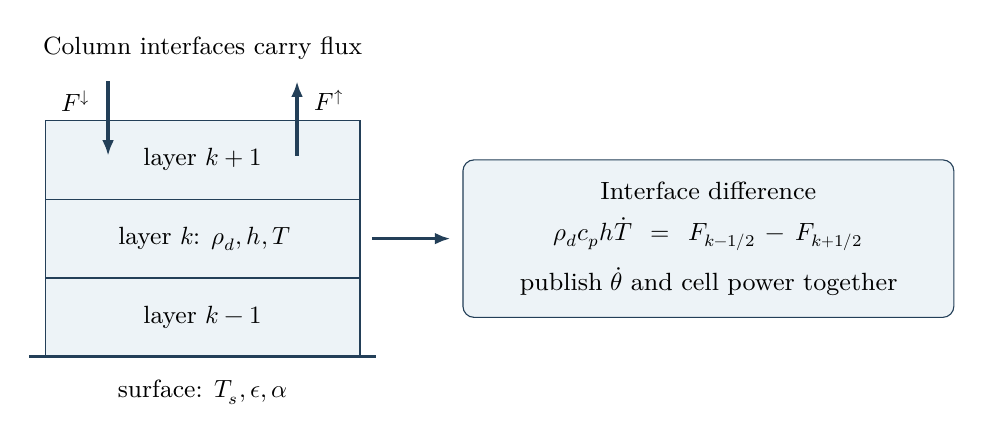
\begin{tikzpicture}[x=1cm,y=1cm,font=\small,
  ray/.style={-{Latex[length=2mm]},very thick,draw=NimbusBlue}]
  \draw[fill=NimbusLight,draw=NimbusBlue] (0,0) rectangle (4,3);
  \draw[draw=NimbusBlue] (0,1)--(4,1) (0,2)--(4,2);
  \node[above] at (2,3.65) {Column interfaces carry flux};
  \draw[ray] (.8,3.5)--(.8,2.55);
  \node[left] at (.7,3.25) {$F^\downarrow$};
  \draw[ray] (3.2,2.55)--(3.2,3.5);
  \node[right] at (3.3,3.25) {$F^\uparrow$};
  \node at (2,2.5) {layer $k+1$};
  \node at (2,1.5) {layer $k$: $\rho_d,h,T$};
  \node at (2,.5) {layer $k-1$};
  \draw[very thick,draw=NimbusBlue] (-.2,0)--(4.2,0);
  \node[below=5pt] at (2,0) {surface: $T_s,\epsilon,\alpha$};
  \draw[ray] (4.15,1.5)--(5.15,1.5);
  \node[draw=NimbusBlue,fill=NimbusLight,rounded corners,align=center,
        text width=6cm,minimum height=2cm,anchor=west] at (5.3,1.5)
    {Interface difference\\[4pt]
     $\rho_d c_p h\dot T=F_{k-1/2}-F_{k+1/2}$\\[5pt]
     publish $\dot\theta$ and cell power together};
\end{tikzpicture}
\caption{Upward-positive net flux is $F=F^\uparrow-F^\downarrow$.
The layer gains energy when more net power enters its lower face than leaves
its upper face. Summing layers cancels interior exchanges. Optical closure,
surface boundary conditions and physical layer mass remain separate assumptions.}
\end{figure}


The conversion supplied to the dynamics owner is
$\dot\theta=\dot T(p_{\rm ref}/p)^{R_d/c_p}$ using pressure at the evaluated
state. The later EOS projection still participates in the thermal path described
in the coupling chapter. Column power, temperature tendency and the stored
theta increment are related quantities, not interchangeable numerical arrays.
For a terrain cell, physical heights, interface geometry, volume and surface
area must retain their declared meaning before applying an analogous budget.

\section{Optical depth summarizes an interaction along a path}

At a frequency $\nu$, let $I_\nu(\boldsymbol x,\boldsymbol\Omega)$ be radiance
in direction $\boldsymbol\Omega$. A local, stationary transfer equation with
elastic scattering can be written schematically as
\[
 \boldsymbol\Omega\cdot\nabla I_\nu
 =-\beta_{e,\nu}I_\nu+\beta_{a,\nu}B_\nu(T)
 +\frac{\beta_{s,\nu}}{4\pi}
    \int_{4\pi}P_\nu(\boldsymbol\Omega,\boldsymbol\Omega')
                      I_\nu(\boldsymbol\Omega')\,d\Omega'.
\]
Absorption and scattering coefficients have units $\mathrm{m^{-1}}$;
$\beta_e=\beta_a+\beta_s$. This convention normalizes the phase function so
its angular integral is $4\pi$. The thermal term assumes local thermodynamic
equilibrium for the emitting material. A model that drops the scattering term
has made a different physical approximation from one that replaces its angular
integral with a quadrature.

For pure absorption along path coordinate $s$, optical depth is
$\tau=\int\beta_a\,ds$. With no emission on that path, the solution is
$I=I_0e^{-\tau}$. A vertical optical depth $\Delta\tau$ seen by a direct beam
with vertical cosine $\mu_0>0$ becomes path depth $\Delta\tau/\mu_0$ in a
plane-parallel layer. This geometric factor belongs to the beam direction.
A diffuse hemisphere contains many path angles and cannot generally use the
same single cosine.

Nimbus's schemes reduce spectral and angular detail in different ways. The
simple-grey scheme uses broadband optical depths. RRTMG uses spectral bands and
reduced absorption-distribution quadrature. The underlying transfer equations
help identify assumptions, but the code's quadrature, boundary rules and
coefficient inputs define the numerical calculation actually performed.

\section{The two simple-grey optical models}

The pressure-only clear-sky model defines an interface optical-depth profile
\[
 \tau(p)=\tau_{\rm ref}
       \left(\frac{p}{100000\,\mathrm{Pa}}\right)^n,
 \qquad\Delta\tau_k=\tau(p_{k-1/2})-\tau(p_{k+1/2}).
\]
Longwave and shortwave have separate reference depths and exponents. Pressure
interfaces must be finite, nonnegative and nonincreasing upward, with positive
surface pressure. This is a prescribed broadband profile, not a calculation
of molecular absorption from a complete gas spectrum. It deliberately provides
a simple radiative experiment whose parameters are model assumptions.

The absorbing water/cloud-path model adds absorber mass paths,
\[
 \Delta\tau_k^{\rm water}
 =\rho_{d,k}h_k
   \big(\kappa_vq_{v,k}+\kappa_lq_{c,k}+\kappa_iq_{i,k}\big).
\]
The mass-absorption coefficients $\kappa_x$ have units
$\mathrm{m^2\,kg^{-1}}$, so the expression is dimensionless. Separate
coefficients are supplied for the two broadband components. This path uses
vapor, cloud liquid and cloud ice. It does not automatically turn rain, snow,
graupel or hail into optical contributors merely because those categories
exist in microphysics.

The absorbing model adds this term to the pressure-profile layer depth. It is
not a scattering cloud model: changing cloud water changes absorption, but
does not create the cloud scattering and angular redistribution represented by
a more elaborate optical scheme. Configuration must pair the selected optical
model with its clear-sky setting consistently. The
\href{../src/radiation/schemes/simple_grey/simple_grey.cpp}{simple-grey owner}
validates those choices and requires physical column inputs.

\section{Grey longwave transfer and the surface boundary}

The implemented longwave calculation treats each layer as isothermal for its
broadband source. With $\mathcal T_k=e^{-\Delta\tau_k}$, it uses recurrences
of the form
\[
 \begin{aligned}
 F^\downarrow_{k-1/2}
 &=\mathcal T_k F^\downarrow_{k+1/2}
   +(1-\mathcal T_k)\sigma T_k^4,\\
 F^\uparrow_{k+1/2}
 &=\mathcal T_k F^\uparrow_{k-1/2}
   +(1-\mathcal T_k)\sigma T_k^4.
 \end{aligned}
\]
These equations describe the code's effective optical-depth convention; no
additional longwave diffusivity factor should be inserted when reproducing this
particular grey calculation. They assume a broadband thermal source and neglect
longwave scattering in this path.

The top incoming longwave flux is zero. After the downward sweep reaches the
surface, the upward lower boundary is
\[
 F^\uparrow_s=\epsilon\sigma T_s^4
                 +(1-\epsilon)F^\downarrow_s.
\]
The second term represents reflected downwelling longwave. Omitting it would
make a nonblack surface absorb energy that its declared emissivity does not
permit under this opaque-surface convention. The upward sweep therefore depends
on the completed downward sweep. Surface temperature and emissivity are explicit
inputs; the radiation calculation does not solve a soil or land-surface energy
balance that prognoses a new $T_s$.

The recurrences and the flux-divergence conversion are separate stages in
\href{../src/radiation/base/radiative_transfer.cpp}{radiative transfer}.
A valid recurrence can still produce the wrong heating if layer indexing,
interface orientation or the mass used by the conversion is inconsistent.

\section{Direct sunlight and Lambertian reflection are different angular fields}

For an illuminated flat column, the top incident shortwave flux is
$F^\downarrow_{\rm top}=\mu_0 S_0$, where $S_0$ is irradiance normal to the
solar beam. The downward grey path attenuates each layer by
$e^{-\Delta\tau_k/\mu_0}$. The nighttime branch publishes no shortwave source
rather than evaluating a singular or negative path length at $\mu_0\le0$.

At the surface, the reflected upward flux is
$F^\uparrow_s=\alpha F^\downarrow_s$. Nimbus treats this reflected boundary
as Lambertian. Its radiance is direction-independent over the upward hemisphere,
so the upward flux at cumulative optical depth $\tau$ above the surface is
\[
 F^\uparrow(\tau)=F^\uparrow_s\,2E_3(\tau),\qquad
 E_3(\tau)=\int_1^\infty\frac{e^{-\tau t}}{t^3}\,dt.
\]
The factor follows directly from hemispheric integration:
$2\int_0^1\mu e^{-\tau/\mu}\,d\mu=2E_3(\tau)$.
It approaches one at zero optical depth. Applying the direct solar cosine to
this reflected flux would give it the wrong angular distribution.

This grey construction contains atmospheric absorption and a reflecting lower
boundary but no atmospheric scattering. Albedo changes the energy partition
between the surface and the upward radiation; it is not a source of energy.
The implementation evaluates the exponential-integral transmission with bounded
numerical branches and rejects nonphysical results. Tests of the thin, thick,
black-surface and reflecting-surface limits examine different parts of this
contract.

\section{What the correlated-k approximation changes}

Molecular absorption varies rapidly with frequency. Resolving every spectral
line in every grid column would be expensive. Within a band, an absorption
coefficient distribution can be represented by a cumulative variable $g$,
turning a band transmission integral into an approximation such as
\[
 \overline{\mathcal T}(u)
 =\int_0^1e^{-k(g)u}\,dg
 \simeq\sum_j w_j e^{-k_j u}.
\]
Here $u$ is the absorber amount in the coefficient convention and the weights
cover the distribution interval. Using correlated ordering between layers,
combining gases and interpolating coefficients across temperature and pressure
introduce additional modeling assumptions. This is a spectral quadrature;
its $g$ coordinate is not gravitational acceleration or a particle-size moment.

\href{https://doi.org/10.1029/97JD00237}{Mlawer et al. (1997)} develops the
longwave correlated-k reference method, and
\href{https://doi.org/10.1029/2008JD009944}{Iacono et al. (2008)} describes the
AER model family and its greenhouse-gas forcing calculations. Their validation
results do not automatically apply to Nimbus's translated implementation,
coefficient versions, cloud assumptions or coupled runtime.

Nimbus implements the calculation in C++; the AER netCDF files provide
coefficients rather than an executable Fortran solver. Typed loading validates
the expected coefficient schema and identity. Pressure/temperature preparation,
major and minor gas absorption, continua, cloud optics and transfer have
separate source owners under
\href{../src/radiation/schemes/rrtmg/}{the RRTMG implementation}. The reduced
spectral structure is part of those coefficient contracts, not a tunable number
of arbitrary equal-frequency samples.

\section{Gas columns, cloud optical properties and transfer closure}

Nimbus constructs dry-air molecular columns from the supplied dry density and
physical layer thickness. With dry molar mass $M_d$ in $\mathrm{kg\,mol^{-1}}$,
\[
 N_d=\frac{\rho_d h}{M_d}\,\frac{N_A}{10^4}
\]
gives molecules per square centimetre. A water dry-air mass mixing ratio is
converted to a dry-air-relative molar ratio with
$r_v=q_v M_d/M_v$. Gas mole fractions and their allowed totals have explicit
validation. Pressure, temperature and molecular column amounts therefore have
different roles; substituting a pressure-thickness formula for the actual
$\rho_d h$ preparation without reviewing its assumptions changes the inputs.

The runtime currently passes cloud liquid $q_c$ and cloud ice $q_i$ to the
optics. In cloudy mode it uses liquid/ice mass paths
$1000\rho_d h q_c$ and $1000\rho_d h q_i$ in $\mathrm{g\,m^{-2}}$, with
configured effective radii in micrometres. A cell with either positive cloud
category is assigned cloud fraction one; otherwise it is clear. There is no
prognostic subgrid cloud fraction or general cloud-overlap model in this
construction. Effective radii are optical inputs here, not automatically the
radius diagnosed from every microphysics moment. Falling condensate categories
are not silently summed into the two cloud paths.

Longwave transfer includes its band-dependent diffusivity treatment. Shortwave
transfer uses the implemented practical improved flux method (PIFM) two-stream
layer coefficients, direct/diffuse reflection and transmission, and the
supplied scattering/asymmetry information. A two-stream solution represents an
angular closure, not the full radiance field at every direction. Conservative
scattering and optically thin limits need stable numerical branches because
algebraically equivalent expressions can suffer cancellation or singular-looking
intermediate terms. See
\href{../src/radiation/schemes/rrtmg/rrtmg_longwave_transfer.cpp}{longwave transfer}
and \href{../src/radiation/schemes/rrtmg/rrtmg_shortwave_transfer.cpp}{shortwave transfer}.

Interface temperatures, when not supplied, use the retained pressure-coordinate
interpolation and endpoint rules. The physical column order and the transfer
solver's sweep order are explicitly converted. Agreement of a single surface
flux does not establish that all interface fluxes, layer heating and cloud/gas
responses agree with an independent column reference.

\section{Terrain adds visibility, projected area and horizontal exchange}

For a unit direction toward the Sun, $\boldsymbol s$, and an upward surface
normal $\boldsymbol n$, direct intercepted irradiance is proportional to
$\max(0,\boldsymbol n\cdot\boldsymbol s)$. Visibility is an additional condition:
a face aimed toward the Sun may still be shadowed by intervening terrain.
Area measured along the slope differs from horizontal plan area. Fluxes in
$\mathrm{W\,m^{-2}}$ must be paired with the area their definition uses before
becoming power in watts.

Nimbus has explicit terrain shortwave paths for visibility, ray traversal,
absorbed power, reflected angular transport and spectral variants. A ray through
several physical cells carries an energy amount; attenuation along each segment
partitions it between absorption and outgoing power. A reflecting terrain
boundary can redirect it into other columns. Reusing independent vertical-column
heating while merely shading a picture would not represent that exchange.

For a bounded shortwave transport calculation, an appropriate whole-domain
partition is
\[
 P_{\rm in}=P_{\rm atmosphere}+P_{\rm surface}
        +P_{\rm top\ escape}+P_{\rm lateral\ escape}+P_{\rm unresolved}.
\]
The unresolved term records power remaining when a declared angular/bounce or
convergence bound is reached; it is not automatically atmospheric heating.
Changing quadrature, reflection count or stopping tolerance changes a numerical
approximation that must be checked independently of this bookkeeping identity.

Source presence does not imply every terrain/backend combination is admitted.
The current runtime rejects mapped RRTMG shortwave on an active accelerator
because its native spectral-terrain owner is missing. CPU mapped spectral work
and native column batches have separate scopes. The
\href{../src/radiation/runtime.cpp}{radiation runtime} is the authority for the
actual selected path and required rejection behavior.

\section{Cadence, stored power and the complete coupled step}

Radiation is refreshed on its declared cadence and can hold its source between
calls. The evaluated optical state, published heating and held power must share
one completed generation. The next dynamics interval should not combine a newly
computed power diagnostic with an older held theta tendency. A refresh failure
must preserve the preceding coherent runtime state and its timing.

If a held atmospheric power is $P_h$ over an interval $\Delta t$, its declared
energy input is $P_h\Delta t$. The
\href{../src/radiation/energy_ledger.cpp}{radiation energy ledger} accounts for
that held input and the relevant source endpoint. This is distinct from simply
recomputing an interface-flux difference from a later atmospheric column.
Cadence holding approximates time evolution; a smaller dynamics step does not
by itself make a long-held radiation source current.

The checks in \href{../tests/physics/test_radiation.cpp}{radiation tests} and
\href{../tests/physics/test_radiation_runtime_state.cpp}{runtime-state tests}
cover columns, units, invalid inputs, closure and publication behavior for their
stated scopes. Broader coupled, terrain, restart and native paths need their own
bounded and campaign evidence. Neither a familiar scheme name nor a finite
flux residual replaces that validation.


\chapter{Unresolved mixing, stochastic forcing and diagnostic interpretation}
\label{mixing-theory}

The resolved equations do not describe every turbulent eddy, surface exchange
or particle-scattering process inside a cell. Closures supply those missing
relationships. They are mathematical models with their own state, scales and
admissible inputs, not interchangeable corrections to a finished solution.
This chapter follows the implemented Nimbus closures and their connections to
transport and diagnostics. The earlier grid and microphysics chapters supply
the carrier and moment conventions; the architecture guide explains the
corresponding state and execution owners.

\section{Eddy viscosity connects resolved strain to unresolved transport}

For physical Cartesian velocity components, define the symmetric strain
$S_{ij}=\tfrac12(\partial_j u_i+\partial_i u_j)$ and its magnitude
$|S|=(2S_{ij}S_{ij})^{1/2}$. Strain has units s$^{-1}$. An eddy viscosity
models an unresolved momentum exchange through a stress proportional to
resolved deformation. A viscous-traction form is $\tau_{ij}=2\rho_d\nu_tS_{ij}$,
with acceleration from its divergence divided by the appropriate carrier.
This motivates the closure; its isotropic/compressional and directional
treatment must still follow the actual discrete tensor owner.

Static Smagorinsky uses
\[
 \nu_t=(C_s\Delta)^2|S|,\qquad
 K_\theta=\nu_t/\mathrm{Pr}_t,\qquad
 K_q=\nu_t/\mathrm{Sc}_t.
\]
Here $C_s$ is dimensionless, $\Delta$ is a length, and viscosity/diffusivities
are in m$^2$ s$^{-1}$. Nimbus additionally applies configured coefficient
bounds and the selected stability correction. Increasing $C_s$ or the filter
length increases modeled mixing; it is not equivalent to changing a plotting
resolution. The retained \texttt{dx} filter option actually uses
$\sqrt{\Delta x\Delta y}$, while \texttt{cubic\_root} uses
$(\Delta x\Delta y\Delta z)^{1/3}$. A user filter is a prescribed physical
length. Mapped filters use the horizontal footprint and physical Jacobian
thickness, not a sloping face-normal CFL distance.

Directional modes select which gradients and exchanges participate. In the
flat derivative limit, the strain measures have the forms
\[
\begin{aligned}
 |S|_h^2&=2(S_{xx}^2+S_{yy}^2)+4S_{xy}^2
                    +(\partial_xw)^2+(\partial_yw)^2,\\
 |S|_v^2&=(\partial_zu)^2+(\partial_zv)^2+2S_{zz}^2.
\end{aligned}
\]
The horizontal-only mode therefore retains horizontal gradients of vertical
velocity. It is not simply a two-component two-dimensional atmosphere.
The C-grid implementation averages appropriate edge contributions; averaging
a gradient before squaring is generally different from averaging its square.
These choices are explicit in
\href{../src/turbulence/base/eddy_viscosity.cpp}{the shared SGS operators}.

For example, two neighboring shear samples $+a$ and $-a$ have a zero mean but
a mean square $a^2$. A closure that first averages them and then squares would
diagnose no deformation contribution at all. This is why matching array sizes
does not justify changing the staggered averaging order. The physical
interpretation is also limited: eddy viscosity parameterizes unresolved
transport at a filter scale; it is not molecular viscosity and does not
resolve the omitted eddies. Refining the grid while retaining a grid-derived
$\Delta$ changes both the resolved field and its unresolved closure.

Stable stratification can suppress turbulence. With the declared buoyancy
frequency squared $N^2$, the versioned Lilly-equilibrium branch uses a strain
factor equivalent to
\[
 |S|_{\mathrm{eff}}=
 \sqrt{\max(0,|S|^2-N^2/\mathrm{Pr}_t)}.
\]
Positive $N^2$ reduces mixing; negative $N^2$ increases the available scale.
Nimbus evaluates the expression with separate stable/unstable numerical forms
and retains a distinct older Richardson-correction option. Those options must
not be called identical. Moist versus dry buoyancy, coefficient caps and the
selected directional mode are part of the closure contract. The static
vertical-only tracked scope remains Engineering incomplete; the presence of
these formulas does not authorize every PBL, terrain or accelerator combination.

\section{Dynamic Smagorinsky diagnoses a bounded coefficient}

A dynamic model uses information at a second filter scale rather than prescribing
one coefficient everywhere. Nimbus reconstructs scalar-center fields, applies
a density-weighted Favre test filter and forms a resolved stress difference
$L_{ij}$ and a model difference $M_{ij}$. With a local least-squares assumption,
the coefficient multiplying the grid-scale model is estimated from their
contraction. The retained implementation averages horizontally at each height:
\[
 C(k)=\operatorname{clip}\!\left(
 \frac{\sum_{i,j}L_{ab}M_{ab}}{\sum_{i,j}M_{ab}M_{ab}},
 0,C_{s,\max}^2\right),\qquad C_s(k)=\sqrt{C(k)}.
\]
Repeated tensor indices denote the symmetric-tensor contraction, including
off-diagonal contributions. If the denominator is too small, the coefficient
is zero. The nonnegative bound excludes SGS backscatter in this implementation;
it is a deliberate model restriction, not a general theorem about turbulence.

The test width is twice the grid filter width. Favre filtering uses
$\widehat{\rho_d\phi}/\widehat{\rho_d}$, so ordinary averaging is not an
equivalent replacement in a variable-density field. Horizontal periodic
wrapping and bounded vertical sampling are also part of the retained filter.
The current owner requires its flat, periodic, C-grid, 3-D CPU domain and
rejects a required-native request. It is not a generic dynamic model for all
boundaries or mapped geometries. See
\href{../src/turbulence/schemes/smagorinsky/dynamic_smagorinsky.cpp}{dynamic
coefficient construction} and
\href{../tests/physics/test_turbulence_sgs.cpp}{SGS reference tests}.

Horizontal averaging is a substantive assumption. It supplies one coefficient
for a height plane and suppresses fluctuations in the least-squares ratio,
but can blend a strongly sheared storm core with a quieter environment. A
pointwise or Lagrangian average would define a different model, not simply a
faster reduction. The current test filter has separable three-point weights
$(1/4,1/2,1/4)$; its finite vertical edge treatment is distinct from a periodic
three-dimensional filter. The dynamic branch also rejects a separately
selected stability correction rather than composing two coefficient models
without a declared derivation.

\section{Prognostic TKE supplies a second modeled energy reservoir}

Let $e$ denote unresolved turbulent kinetic energy per unit dry mass, with units
m$^2$ s$^{-2}$. Its closure has the schematic material form
\[
 \frac{De}{Dt}=P_s+P_b-\epsilon
       +\frac{1}{\rho_d}\nabla\!\cdot(\rho_dK_e\nabla e).
\]
Shear production transfers energy through deformation; buoyancy production can
create or suppress turbulence; dissipation removes modeled TKE. Resolved
advection and source application still belong to the coupled timestep. A TKE
equation alone does not establish a conservative exchange with resolved kinetic
or internal energy.

Nimbus's Deardorff--Moeng-style branch uses $\nu_t=0.1\ell\sqrt e$. With its
stability correction active, the stable mixing length is limited by
$\ell=\min(\Delta,0.76\sqrt e/N)$ for $N>0$; neutral/unstable conditions use
the grid length, and disabling the correction retains that length directly.
For positive $e$, its retained dissipation is
\[
 \epsilon=\left(0.19+0.51\frac{\ell}{\Delta}\right)
             \frac{e^{3/2}}{\ell}.
\]
The zero-energy case has its own zero-source treatment. This avoids interpreting
the displayed quotient as permission to divide by a vanished length.

Scalar transport also depends on the length ratio. Before configured caps,
\[
\begin{aligned}
 K_\theta&=\nu_t\left[1+
        (\mathrm{Pr}_t^{-1}-1)\ell/\Delta\right],\\
 K_q&=\nu_t\left[1+
        (\mathrm{Sc}_t^{-1}-1)\ell/\Delta\right],\qquad K_e=2\nu_t.
\end{aligned}
\]
Thus replacing all three by one diffusivity changes the closure. Stress work,
TKE production and scalar diffusion use physical geometry and the admitted
discrete locations. The
\href{../src/turbulence/schemes/tke/tke.cpp}{TKE source} and
\href{../tests/physics/test_tke_scheme.cpp}{tests} define the actual branch,
including finite input, positivity and native-path requirements.

The stable length has the expected dimensions: $\sqrt e$ is a velocity and
$N$ an inverse time, so their ratio is a length. As stability reduces
$\ell/\Delta$, the scalar-to-momentum ratios above approach one. This is
different from applying a constant Prandtl number after computing viscosity.
The dissipation coefficient also varies with the length ratio, so changing
only the viscosity length would leave an inconsistent closure. Whether the
removed TKE is returned to another represented energy reservoir must be checked
in the actual coupled source/energy owner; the sign of $\epsilon$ alone does
not prove that exchange is implemented conservatively.

\section{PBL columns and surface exchange operate at another modeling scale}

The PBL choices are none, slab, YSU and MYNN. None supplies no PBL forcing; it
does not disable separately selected resolved-grid SGS. Active PBL models
represent vertical column transport and surface exchange with different
assumptions from a three-dimensional LES stress. Combining them requires an
explicit division of transport to avoid counting the same unresolved exchange
twice.

A useful column notation makes the nonlocal assumption visible:
\[
 J_\phi=-\rho_dK_\phi(\partial_z\phi-\gamma_\phi)
              +J_{\phi,\mathrm{entrainment}}.
\]
$\gamma_\phi$ has the units of a vertical gradient. For theta, $J_\theta$
has units kg K m$^{-2}$ s$^{-1}$ and still needs the declared heat conversion
to become W m$^{-2}$. For a water mixing ratio, the analogous flux is a water
mass flux. A positive countergradient contribution can transport a scalar
against its local gradient because it represents nonlocal eddies. Consequently,
one cannot infer the complete flux sign from $K>0$ alone. This schematic form
organizes the coupling; each PBL family supplies its own terms and limits.

The slab owner retains a mixed-layer state and diagnoses a bounded depth $h$.
Its column heights are measured above local ground. Weighting respects partial
layer overlap:
\[
 m_k=\rho_{d,k}\max\!\left(0,
       \min(h,z_{k+1/2})-z_{k-1/2}\right),\qquad
 \overline\phi_m=\frac{\sum_km_k\phi_k}{\sum_km_k}.
\]
These are masses per horizontal area. Mixing and surface forcing are applied
using complete cell masses so a partly occupied top layer does not receive a
full layer's forcing. Stored mixed-layer quantities and realized fluxes must
remain consistent with the resolved column. The word slab here does not imply
a prognostic soil reservoir. See
\href{../src/boundary_layer/schemes/slab/slab.cpp}{slab mixing}.

YSU supplies nonlocal transport and explicit entrainment, with physical
background in
\href{https://journals.ametsoc.org/view/journals/mwre/134/9/mwr3199.1.xml}{Hong,
Noh and Dudhia (2006)}. Nimbus's interior diffusivity profile has the
characteristic $K\sim\kappa w_m z(1-z/h)^2$ structure before its stability and
bounding choices. A scalar flux contains a downgradient part and, where
selected, a countergradient correction; entrainment adds a distinct top
exchange. The implemented temperature, moisture and momentum terms are not
all identical: for example, its moisture flux does not simply reuse the
temperature countergradient term. The
\href{../src/boundary_layer/schemes/ysu/ysu.cpp}{retained YSU owner} determines
the exact coefficients and interval solve.

MYNN uses prognostic TKE and stability functions, with background in
\href{https://www.jstage.jst.go.jp/article/jmsj/87/5/87_5_895/_article/-char/en}{Nakanishi
and Niino (2009)}. In Nimbus's level-2.5 notation, $q^2=2e$ is a velocity-variance
quantity, not water mixing ratio. The diffusivities have the form
\[
 K_m=\ell\sqrt{2e}\,S_m,
 \qquad K_h=\ell\sqrt{2e}\,S_h,
\]
with stability functions depending on shear, buoyancy and the mixing-length/TKE
state. The retained Helfand--Labraga correction limits unrealizable states;
invalid denominators or coefficients reject rather than silently producing
an arbitrary mixing rate. MYNN's column TKE is a closure state with its own
solve, not permission to add an independent LES TKE source twice. See
\href{../src/boundary_layer/schemes/mynn/mynn.cpp}{MYNN} and
\href{../src/boundary_layer/schemes/mynn/mynn_stability.cpp}{stability functions}.

\section{Surface-flux signs, units and prescribed skin state}

Let $\boldsymbol U$ be near-surface air velocity relative to the physical
surface, $U=|\boldsymbol U|$, and $\Pi=(p/p_{\rm ref})^{R_d/c_{pd}}$.
The retained bulk exchange takes the form
\[
\begin{aligned}
 \boldsymbol\tau&=-\rho_dC_dU\boldsymbol U,\\
 H&=\rho_dc_{pd}\Pi C_hU(\theta_s-\theta_a),\\
 E&=\rho_dC_eU(q_s-q_a).
\end{aligned}
\]
Stress opposes relative air motion; positive $H$ heats the atmosphere and
positive $E$ supplies vapor. Their units are N m$^{-2}$, W m$^{-2}$ and
kg m$^{-2}$ s$^{-1}$ respectively. $L_vE$ is a latent-energy flux, whereas $E$
itself is not. The Exner factor in $H$ converts a potential-temperature flux
to sensible-heat currency; omitting it changes the implemented exchange.

Neutral coefficients use separate momentum and heat roughnesses:
\[
 C_{d0}=\frac{\kappa^2}{\ln^2(z/z_{0m})},\qquad
 C_{h0}=\frac{\kappa^2}{\ln(z/z_{0m})\ln(z/z_{0h})}.
\]
The bulk branch applies retained Louis stability factors. The Monin--Obukhov
branch instead iterates stability-corrected logarithmic denominators using
$\zeta=z/L$ and the surface virtual-potential-temperature flux:
\[
 L=-\frac{u_*^3\theta_{v,a}}
          {\kappa g\,\overline{w'\theta_v'}_s},\qquad
 \overline{w'\theta_v'}_s\simeq
 \frac{H}{\rho_dc_{pd}\Pi}+0.61\theta_a\frac{E}{\rho_d}.
\]
An unstable positive virtual heat flux therefore gives negative $L$. Nimbus
retains explicit neutral limits, iteration limits and minimum-friction-velocity
handling; these are part of the algorithm, not an unbounded analytic law.

The minimum-$u_*$ treatment can increase momentum and heat/moisture transfer
coefficients together. It is therefore a modification of the exchange, not a
harmless display floor. Roughness must be below the reference sampling height,
and the neutral limit must remain finite. These checks are necessary even for
a flat surface: a logarithmic formula evaluated outside its geometric domain
does not become physical by clipping its final flux afterward.

Skin temperature and moisture are prescribed, or initialized from the initial
surface air when unset and subsequently held. There is no prognostic soil
heat/moisture or vegetation model behind them. On sloping ground, tangent wind,
traction and actual-versus-horizontal area must be transformed consistently.
See \href{../src/boundary_layer/base/surface_fluxes.cpp}{surface exchange}.
Neither radiative surface absorption nor a surface-flux receipt automatically
evolves a land temperature that the model does not own.

\section{Diffusion applies a closure; it does not define one}

The density-weighted scalar diffusion form is
$\rho_d\partial_t\phi=\nabla\!\cdot(\rho_dK\nabla\phi)$.
The coefficient can come from a prescribed numerical profile or a physical
closure. Explicit time integration has a diffusion stability restriction;
implicit vertical exchange solves a coupled column system over the interval.
Neither method makes an inappropriate coefficient physically justified.

Nimbus separates coefficient construction, transport/application and realized
source reports. An implicit solve's accepted flux need not equal an explicit
flux formed from the old gradient. PBL held sources retain interval-mean
forces and inventory rates so changing density does not accidentally reuse a
stale acceleration denominator. Momentum diffusion also changes resolved
kinetic energy, with a finite-step contribution beyond linear work. Appropriate
boundary work and TKE/thermal attribution must be assessed together.
The existing diffusion chapter derives the spatial and temporal operators;
the closure-specific question is which $K$, carrier, interval and coupled
energy owner feed them.

Some admitted paths defer transport-tendency construction until the selected
application owner consumes closure coefficients. That prevents an explicit
tendency from being applied and then implicitly applied again over the same
interval. It also makes coefficient lifetime significant: a matrix built from
one state is not automatically the matrix corresponding to a later gradient
or density. Changes between explicit, implicit and deferred paths need tests
of the accepted state and realized flux, including rejection, rather than a
comparison of coefficient arrays alone.

\section{Stochastic perturbations have covariance and conservation contracts}
\label{chaos-theory}

The chaos choices are none, initial-condition perturbations, boundary-layer
perturbations and full stochastic coupling. A simple temporal building block
is the retained AR(1) update
\[
 \xi_{n+1}=a\xi_n+\sqrt{1-a^2}\,\eta_n,
 \qquad a=\exp(-\Delta t/\tau).
\]
If independent innovations $\eta_n$ and the previous field each have zero mean
and unit variance, the new variance is $a^2+(1-a^2)=1$. That explains the
innovation coefficient. Finite-grid normalization, spatial filtering,
clipping and conditioning can change the realized distribution. The variance
identity does not establish the exact finite-domain distribution after those
additional transformations. The actual noise refresh interval must
be used; replacing it with an unrelated solver step changes decorrelation.

The spectral spatial filter multiplies Fourier components by
\[
 G(k_x,k_y)=\exp[-\tfrac12\{(L_xk_x)^2+(L_yk_y)^2\}].
\]
This attenuates short scales. The recursive alternative applies repeated
forward/backward smoothing with weights such as $\exp(-\Delta x/L_x)$.
It approximates a correlated field through a different discrete operation;
it is not identical to the spectral filter. Filter widths, boundary treatment
and variance normalization affect the resulting covariance. A configured
length is not automatically the measured autocorrelation length of every
clipped or relocated field. See
\href{../src/chaos/base/correlation_filter.cpp}{correlation filters} and
\href{../src/chaos/base/perturbation_field.cpp}{temporal updates}.

Seeds are combined with member, process/field and sequence identity. Restart
must preserve the retained noise generation and clock. Earth-correlated noise
uses its declared physical control-grid coordinates; a translated window must
not invent a new forcing realization solely because an Earth point acquires
a different array index. Different standard-library random-distribution
implementations are not automatically bitwise equivalent despite equal seeds.

A source multiplier of the form $1+\alpha\xi$, subject to the declared bounds,
changes a process. It must be applied to the associated transfers or conserved
column exchange consistently. Scaling water tendencies independently can break
their zero sum; scaling a sedimentation divergence without its lower-boundary
flux breaks precipitation accounting. Nimbus retains source/column ownership
and private-state checks for admitted stochastic couplings. The current
\href{../src/chaos/schemes/full_stochastic/full_stochastic.cpp}{full-stochastic
owner} is not a license to multiply every physical term by unrelated noise.
Ensemble spread is also not calibrated forecast uncertainty merely because
the perturbation variance is known.

Bounding a multiplier also changes its statistics: even if $\xi$ has zero mean,
the mean of a clipped $1+\alpha\xi$ need not be exactly one. Common process
identity and a conserved-transfer construction address a different question
from unbiased ensemble forcing; neither follows automatically from the AR(1)
variance calculation.

\section{Radar products are bulk forward operators}
\label{radar-diagnostics-theory}

Radar diagnostics translate modeled particles and wind into an observation-like
quantity. A Rayleigh liquid reference motivates the sixth-diameter moment
$Z=\int D^6n_v(D)\,dD$, with a volume spectrum and conversion to
mm$^6$ m$^{-3}$. Its logarithmic form is
\[
 Z_{\rm dBZ}=10\log_{10}\!\left(
       Z_e/(1\ \mathrm{mm^6\,m^{-3}})\right).
\]
Frozen-particle density, dielectric behavior and shape require further
assumptions. Summing component reflectivities must occur in linear space,
not by adding their dBZ values.

Nimbus's \texttt{fast\_da} and \texttt{psd\_moment} tiers retain concrete
bulk relationships. Without supplied number, a species path uses
$Z_{e,x}=A_x(\rho_dq_x)^{1.75}$. With supplied number, its moment proxy has
the form $Z_{e,x}=C_x(\rho_dq_x)^2/N_{v,x}$ with retained species factors.
The number used by that interface is interpreted per volume; a private number
per kg dry air needs conversion before being supplied. The tier can use the
mass-only relation when the corresponding number is absent. These are retained
proxies, not an arbitrary gamma-spectrum integral or a general electromagnetic
scattering solver. See
\href{../src/radar/schemes/reflectivity/reflectivity.cpp}{reflectivity tiers}.

Radial velocity projects reconstructed physical wind onto the vector from the
radar to the sample:
$V_r=\boldsymbol u\cdot\widehat{\boldsymbol r}$, with the configured bulk
scatterer fall correction when selected. C-grid face winds are reconstructed
at the declared scalar sample before projection. Terrain heights and Earth
origin determine the line of sight. The current \texttt{beam\_volume} option
uses a bounded local neighborhood average; it is not a complete antenna beam,
pulse-volume, attenuation or instrument-noise simulator. The
\href{../src/radar/schemes/velocity/velocity.cpp}{velocity owner} defines its
sampling and fall-speed bounds.

Differential reflectivity is $Z_{DR}=10\log_{10}(Z_H/Z_V)$ where the signals
are valid. Nimbus retains \texttt{simple}, \texttt{polarimetric\_fo} and
\texttt{zhang2021\_rain\_mp} paths. The bulk polarimetric path uses prescribed
shape/species relationships and publishes associated KDP and correlation
products within declared ranges; its name does not establish a T-matrix
calculation. The separate rain-MP path rejects frozen-species participation.
KDP is expressed in degrees per kilometre and the correlation coefficient is
dimensionless; these units do not make a bulk proxy a resolved beam-phase model.
Low/no-signal conventions and clipping are part of output interpretation.
The \href{../src/radar/schemes/zdr/zdr.cpp}{polarimetric source} and its tests
must accompany any claim about an admitted product set.

\section{Diagnostic integrals, storm objects and parcel paths}

Budget diagnostics integrate physical inventories and boundary exchanges,
using their versioned dry/mixture mass and phase-reference conventions. An
exact telescoping ledger records how a diagnostic changed; independent source,
work and boundary references are still needed to validate its physics.
Derived gradients and layer integrals require physical heights and finite
coverage, not a nominal index range.

The sounding diagnostic lifts a surface parcel dry-adiabatically to its LCL
and with a retained moist lapse-rate approximation above it. Vapor-corrected
virtual temperatures give buoyancy
$B=g(T_{v,p}-T_{v,e})/T_{v,e}$. Its CAPE is the positive buoyancy integral
between diagnosed LFC and EL; CIN is reported as a nonnegative magnitude of
the negative integral below LFC. Nimbus uses discrete layer integration and
finite column coverage. With no LFC it reports unavailable crossing heights
and a no-LFC interpretation with zero CIN, not evidence that inhibition is
physically absent. A top-limited EL likewise needs its finite-column context.
See \href{../src/init/sounding/diagnostics.cpp}{sounding diagnostics}.

Storm detection uses resolved updraft, condensate and rotation evidence to form
feature candidates. Temporal association, branching and ambiguity rules select
a track rather than identifying a uniquely defined physical object from one
maximum. Updraft helicity has the dimensional form $\int w\zeta\,dz$ over its
declared updraft/height support; storm-relative helicity uses the signed
storm-relative hodograph convention. Their values depend on physical layer
coverage and the selected storm motion. The
\href{../src/diagnostics/storm_tracker.cpp}{tracker} retains history because
continuity cannot be reconstructed from a single frame.

Air-parcel trajectories solve $d\boldsymbol x/dt=\boldsymbol u(\boldsymbol x,t)$
under the model's interpolation and frame assumptions. Nimbus prepares a
predicted midpoint from the beginning wind, samples there, and combines that
midpoint sample with the end-state midpoint wind during completion. This
differs from a streamline in one frozen velocity field. Stagger-aware sampling,
physical height, vertical clamping, horizontal departure and Earth-frame output
are explicit choices; the paths are not inertial precipitation trajectories.
\href{../src/diagnostics/trajectories/trajectories.cpp}{Trajectory continuation}
retains parcels and sample cadence through restart and movement.

These diagnostics test different aspects of a simulation. Matching rainfall,
CAPE or a storm track does not uniquely validate all closures that produced
them. Bounded formula, coupling and failure checks establish their stated
implementation scope; long campaigns and independent scientific review remain
separate from those checks.


\chapter{Putting it all together: one atmosphere, one timestep}\label{putting-it-together}

The preceding chapters describe individual equations and numerical choices.
A simulation becomes coherent only when those choices describe the same air,
water, geometry and time interval. This chapter follows a complete update and
shows how to reason about its coupled behavior. The main example is the
Cartesian C-grid split-explicit path with bulk microphysics. Other admitted
integrators and geometries have their own stage owners; the example is not a
claim that one ordering can be substituted for every supported configuration.

\section{Begin with a complete mathematical state}

A useful abstract state is
\[
 X=(\rho_d,\theta,\boldsymbol u,\boldsymbol q,\boldsymbol N,
       \boldsymbol Z,\boldsymbol s,\mathcal G,\mathcal H).
\]
Here $\boldsymbol q$ contains the selected water species, $\boldsymbol N$
contains the applicable number concentrations, and $\boldsymbol Z$ denotes
additional prognostic moments only where a scheme actually owns them.
$\boldsymbol s$ includes scheme-private physical state such as held column
sources or turbulence variables. $\mathcal G$ is geometry and domain placement;
$\mathcal H$ includes histories needed by boundaries, staged integration and
continuation. Some of these components are absent for a simpler configuration.
Pressure is additionally stored and used, but its committed relationship to
dry density and potential temperature is constrained by the production EOS.

The state is larger than the arrays shown in a plot. Two runs with identical
visible temperature and water at one instant can evolve differently if their
particle number, held heating interval, radiative boundary history or nested
placement differs. A restart specification must therefore identify the full
continuation state. A snapshot of plotted fields is insufficient evidence that
the next tendency will match.

Geometry is included because changing cell volume changes the interpretation
of density and mixing ratio. Time history is included because a source held
between radiation calls is not equivalent to a source freshly evaluated from
the current cloud. A complete state definition is the first defense against
accidentally comparing different mathematical problems while believing that
only a backend, thread count or file format changed.

\section{Initialization must create a mutually compatible state}

A sounding supplies a vertical environment, but the solver must place it on
its own scalar and velocity locations. The procedure needs physical heights,
a pressure/base-state construction, water conventions and an equation of state.
An interpolation that is monotone in a sounding coordinate does not
necessarily preserve hydrostatic balance on the model interfaces. Similarly,
using moisture in a thermodynamic conversion does not justify adding it a
second time to a buoyancy correction.

For a simple resting dry column, hydrostatic balance is
$dp_0/dz=-\rho_0g$. A discrete balance might be expressed at a face as
\[
 \frac{p_{0,k+1}-p_{0,k}}{z_{k+1}-z_k}
 =-g\rho_{0,k+1/2},
\]
provided this is the same averaging and distance used by the force operator.
That last condition is essential. Integrating a continuous hydrostatic profile
very accurately and sampling it with an incompatible force stencil can still
launch adjustment waves. Nimbus's initialization and hydrostatic tests examine
the implemented pairing; they are more informative than assuming that the word
``hydrostatic'' in a configuration guarantees a discrete resting solution.

A thermal perturbation is also a declared intervention in the initial state.
Holding pressure fixed while increasing theta changes diagnosed temperature
and density differently from holding density fixed. A bubble specification
must be interpreted through the actual initialization path, not through an
informal statement that it ``adds heat.'' The
\href{../src/init}{initialization implementation},
\href{../tests/init}{initialization tests} and the public configuration compiler
make those choices concrete. Invalid dimensions, missing coefficient tables,
incompatible boundaries and unavailable combinations must be rejected before
advancing a partially constructed state.

\section{Choose the interval before assigning its sources}

The outer runtime chooses an allowed large time step from configuration, current
state and the relevant stability constraints. The acoustic substep count then
belongs to the chosen split method. Output times, source cadences and a requested
end time may further bound an interval. A process that receives a smaller
interval must use that interval consistently for its tendency integration,
precipitation and diagnostic receipts.

For a source evaluated every $\tau$ seconds, a held tendency can be written
schematically as
\[
 S(t)=S(X(t_m)),\qquad t_m\le t<t_m+\tau.
\]
This is an approximation to the continuously reevaluated source. Its error
depends on how rapidly the source and its inputs vary during the hold, not
merely on whether $\tau$ divides a nominal large step. For example, rapidly
changing condensate can change radiative heating while the held value remains
unchanged. A continuation must preserve both the held value and its timing.
Reevaluating it immediately after restart changes the experiment.

Nested levels add a synchronization problem: a child's shorter steps cover a
parent interval, but a parent source or boundary history is not automatically
valid at each child stage. The execution plan must specify interpolation,
refresh and feedback times. The public admission system exists partly because
individual schemes being selectable does not establish those combined owners.

\section{Transport dry air and its carried quantities coherently}

For the representative split path, slow tendencies are prepared from the
appropriate stage state. The integrator applies the slow increment, seeds the
acoustic radiation history, and advances the fast pressure/density and momentum
sequence through its acoustic substeps. Closure of the fields read by the next
substep is part of that sequence. Reusing a host or device buffer is correct
only if it holds the state required at this particular stage.

The continuity calculation produces a carrier mass change. Retained face fluxes
allow the subsequent scalar update to use the same mass that moved through each
face. For a species $x$, the coupled relation is
\[
 \begin{aligned}
 M_C^*&=M_C^n-\sum_f B_{Cf}\mathcal F_f,\\
 W_{x,C}^*&=M_C^n q_{x,C}^n-\sum_fB_{Cf}\mathcal F_f q_{x,f},\\
 q_{x,C}^*&=W_{x,C}^*/M_C^*,
 \end{aligned}
\]
where $\mathcal F_f$ is the time-integrated dry-mass flow, in kg, over the
interval used by this transport operation. The asterisk denotes the transported
endpoint, not the final source-adjusted state. A retained flux integrated over
one interval cannot be reused as though it represented a different interval
without an explicit conversion justified by the integrator.

Private moments need the same care as visible water. If a number is stored per
kg dry air, its inventory follows the dry-mass carrier. If it is stored per
volume, its numerical transport must use that definition. Moving mass with one
carrier while moving particle number with another can create a false change in
mean size even if both arrays remain positive. This affects terminal velocity,
collection and radiative interpretation at the next process call.

A basic invariant is the uniform-tracer test: a constant mixing ratio should
remain constant when only its carrier moves. Another is a closed or periodic
inventory test. A third is the boundary flux balance for an open domain. These
tests answer different questions and should not be replaced by a visual check
that a cloud retains roughly the same shape.

\section{A microphysics call is a coupled material transaction}

At a transported cell, microphysics receives pressure, temperature/theta,
dry density and the selected water and moment state. Processes redistribute
water among vapor, liquid and ice, change particle counts and sizes, exchange
latent energy, and move precipitation vertically. A process list is not a
set of independent increments that may all consume the original reservoir.
Ordering, shared-vapor allocation, collection routing and moment repair define
the actual closure.

Write the local phase-source inventory change as
\[
 \Delta W_x=M_C\Delta q_x.
\]
With no external water source and no sedimentation across the cell boundary,
the phase-change identity is $\sum_x\Delta W_x=0$. A domain water budget must
add sedimentation and other boundary exchanges. The appropriate total is all
prognostic water categories, not just cloud condensate or precipitation.
A cloud-to-rain conversion can reduce displayed cloud while conserving water.
An evaporating raindrop can disappear from the rain field while increasing
vapor and cooling the cell.

The thermodynamic increment follows the declared phase energies and heat
capacities. For an illustrative constant-pressure condensation of a small
amount $\delta q$ with constant latent heat and heat capacity,
\[
 \Delta T\simeq \frac{L_v\delta q}{c_p}.
\]
This is an explanatory approximation with held coefficients and the stated
thermodynamic constraint. The earlier microphysics chapter describes more
complete mixture and material-temperature issues. Freezing, melting, liquid
surface temperature, vapor competition and EOS projection prevent this
one-line estimate from being a universal energy owner.

A collection rule also makes a distributional assumption. Combining two mass
reservoirs without a compatible number change alters the inferred spectrum.
A count cap is therefore a model choice with consequences for size, fall speed
and subsequent collection, not merely protection against a large integer.
The documented Nimbus routing choices, including its retained new-hail gate
and count bounds, must be stated when comparing the model with a publication.
The guarded third-moment owners do not yet establish a complete live
source/EOS transaction; their source presence is not public readiness.

\section{Pressure adjustment is part of the thermal path}

The production dry rho--theta EOS can be expressed, with
$\kappa=R_d/c_p$ and $\gamma=1/(1-\kappa)$, as
\[
 p=p_{\rm ref}\left(\frac{\rho_dR_d\theta}{p_{\rm ref}}\right)^\gamma,
 \qquad T=\theta\left(\frac{p}{p_{\rm ref}}\right)^\kappa.
\]
These equations describe the declared dry pressure law. Moisture affects other
parts of the model, including phase energy and loading; that does not make the
pressure relation a full moist-mixture EOS.

The thermal sensitivity depends on what is held fixed. If pressure is held,
$dT/T=d\theta/\theta$. If dry density is held and pressure is subsequently
projected by the EOS, then
\[
 \frac{dT}{T}=\gamma\frac{d\theta}{\theta}.
\]
Thus a theta increment designed using a fixed-pressure temperature conversion
and a later fixed-density pressure projection form a different endpoint map
from the original fixed-pressure calculation. The equation is a local
sensitivity demonstration, not a claim that every Nimbus process applies that
simplified source or has an error of exactly $\gamma$.

To prescribe a particular endpoint temperature at held dry density, one can
instead solve the EOS relation for the required theta,
\[
 \theta=T^{1-\kappa}
        \left(\frac{p_{\rm ref}}{\rho_dR_d}\right)^\kappa.
\]
But choosing that endpoint requires an appropriate energy constraint first.
Replacing one conversion with this expression without deciding whether the
physical process is a constant-volume, constant-pressure or open-system
exchange would simply conceal a different assumption in the code.

Nimbus has explicit bounded work on a source/EOS energy mapping, described in
the preceding chapter. The live orchestration can place SGS, diffusion and
other operations between a microphysics source and final pressure projection.
Their changes must be represented in the complete endpoint transaction. A
cell-level mapping that rejects intervening mutation cannot be treated as a
complete field-level integration merely because its isolated residual is small.

\section{Mixing, sedimentation and radiation close different budgets}

Subgrid mixing exchanges momentum and scalar inventories between locations.
The eddy diffusivity depends on the closure and sometimes on gradients of the
state being mixed. A diffusivity has units of area per time; it is not itself
a mass flux. Density, face area, gradient and the integration interval turn it
into an exchange. A dissipative velocity update also needs a declared treatment
of its kinetic-energy change. An energetically complete closure cannot be
inferred solely from the sign of a diffusion coefficient.

Sedimentation is transport relative to the air. Its vertical flux depends on
the category's mass or moment distribution and its terminal-velocity closure.
The bottom boundary contributes precipitation leaving the atmosphere. If a
surface accumulation is updated without removing the corresponding atmospheric
inventory, water is created in the combined atmosphere-plus-surface accounting.
If removal occurs without the accumulation receipt, the atmospheric budget may
be correct while the published precipitation diagnostic is wrong.

For radiation, column heating follows flux divergence with the actual physical
layer mass and the chosen heat-capacity convention. The surface and top-of-column
radiative fluxes are external energy exchanges. Radiation should not be added
to a closed-domain energy expectation as though it were an internal transfer.
A held heating tendency and a freshly recomputed diagnostic flux can also refer
to different states; comparing them without their cadence information can
produce a misleading closure residual.

The combination of a boundary-layer scheme and resolved-grid SGS requires an
explicit division of transport. Both can represent unresolved mixing, but they
operate with different assumptions and length scales. Adding them together
without a coupling policy can count the same transport twice. Nimbus's
configuration admission and runtime owners restrict supported combinations;
a paper describing either component independently does not settle the combined
closure.

\section{A numerical ledger can be exact while the physics is wrong}

Let a completed step consist of states $X_0,X_1,\ldots,X_m$, and let
$E(X)$ be one consistently defined energy diagnostic. Then
\[
 E(X_m)-E(X_0)=\sum_{r=0}^{m-1}\big[E(X_{r+1})-E(X_r)\big]
\]
is a telescoping identity. It holds even if an operator implements an incorrect
physical law. Recording endpoint differences establishes where the diagnostic
changed, but does not independently establish why that change is physically
justified.

A stronger report compares each change with a separately specified exchange,
\[
 R_r=E(X_{r+1})-E(X_r)-\mathcal W_r-\mathcal Q_r-\mathcal B_r,
\]
where $\mathcal W_r$ is the declared mechanical work, $\mathcal Q_r$ the thermal
or phase exchange, and $\mathcal B_r$ the boundary contribution for that
operation and energy basis. Those terms must be derived from the appropriate
physics and geometry. Defining $\mathcal Q_r$ to equal the measured endpoint
difference by construction makes $R_r=0$ without testing the thermal law.

Floating-point storage is another observable operation. A double-precision
candidate cast back to a float field can change the diagnosed inventory.
Nimbus distinguishes storage/rounding effects where required by an owner;
those effects should not be relabeled as condensation, surface work or an
unknown physical sink. Deterministic reduction can make the effect repeatable,
but does not eliminate it.

The same discipline applies to conservation of water. A perfect domain sum can
hide a spatially wrong transfer between cells; a correct cell source can coexist
with a wrong boundary flux. Scientific validation therefore combines inventory
closure, local reference states, geometric invariants and dynamic behavior.
A single global residual is necessary for some claims and insufficient for all
of them.

\section{A worked control-volume example}

Consider an illustrative flat cell with volume
$100\,\mathrm m\times100\,\mathrm m\times50\,\mathrm m
=5\times10^5\,\mathrm{m^3}$ and dry density
$1\,\mathrm{kg\,m^{-3}}$. Its dry mass is $5\times10^5$ kg. At
$q_v=0.01\,\mathrm{kg\,kg^{-1}}$, it contains 5000 kg of vapor. These numbers
are chosen to expose the accounting; they are not a recommended grid or a
Nimbus regression reference.

Suppose one face brings in 1000 kg of dry air carrying the same vapor mixing
ratio while another removes 500 kg. The new dry mass is 500500 kg and vapor
mass is $5000+10-5=5005$ kg. Dividing gives the same $q_v=0.01$. Updating water
with the entering and leaving fluxes but dividing by the old dry mass would
instead produce a false concentration increase. Updating the mixing ratio
before constructing its old inventory can create the opposite kind of error.

Now let local condensation transfer $\delta q=2\times10^{-4}$ from vapor to
cloud liquid at the transported endpoint. It transfers 100.1 kg of water:
\[
 W_v'=5005-100.1,\qquad W_c'=W_c+100.1.
\]
Their sum is unchanged. With the illustrative held values
$L_v=2.5\times10^6\,\mathrm{J\,kg^{-1}}$ and
$c_p=1004\,\mathrm{J\,kg^{-1}\,K^{-1}}$, a constant-pressure estimate gives
$\Delta T\simeq0.498$ K. This estimate neglects temperature dependence,
mixture heat capacity, saturation feedback and all transport during the source.
Those are declared assumptions, not small corrections whose omission is
universally justified.

If part of that liquid converts to rain, the atmospheric total water still
need not change. If 20 kg subsequently falls through the physical bottom
boundary, atmospheric water decreases by 20 kg and the surface precipitation
inventory increases by 20 kg, subject to the chosen diagnostic units and area.
Rain falling from an upper cell into this cell is an internal vertical exchange,
not surface precipitation. The distinction depends on the physical interface
owner, especially on a stretched or terrain-following column.

Finally, pressure projection and momentum evolution determine the new thermal
and mechanical endpoint. The illustrative latent-heat estimate is not enough
to predict that endpoint without the EOS and work assumptions. A complete
step report would identify the carrier transport, phase transfer, sedimentation,
pressure-related energy change, mixing, boundaries and storage effects. The
example shows how to audit a step; it does not replace the actual source laws
or their tests.

\section{Publication should preserve the interpretation of the endpoint}

After the numerical state is accepted, diagnostics reconstruct quantities such
as temperature, vorticity, radar products and storm measures from that endpoint.
A diagnostic can use a different spatial location from its inputs: for example,
wind may be interpolated from faces to a scalar point for a plot. Its metadata
must state that reconstruction. A visual field must not silently combine the
new theta with an old pressure or a new geometry with an old domain origin.

The output layer publishes completion and geometry information so readers can
identify a consistent frame. Compression and visual downsampling are additional
representations of that frame. A block maximum is useful for retaining a small
visible peak but is not a conservative volume average. A volume renderer's
interpolated color is not a microphysics concentration. The architecture guide
explains these later representations and the GPU path that produces pixels.

Restart has a stronger requirement than visualization. It must preserve the
state needed by the next update, including private moments and relevant
histories, and must reject incompatible continuation assumptions. A successful
plot decode does not prove restart fidelity, and a successful restart does not
by itself prove that the underlying physical experiment is valid.

\section{Which assumptions travel with a result}

A reproducible scientific result should state the physical domain and frame,
scalar ownership and staggering, physical spacings and terrain geometry, base
state and initial perturbations, transport and time-integration choices,
boundary conditions, microphysics categories and moment units, closure and
radiation choices, source cadences and required coefficient identities. It
should also state precision, backend, threading and output transformations
when those affect the comparison. These are the components of the problem
actually solved.

The highest-level assumption is that a resolved, compressible grid model with
bulk closures is an appropriate description for the question being asked.
Subgrid distributions, unresolved turbulent motions and radiative optical
properties are modeled rather than resolved particle by particle. Refining the
grid does not remove every closure assumption. Conversely, matching one
observed storm feature does not uniquely validate each closure: compensating
errors can produce a similar visible outcome.

Verification asks whether the implemented operators satisfy their stated
mathematical contracts. Validation asks whether the model is adequate for a
physical use and whether its assumptions are supported by comparison with
independent evidence. Long campaigns examine behavior beyond a bounded case;
independent domain review examines the scientific interpretation. Nimbus's
readiness terminology keeps those stages separate. Engineering-incomplete
couplings remain work to be completed, even when a local formula, guard or
reference test is already correct.


\chapter{Resolution, useful accuracy and the cost of an experiment}
\label{mathematics-resolution}

Nimbus's aim includes high-fidelity atmospheric experiments on ordinary
workstations and MacBooks. Efficient algorithms and GPU acceleration can
change which experiments are practical on a given machine. The mathematical
question is what accuracy an experiment needs and which changes actually buy
that accuracy. A smaller grid spacing, a faster timestep implementation and a
more detailed rendered image are three different improvements. This chapter
connects the physical question to discretization, computational cost and the
evidence needed to increase resolution deliberately.

The discussion supplies planning models and experiment-design guidance. It
does not assign a universal maximum grid to a laptop, recommend one spacing
for all storms, or claim that Nimbus is already fully optimized. The
\href{ARCHITECTURE.pdf}{architecture guide} explains how to measure memory,
data movement and execution, and what distributed GPU execution would require.

\section{Define fidelity through a question and an observable}

Let $X(t)$ denote the complete model state and $J[X]$ a quantity of interest.
Examples include domain-integrated water, accumulated precipitation over a
specified area and interval, an updraft-volume distribution, a cold-pool
propagation speed, or a spectrum of resolved kinetic energy. Define the region,
time interval, units and averaging operation before choosing the grid. A
single maximum of vertical vorticity and an area-averaged circulation are not
equivalent targets and need not converge at the same rate.

For example, a dry-mass-weighted mean mixing ratio over a fixed physical region
$\mathcal R$ is
\[
 J_q(t)=\frac{\displaystyle\sum_{C\subset\mathcal R}M_C(t)q_C(t)}
              {\displaystyle\sum_{C\subset\mathcal R}M_C(t)},
 \qquad M_C=\rho_{d,C}V_C.
\]
This expression assumes the region is a union of owned physical cells.
Partially intersected cells need an explicit overlap rule. Terrain volumes,
moving domains and coarse/fine coverage change those weights; storage halos
never contribute merely because they contain finite values. Comparing runs
on different grids requires a common physical region rather than the same
integer array slice.

High fidelity therefore has several components: the appropriate governing
approximations, credible initial and boundary conditions, suitable closure
assumptions, sufficient spatial and temporal resolution, and a numerical
implementation that preserves the declared contracts. The objective is to
make that combination affordable locally. Optimization can remove waste
without changing the question; changing the question to fit the machine must
be a deliberate scientific choice.

\section{Grid spacing is not the smallest trustworthy feature}

Sampling a wavelength at two points is a representability limit, not a promise
that an evolution scheme propagates that wavelength accurately. To see the
distinction, consider the teaching example of a centered derivative on a
uniform collocated grid,
\[
 D_h f_j=\frac{f_{j+1}-f_{j-1}}{2h},\qquad f_j=e^{ikjh}.
\]
Substitution gives
\[
 D_h f_j=i\frac{\sin(kh)}{h}f_j,
 \qquad \frac{k_{\mathrm{effective}}}{k}
       =\frac{\sin(kh)}{kh}.
\]
At wavelengths $\lambda=4h$ and $8h$, this ratio is approximately 0.637 and
0.900. At the two-cell alternating mode it is zero. The formula illustrates
why a visibly sampled pattern can have a badly represented derivative. It is
not the transfer function of Nimbus's full scheme: face staggering,
reconstruction, upwinding, limiters, dissipation and time integration change
the result. In particular, a face-centered gradient has a different symbol
from this collocated example.

An effective-resolution study must examine the combined algorithm. Wave
propagation and decay tests expose phase and amplitude errors; spectra and
structure statistics expose where an evolving turbulent solution loses useful
scale content. Skamarock's
\href{https://doi.org/10.1175/MWR2830.1}{kinetic-energy-spectrum study}
is relevant methodological context. It does not establish Nimbus's effective
resolution or justify transferring another model's cells-per-wavelength
estimate without testing the Nimbus configuration.

The same issue matters in a vorticity rendering. Curl uses spatial derivatives
of velocity, and its apparent small structures can be sensitive to filtering,
stagger-to-center reconstruction and the derivative operator. A smooth GPU
image can make a field easier to inspect while leaving its physical resolving
power unchanged. Report the velocity source, curl definition, units,
sampling, thresholds and display transformation with such a figure. The
presence of fine visible structure is useful evidence to investigate, but its
resolved scales must be established from the underlying fields and experiment.

\section{Refinement changes the resolved and unresolved partition}

In a filtered-flow interpretation, a representative subgrid stress is
\[
 \tau_{ij}=\overline{u_i u_j}-\overline{u}_i\,\overline{u}_j.
\]
This expression states that filtering a product differs from multiplying
filtered velocities. It is an illustrative incompressible form; a compressible
closure may use density-weighted filtering and Nimbus's selected scheme has
its own precise conventions. Refining the grid changes what is explicitly
represented and what the closure must supply. It does not simply produce more
samples of an otherwise unchanged turbulent model.

For an eddy-viscosity example, $K\sim(C\Delta)^2|S|$. Both the filter scale
$\Delta$ and resolved strain $|S|$ can change on refinement. Holding the
coefficient $C$ fixed therefore does not hold the realized mixing fixed.
The relationship between vertical and horizontal resolution also matters:
a thin near-surface layer and a wide horizontal cell do not have the same
numerical or closure behavior as an isotropic cell of equal volume.

Bryan, Wyngaard and Fritsch's
\href{https://journals.ametsoc.org/view/journals/mwre/131/10/1520-0493_2003_131_2394_rrftso_2.0.co_2.xml}{study
of deep moist convection} motivates examining the scale assumptions of an
LES closure alongside resolution. Its results are not a universal grid cutoff
for every Nimbus experiment. Bulk microphysics, cloud optical properties,
surface exchange and initial-condition uncertainty remain modeled even after
important turbulent motions become resolved.

Refinement also needs compatible inputs. Preserve the physical size and
amplitude of an initial perturbation rather than its radius in cells. Sample
the same sounding and terrain with documented reconstruction. Keep sponge
thickness and forcing regions in physical units where that defines the
experiment. Recheck the realized base-state balance. Otherwise a purported
resolution comparison changes the triggering or boundaries at the same time.

\section{Why halving spacing can cost much more than eight times}

For a fixed rectangular physical domain, ignoring halos and staggered end
planes, the cell count is approximately
\[
 N\simeq\frac{L_xL_yL_z}{\Delta x\,\Delta y\,\Delta z}.
\]
Refining each direction by factors $(r_x,r_y,r_z)$ increases the cell count by
$r_xr_yr_z$. The time cost also depends on the timestep. A schematic explicit
wave/advection restriction is
\[
 \Delta t\left(
 \frac{|u|+c_x}{\Delta x}
 +\frac{|v|+c_y}{\Delta y}
 +\frac{|w|+c_z}{\Delta z}\right)\lesssim C_{\mathrm{scheme}},
\]
where the relevant characteristic speeds and stability constant depend on the
operator and integrator. This is a dimensional planning relation, not Nimbus's
exact timestep controller. Moving-grid transport uses velocity relative to
the grid, and mapped coordinates require the corresponding metric factors.
Split-explicit integration separates slow-step and
acoustic restrictions; the cost can increase through more outer steps, more
fast substeps, or both. Terrain metrics and local thin layers can determine the
restrictive physical spacing.

If all spacings shrink by $r$, characteristic speeds stay comparable, the
explicit timestep scales as $1/r$, and work per cell per step remains comparable,
the same physical duration requires approximately $r^4$ work in three
dimensions. Doubling linear resolution gives eight times the cells and about
sixteen times the work under those assumptions. Horizontal-only refinement
gives roughly $r^3$ work if the horizontal CFL restriction controls the step;
if an unchanged vertical restriction already dominates, the initial increase
can instead be closer to $r^2$. These are distinct cases, not conflicting rules.

For an explicit constant-diffusivity operator, a representative restriction is
\[
 K\Delta t\left(\Delta x^{-2}+\Delta y^{-2}+\Delta z^{-2}\right)
 \lesssim C_{\mathrm{diff}}.
\]
If this becomes controlling and $K$ stays fixed, isotropic refinement can make
the work scale as $r^5$. A grid-dependent SGS coefficient, implicit solve or
subcycling changes that estimate. Positivity restrictions, sedimentation and
microphysics can add costs that do not obey the simple wave model. For example,
increasing the number of cloudy cells can change the work distribution even
when the total cell count scales regularly.

\begin{longtable}{@{}>{\raggedright\arraybackslash}p{0.36\textwidth}>{\centering\arraybackslash}p{0.18\textwidth}>{\raggedright\arraybackslash}p{0.37\textwidth}@{}}
\toprule
Illustrative change & State-size factor & Work factor for fixed duration \\
\midrule
\endhead
Halve all three spacings & $8$ & About $16$ if wave CFL controls \\
Halve horizontal spacings only & $4$ & About $8$ if horizontal CFL controls \\
Halve all three spacings, fixed explicit diffusivity controls & $8$ & About $32$ \\
Double physical domain lengths at unchanged spacing & $8$ & About $8$ if step
size and per-cell work stay comparable \\
\bottomrule
\end{longtable}

The factors exclude changes in communication, cache behavior, output,
initialization and iteration counts. They explain why optimization has large
scientific value: removing repeated scans, avoidable synchronization or
unneeded copies can make the next refinement practical without changing its
equations. They also explain why a speedup on one grid cannot be extrapolated
unchanged across a memory-capacity boundary. Actual complete-run measurements
must determine the local hardware's practical range.

The same model quantifies an optimization opportunity. Suppose a complete
matched workload becomes $S$ times faster, and its refinement cost remains
approximately proportional to $h^{-4}$. At a fixed time budget, that gain could
support a linear refinement factor $r\simeq S^{1/4}$, provided memory and other
constraints still fit. An illustrative sixteen-fold gain corresponds to
halving all three spacings for about the original elapsed time. This is not
a measured Nimbus speedup. The refined state still has eight times as many
cells, so reducing unnecessary live storage can be as consequential as faster
arithmetic. Alternatively, the same gain can support more realizations at an
already adequate resolution. This is why optimization changes the accessible
science on ordinary hardware rather than merely changing a benchmark number.

\section{Memory and output belong in the same resolution calculation}

With $F$ simultaneously live scalar-equivalents and $b$ bytes per scalar, a
first payload estimate is $bFN$. It omits unequal field shapes, geometry,
halos, stage duplication, private scheme state and output snapshots unless
those have explicitly been included in $F$. Storage precision also differs
from arithmetic precision. A float32 field with double-precision temporary
work cannot be budgeted as though every live representation uses four bytes.

For a halo depth $h$ around an owned local tile, the allocation ratio is
\[
 R_{\mathrm{storage}}=
 \frac{(n_x+2h)(n_y+2h)(n_z+2h)}{n_xn_yn_z}.
\]
This simple rectangular example shows why small distributed tiles can have
high overhead. Physical boundary layouts and C-grid fields change the exact
count. Halos increase storage and communication, but not the physical
atmospheric inventory used in a conservation check.

If $F_o$ fields are saved for physical duration $T$ at interval $\tau_o$,
an uncompressed payload estimate is
\[
 B_{\mathrm{history}}\simeq
 bF_oN\left(1+\left\lfloor T/\tau_o\right\rfloor\right).
\]
It assumes an initial frame and fixed-size full fields, and excludes metadata,
checkpoints and predictive dependencies. At fixed physical output cadence,
isotropic refinement multiplies this payload by $r^3$. Saving every fixed
number of shrinking timesteps can add another factor of $r$. A comparison
should preserve the intended physical sampling rather than accidentally
turning a resolution experiment into a different I/O workload.

Compression changes storage and transfer costs according to its actual mode
and data. It does not make the uncompressed computational working set vanish.
Some read paths can decode a bounded window; others still need a larger source
working set. A measured compression ratio for one smooth field is not an
admission guarantee for all fields or storm stages.

\section{A refinement study compares the same mathematical experiment}

For a smooth, sufficiently resolved verification problem, suppose
$J(h)=J_*+Ch^p+o(h^p)$ with a stable leading error coefficient. For three
grids $h,h/r,h/r^2$ with $r>1$, an observed order is
\[
 p_{\mathrm{obs}}=
 \frac{\log\left|\dfrac{J(h)-J(h/r)}{J(h/r)-J(h/r^2)}\right|}{\log r}.
\]
If the differences are meaningful and the asymptotic model applies, the
corresponding extrapolation is
\[
 J_*\approx J(h/r^2)+
 \frac{J(h/r^2)-J(h/r)}{r^{p_{\mathrm{obs}}}-1}.
\]
These formulas are conditional estimates. Near-zero differences, nonmonotone
behavior, phase shifts or changing physical closure can invalidate the
interpretation. NASA's
\href{https://www.grc.nasa.gov/www/wind/valid/tutorial/spatconv.html}{spatial
convergence tutorial} provides verification context. A formally high-order
reconstruction does not establish the order of a complete moist, limited,
split-coupled simulation.

Start with manufactured or analytical problems that isolate spatial and
temporal errors. Refine time at a fixed grid, and refine space with temporal
error controlled. Test hydrostatic balance, wave propagation, translated
tracers, physical inventories and the selected source laws. For common-grid
comparisons, restrict conserved inventories with their physical weights;
arithmetic interpolation of mixing ratios is not generally conservative.
Retain original fine-grid peaks as separate quantities if they are of interest.

Long nonlinear convective runs need additional interpretation. Small admissible
changes can shift storm timing or location and eventually produce different
realizations. Pointwise agreement at a late time is then a different question
from agreement of precipitation, transport, spectra or event distributions.
Compare those statistics on declared common scales and intervals. If a
storm-relative alignment is used, report it alongside the unaligned comparison;
it must not hide a propagation error. Neither visual similarity nor divergence
alone settles numerical correctness.

\section{Choose ensemble size and resolution together}

Suppose an experiment estimates a mean diagnostic from $m$ independent,
identically distributed realizations with finite variance $\sigma^2$. Its
sampling standard error scales as $\sigma/\sqrt m$. This does not describe
discretization bias, model-form error or a single deterministic simulation.
Snapshots from one trajectory are usually correlated and must not be counted
as independent realizations simply because many frames were saved.

A fixed compute budget can therefore be spent on finer individual runs, more
realizations, longer sampling or a larger physical domain. Which choice helps
depends on the quantity of interest and its dominant error. Reproducible
perturbation seeds help paired comparisons, but do not create independence
or validate the perturbation model. The local-hardware objective includes
making ensembles practical, not only producing the finest isolated frame.
Independent realizations are also a natural unit for spreading work across
additional computers without domain-exchange traffic.

\section{Keep numerical, physical and representation errors distinguishable}

An experiment record should separate spatial and temporal discretization,
closure and coefficient assumptions, initial and boundary uncertainty,
sampling variability, floating-point effects, and saved-data transformations.
Their effects interact; the list is not a theorem that their measured errors
can always be added as independent scalar terms. It identifies what to vary
and what to hold fixed in a controlled comparison.

For example, if saved velocity values have a pointwise error bound
$|e_j|\leq\epsilon$, a centered derivative reconstructed from those saved
values has representation error bounded by
\[
 \left|\frac{e_{j+1}-e_{j-1}}{2h}\right|\leq\frac{\epsilon}{h}.
\]
A finer grid can amplify a fixed saved-field error in a derivative diagnostic.
This bound assumes the pointwise premise and this specific stencil; it does
not assert that every compression mode supplies that premise. Vorticity and
other derivative products need their own error assessment. Lossy visualization
output is also different from lossy prognostic state or restart, which can
affect subsequent evolution.

The useful result of this process is a declared experiment envelope: the
observable, physical setup, supported configuration, grid and timestep,
input identities, output transformations, measured resource cost and observed
sensitivity. That envelope can demonstrate demanding local experiments where
the evidence supports them, and identify when additional optimization, memory,
ensemble throughput or distributed execution is needed. Hardware placement
follows the experiment and measurements; it is not a substitute for them.


% Generated by scripts/dev/docs/check_solver_coverage.py --write.
\chapter{Solver source and scheme coverage}\label{solver-source-coverage}

This index connects every top-level solver directory under
\texttt{include/} and \texttt{src/} to the mathematical discussion.
The \href{ARCHITECTURE.pdf}{architecture guide} provides the corresponding
module ownership, dataflow and execution contracts. Infrastructure,
utilities and provisioning tools support these operators; they do not
introduce additional atmospheric equations merely by existing in source.

\begin{longtable}{@{}p{0.23\linewidth}p{0.72\linewidth}@{}}
\toprule Subsystem & Source and mathematical discussion \\ \midrule
\endhead\bottomrule\endfoot
Core & \href{../include/core}{interfaces}, \href{../src/core}{implementation}; \hyperref[putting-it-together]{theory, conventions and limits}. \\
Init & \href{../include/init}{interfaces}, \href{../src/init}{implementation}; \hyperref[initialization-theory]{theory, conventions and limits}. \\
Soundings & \href{../include/soundings}{interfaces}, \href{../src/soundings}{implementation}; \hyperref[initialization-theory]{theory, conventions and limits}. \\
Dynamics & \href{../include/dynamics}{interfaces}, \href{../src/dynamics}{implementation}; \hyperref[grid-theory]{theory, conventions and limits}. \\
Numerics & \href{../include/numerics}{interfaces}, \href{../src/numerics}{implementation}; \hyperref[grid-theory]{theory, conventions and limits}. \\
Boundary conditions & \href{../include/boundary_conditions}{interfaces}, \href{../src/boundary_conditions}{implementation}; \hyperref[boundaries-complete-the-equations]{theory, conventions and limits}. \\
Microphysics & \href{../include/microphysics}{interfaces}, \href{../src/microphysics}{implementation}; \hyperref[microphysics-theory]{theory, conventions and limits}. \\
Radiation & \href{../include/radiation}{interfaces}, \href{../src/radiation}{implementation}; \hyperref[radiation-theory]{theory, conventions and limits}. \\
Boundary layer & \href{../include/boundary_layer}{interfaces}, \href{../src/boundary_layer}{implementation}; \hyperref[mixing-theory]{theory, conventions and limits}. \\
Turbulence & \href{../include/turbulence}{interfaces}, \href{../src/turbulence}{implementation}; \hyperref[mixing-theory]{theory, conventions and limits}. \\
Terrain & \href{../include/terrain}{interfaces}, \href{../src/terrain}{implementation}; \hyperref[grid-deep-dive]{theory, conventions and limits}. \\
Chaos & \href{../include/chaos}{interfaces}, \href{../src/chaos}{implementation}; \hyperref[chaos-theory]{theory, conventions and limits}. \\
Radar & \href{../include/radar}{interfaces}, \href{../src/radar}{implementation}; \hyperref[radar-diagnostics-theory]{theory, conventions and limits}. \\
Diagnostics & \href{../include/diagnostics}{interfaces}, \href{../src/diagnostics}{implementation}; \hyperref[radar-diagnostics-theory]{theory, conventions and limits}. \\
Compute & \href{../include/compute}{interfaces}, \href{../src/compute}{implementation}; \hyperref[precision-reproducibility-and-scientific-interpretation]{theory, conventions and limits}. \\
Util & \href{../include/util}{interfaces}; \hyperref[precision-reproducibility-and-scientific-interpretation]{theory, conventions and limits}. \\
Tools & \href{../src/tools}{implementation}; \hyperref[coefficient-data-and-numerical-contracts]{theory, conventions and limits}. \\
\end{longtable}

\section{Canonical scheme selectors}
The following IDs are the canonical entries in the generated runtime
catalog. Aliases and additional typed options are described by their
configuration owners. A listed constructor does not establish that
every grid, physics, output and backend combination is admitted.

\begin{longtable}{@{}p{0.22\linewidth}p{0.73\linewidth}@{}}
\toprule Catalog family & Canonical IDs \\ \midrule
\endhead\bottomrule\endfoot
Dynamics & \path{klemp_wilhelmson_split_cartesian_agrid}, \path{klemp_wilhelmson_split_cartesian_cgrid} \\
Advection & \path{tvd}, \path{weno5}, \path{none} \\
Diffusion & \path{explicit}, \path{implicit} \\
Time stepping & \path{rk3}, \path{rk4}, \path{split_explicit} \\
Microphysics & \path{kessler}, \path{lin}, \path{thompson}, \path{milbrandt}, \path{none} \\
Radiation & \path{simple_grey}, \path{rrtmg}, \path{none} \\
Boundary layer & \path{slab}, \path{ysu}, \path{mynn}, \path{none} \\
Turbulence & \path{smagorinsky}, \path{tke}, \path{none} \\
Chaos & \path{none}, \path{initial_conditions}, \path{boundary_layer}, \path{full_stochastic} \\
Terrain & \path{none}, \path{bell}, \path{schar} \\
Radar & \path{reflectivity}, \path{velocity}, \path{zdr} \\
Soundings & \path{auto}, \path{cm1}, \path{sharpy} \\
\end{longtable}

Initialization additionally separates file/parametric sounding sources,
hodograph precedence and none/bubble/vortex triggers. Surface exchange
and simple-grey optical-model selections are distinct typed choices
within their owners. Those paths are explained in the initialization,
radiation and mixing chapters rather than inferred from this catalog table.

The coverage check detects missing module or catalog entries and broken
chapter references. It cannot prove that a derivation is correct, that a
paper has been implemented completely or that a capability is qualified.
Source review, mathematical checks, bounded tests and independent
scientific review remain separate requirements.


\chapter{Scientific references and implementation
provenance}\label{scientific-references-and-implementation-provenance}

\href{MATHEMATICS.pdf}{Mathematics} explains Nimbus's actual equations,
assumptions and numerical representation. The references below supply
scientific context; they do not imply that Nimbus implements every part
of a publication or shares all of its discretization and thermodynamic
choices. Current source, independent reference tests and configuration
admission determine the implemented scope.

\section{Dynamics and unresolved
motion}\label{dynamics-and-unresolved-motion}

\href{https://journals.ametsoc.org/abstract/journals/atsc/35/6/1520-0469_1978_035_1070_tsotdc_2_0_co_2.xml}{Klemp
and Wilhelmson (1978), \emph{The Simulation of Three-Dimensional
Convective Storm Dynamics}}, Journal of the Atmospheric Sciences, 35,
1070--1096, supplies the compressible storm-model and acoustic-splitting
background. Nimbus's dry rho--theta EOS, moisture-loading approximation,
stage ordering and energy attribution must be read in the current
dynamics code rather than inferred from that citation.

\href{https://journals.ametsoc.org/view/journals/atsc/41/13/1520-0469_1984_041_2052_alesmf_2_0_co_2.xml}{Moeng
(1984), \emph{A Large-Eddy-Simulation Model for the Study of Planetary
Boundary-Layer Turbulence}}, Journal of the Atmospheric Sciences, 41,
2052--2062, provides LES context. Nimbus's discrete stress, TKE,
averaging, clipping and boundary-work contracts are specified in
\texttt{src/turbulence} and its permanent tests; Nimbus does not thereby
inherit the paper's complete spatial discretization.

\href{https://journals.ametsoc.org/abstract/journals/mwre/134/9/mwr3199.1.xml}{Hong,
Noh and Dudhia (2006), \emph{A New Vertical Diffusion Package with an
Explicit Treatment of Entrainment Processes}}, Monthly Weather Review,
134, 2318--2341, describes the YSU nonlocal diffusion and explicit
entrainment formulation. The source under \texttt{src/boundary\_layer}
defines the retained column equations, surface treatment and admitted
Nimbus couplings.

\section{Bulk microphysics}\label{bulk-microphysics}

\href{https://www.atmos.albany.edu/facstaff/rfovell/ATM562/lin-etal-1983.pdf}{Lin,
Farley and Orville (1983), \emph{Bulk Parameterization of the Snow Field
in a Cloud Model}}, Journal of Climate and Applied Meteorology, 22,
1065--1092, is a primary mixed-phase bulk reference. Its wet-growth
treatment and Nimbus's newer guarded material-temperature/vapor-mass
extensions are explicitly distinguished in the mathematics guide.

\href{https://www2.mmm.ucar.edu/wrf/users/physics/phys_refs/MICRO_PHYS/Milbrandt_Yau_part2.pdf}{Milbrandt
and Yau (2005), \emph{A Multimoment Bulk Microphysics Parameterization.
Part II: A Proposed Three-Moment Closure and Scheme Description}},
Journal of the Atmospheric Sciences, 62, 3065--3081, provides the
spectral moment and process-closure background. Public triple-moment
admission in Nimbus remains Engineering incomplete; a paper and an
internal moment test do not complete its live source, energy, transport,
restart and native-backend couplings.

\href{https://journals.ametsoc.org/abstract/journals/mwre/136/12/2008mwr2387.1.xml}{Thompson,
Field, Rasmussen and Hall (2008), \emph{Explicit Forecasts of Winter
Precipitation Using an Improved Bulk Microphysics Scheme. Part II:
Implementation of a New Snow Parameterization}}, Monthly Weather Review,
136, 5095--5115, describes the snow parameterization background,
including its distribution and particle-shape assumptions. Nimbus's
pinned Thompson implementation and offline table identities are
specified by \href{../src/microphysics/schemes/thompson/README.md}{its
maintained data guide}. A scheme name alone is insufficient to identify
a reproducible implementation.

\section{Coefficient data and numerical
contracts}\label{coefficient-data-and-numerical-contracts}

RRTMG coefficient files are scientific data supplied by the AER model
family; the native Nimbus implementation is C++, not a runtime call to
reference Fortran. Keep coefficient identity and the official
reference-column fixtures with the implementation. See
\href{../src/radiation/schemes/rrtmg/README.md}{the RRTMG guide} and
\href{../tests/physics/test_radiation.cpp}{radiation tests}.

For numerical changes, the permanent tests are the executable reference
index: \href{../tests/numerics/test_advection_cartesian.cpp}{advection},
\href{../tests/numerics/test_diffusion.cpp}{diffusion},
\href{../tests/numerics/test_time_stepping.cpp}{time stepping},
\href{../tests/core/test_eos_pressure.cpp}{EOS}, and
\href{../tests/diagnostics/test_energy_budget.cpp}{energy inventories}.
These checks supplement physical references rather than replacing
convergence, observational validation or independent scientific review.

When adding a reference, identify the actual equation or assumption used
and its Nimbus source/test owner. Avoid vague citations to an author's
body of work, unsupported claims of identical schemes, or treating an
archived campaign as a current runtime dependency. The repository
readiness contract distinguishes Engineering incomplete, Ready, Campaign
validated, Externally reviewed and Fully qualified; bibliography entries
do not change those states.

\end{document}
